\documentclass[10pt,twocolumn,letterpaper]{article}

\usepackage[utf8]{inputenc}
\usepackage[margin=0.72in]{geometry}
\usepackage{amsmath,amssymb,amsfonts,amsthm}
\usepackage{graphicx}
\usepackage{booktabs}
\usepackage[protrusion=true,expansion=false]{microtype}
\usepackage{cite}
\usepackage{xcolor}
\usepackage{enumitem}
\usepackage{dblfloatfix}
\usepackage[colorlinks=true,linkcolor=blue!60!black,citecolor=blue!60!black,urlcolor=blue!60!black]{hyperref}

\newtheorem{proposition}{Proposition}
\newtheorem{definition}{Definition}
\newtheorem{remark}{Remark}

% AUTO-GENERATED by src/analysis/generate_numbers.py -- do not edit.

\newcommand{\Leak}{0.90}
\newcommand{\FracInput}{15\%}
\newcommand{\FracReadout}{35\%}
\newcommand{\SpectralRadius}{1.30}
\newcommand{\NnodesTarget}{400}
\newcommand{\SweepCount}{120}
\newcommand{\Tsteps}{100}
\newcommand{\Cchannels}{140}
\newcommand{\NinstancesLadder}{15}
\newcommand{\ZeroRecFull}{59.6\%}
\newcommand{\ZeroRecFullConn}{59.6\%}
\newcommand{\ZeroRecSplit}{4.9\%}
\newcommand{\ZeroRecSplitConn}{35.2\%}
\newcommand{\ChanceLevel}{5.0\%}
\newcommand{\AccCeleLzero}{37.1\%}
\newcommand{\CiCeleLzero}{0.99\%}
\newcommand{\AccCeleLone}{36.8\%}
\newcommand{\CiCeleLone}{1.11\%}
\newcommand{\AccCeleLtwo}{36.9\%}
\newcommand{\CiCeleLtwo}{1.13\%}
\newcommand{\AccCeleLthree}{33.1\%}
\newcommand{\CiCeleLthree}{1.43\%}
\newcommand{\AccCeleLfour}{36.3\%}
\newcommand{\CiCeleLfour}{1.70\%}
\newcommand{\AnnealErrCele}{0.3\%}
\newcommand{\AnnealConvCele}{100\%}
\newcommand{\AccDrosCXLzero}{42.7\%}
\newcommand{\CiDrosCXLzero}{0.63\%}
\newcommand{\AccDrosCXLone}{38.0\%}
\newcommand{\CiDrosCXLone}{1.25\%}
\newcommand{\AccDrosCXLtwo}{34.8\%}
\newcommand{\CiDrosCXLtwo}{1.48\%}
\newcommand{\AccDrosCXLthree}{33.9\%}
\newcommand{\CiDrosCXLthree}{1.63\%}
\newcommand{\AccDrosCXLfour}{26.3\%}
\newcommand{\CiDrosCXLfour}{2.01\%}
\newcommand{\AnnealErrDrosCX}{0.3\%}
\newcommand{\AnnealConvDrosCX}{100\%}
\newcommand{\AccDrosALLzero}{39.9\%}
\newcommand{\CiDrosALLzero}{1.31\%}
\newcommand{\AccDrosALLone}{31.9\%}
\newcommand{\CiDrosALLone}{1.95\%}
\newcommand{\AccDrosALLtwo}{30.6\%}
\newcommand{\CiDrosALLtwo}{1.73\%}
\newcommand{\AccDrosALLthree}{27.1\%}
\newcommand{\CiDrosALLthree}{2.69\%}
\newcommand{\AccDrosALLfour}{28.2\%}
\newcommand{\CiDrosALLfour}{1.59\%}
\newcommand{\AnnealErrDrosAL}{0.3\%}
\newcommand{\AnnealConvDrosAL}{100\%}
\newcommand{\AccMouseLzero}{39.8\%}
\newcommand{\CiMouseLzero}{1.01\%}
\newcommand{\AccMouseLone}{32.1\%}
\newcommand{\CiMouseLone}{1.87\%}
\newcommand{\AccMouseLtwo}{31.5\%}
\newcommand{\CiMouseLtwo}{1.92\%}
\newcommand{\AccMouseLthree}{31.8\%}
\newcommand{\CiMouseLthree}{1.39\%}
\newcommand{\AccMouseLfour}{31.8\%}
\newcommand{\CiMouseLfour}{1.82\%}
\newcommand{\AnnealErrMouse}{0.2\%}
\newcommand{\AnnealConvMouse}{100\%}
\newcommand{\AccHumanLzero}{38.8\%}
\newcommand{\CiHumanLzero}{0.70\%}
\newcommand{\AccHumanLone}{39.1\%}
\newcommand{\CiHumanLone}{1.16\%}
\newcommand{\AccHumanLtwo}{38.3\%}
\newcommand{\CiHumanLtwo}{1.45\%}
\newcommand{\AccHumanLthree}{32.4\%}
\newcommand{\CiHumanLthree}{1.39\%}
\newcommand{\AccHumanLfour}{38.6\%}
\newcommand{\CiHumanLfour}{1.03\%}
\newcommand{\AnnealErrHuman}{0.5\%}
\newcommand{\AnnealConvHuman}{100\%}
\newcommand{\MaxLadderEffect}{8.02\%}
\newcommand{\MaxLadderEffectWhere}{\textit{Drosophila} AL, + degree sequence}
\newcommand{\NLadderContrasts}{20}
\newcommand{\NLadderSig}{8}
\newcommand{\NDegreeSig}{3}
\newcommand{\NDegreeTotal}{5}
\newcommand{\DegreeEffectMax}{-8.02\%}
\newcommand{\DegreeEffectMaxG}{-2.38}
\newcommand{\DegreeEffectMedian}{-4.65\%}
\newcommand{\NValenceSig}{1}
\newcommand{\NValenceTotal}{5}
\newcommand{\ValenceEffectMax}{-3.16\%}
\newcommand{\ValenceEffectMaxG}{-1.14}
\newcommand{\ValenceEffectMedian}{-0.82\%}
\newcommand{\NMotifSig}{2}
\newcommand{\NMotifTotal}{5}
\newcommand{\MotifEffectMax}{-5.94\%}
\newcommand{\MotifEffectMaxG}{-2.06}
\newcommand{\MotifEffectMedian}{-3.50\%}
\newcommand{\NResidualSig}{2}
\newcommand{\NResidualTotal}{5}
\newcommand{\ResidualEffectMax}{-7.60\%}
\newcommand{\ResidualEffectMaxG}{-2.04}
\newcommand{\ResidualEffectMedian}{1.06\%}
\newcommand{\RateAccCorr}{0.38}
\newcommand{\RateRatioLzeroLfour}{1.77}
\newcommand{\RateLzero}{10.8\%}
\newcommand{\RateLfour}{6.1\%}
\newcommand{\TargetRate}{0.07}
\newcommand{\NinstancesRate}{10}
\newcommand{\NRateCells}{250}
\newcommand{\NRateUnmatched}{27}
\newcommand{\RateUnmatchedWhere}{\textit{Drosophila} CX}
\newcommand{\NRateUnmatchedThere}{25}
\newcommand{\RateUnmatchedWorst}{49\%}
\newcommand{\RateMatchedAchieved}{7.3\%}
\newcommand{\RmCeleLzero}{39.0\%}
\newcommand{\RmCeleLone}{37.1\%}
\newcommand{\RmCeleLtwo}{36.1\%}
\newcommand{\RmCeleLthree}{35.0\%}
\newcommand{\RmCeleLfour}{35.9\%}
\newcommand{\RmDrosCXLzero}{41.9\%}
\newcommand{\RmDrosCXLone}{37.9\%}
\newcommand{\RmDrosCXLtwo}{35.1\%}
\newcommand{\RmDrosCXLthree}{39.0\%}
\newcommand{\RmDrosCXLfour}{$\dagger$}
\newcommand{\RmDrosALLzero}{42.0\%}
\newcommand{\RmDrosALLone}{32.7\%}
\newcommand{\RmDrosALLtwo}{31.0\%}
\newcommand{\RmDrosALLthree}{28.6\%}
\newcommand{\RmDrosALLfour}{28.1\%}
\newcommand{\RmMouseLzero}{41.0\%}
\newcommand{\RmMouseLone}{32.8\%}
\newcommand{\RmMouseLtwo}{32.4\%}
\newcommand{\RmMouseLthree}{32.8\%}
\newcommand{\RmMouseLfour}{32.0\%}
\newcommand{\RmHumanLzero}{41.0\%}
\newcommand{\RmHumanLone}{38.2\%}
\newcommand{\RmHumanLtwo}{38.6\%}
\newcommand{\RmHumanLthree}{34.3\%}
\newcommand{\RmHumanLfour}{38.9\%}
\newcommand{\NRateCompleteNetworks}{2}
\newcommand{\RmMaxSpread}{13.95\%}
\newcommand{\RmMaxSpreadWhere}{\textit{Drosophila} AL}
\newcommand{\RmLzeroMinusLfour}{13.95\%}
\newcommand{\RmLzeroMinusLfourMin}{9.00\%}
\newcommand{\RmLzeroMinusLfourWhere}{\textit{Drosophila} AL}
\newcommand{\RmDegreeShareMin}{67\%}
\newcommand{\RmDegreeShareMax}{91\%}
\newcommand{\MgLzeroMinusLfour}{11.74\%}
\newcommand{\MgLzeroMinusLfourMin}{7.96\%}
\newcommand{\OverlapCele}{13.9\%}
\newcommand{\OverlapLtwoCele}{11.6\%}
\newcommand{\AnnealErrCeleVal}{0.3\%}
\newcommand{\BifanRealCele}{118,612}
\newcommand{\BifanLthreeCele}{179,732}
\newcommand{\BifanLtwoCele}{65,882}
\newcommand{\PairwiseLthreeCele}{21.0\%}
\newcommand{\PairwiseLtwoCele}{11.1\%}
\newcommand{\OverlapDrosCX}{20.5\%}
\newcommand{\OverlapLtwoDrosCX}{19.9\%}
\newcommand{\AnnealErrDrosCXVal}{0.2\%}
\newcommand{\BifanRealDrosCX}{824,107}
\newcommand{\BifanLthreeDrosCX}{647,161}
\newcommand{\BifanLtwoDrosCX}{573,668}
\newcommand{\PairwiseLthreeDrosCX}{22.4\%}
\newcommand{\PairwiseLtwoDrosCX}{20.4\%}
\newcommand{\OverlapDrosAL}{43.9\%}
\newcommand{\OverlapLtwoDrosAL}{40.0\%}
\newcommand{\AnnealErrDrosALVal}{0.1\%}
\newcommand{\BifanRealDrosAL}{12,622,936}
\newcommand{\BifanLthreeDrosAL}{12,038,186}
\newcommand{\BifanLtwoDrosAL}{9,058,482}
\newcommand{\PairwiseLthreeDrosAL}{45.6\%}
\newcommand{\PairwiseLtwoDrosAL}{38.9\%}
\newcommand{\OverlapMouse}{10.6\%}
\newcommand{\OverlapLtwoMouse}{10.7\%}
\newcommand{\AnnealErrMouseVal}{0.9\%}
\newcommand{\BifanRealMouse}{5,826}
\newcommand{\BifanLthreeMouse}{5,930}
\newcommand{\BifanLtwoMouse}{5,594}
\newcommand{\PairwiseLthreeMouse}{10.7\%}
\newcommand{\PairwiseLtwoMouse}{10.4\%}
\newcommand{\OverlapHuman}{11.4\%}
\newcommand{\OverlapLtwoHuman}{7.8\%}
\newcommand{\AnnealErrHumanVal}{0.5\%}
\newcommand{\BifanRealHuman}{129,726}
\newcommand{\BifanLthreeHuman}{243,934}
\newcommand{\BifanLtwoHuman}{46,585}
\newcommand{\PairwiseLthreeHuman}{20.3\%}
\newcommand{\PairwiseLtwoHuman}{7.9\%}
\newcommand{\CeleAnnealErr}{0.3\%}
\newcommand{\CeleOverlap}{13.9\%}
\newcommand{\CeleOverlapLtwo}{11.6\%}
\newcommand{\MDEHolm}{1.54}
\newcommand{\MDEUncorrected}{1.06}
\newcommand{\PowerLevel}{80\%}
\newcommand{\MDEHolmDyn}{1.98}
\newcommand{\NWholeNetworks}{2}
\newcommand{\NExtractedNetworks}{3}
\newcommand{\MaxCVRatio}{1.00}
\newcommand{\MinCVRatio}{0.79}
\newcommand{\NinstancesDyn}{10}
\newcommand{\NDynMemSig}{1}
\newcommand{\NDynMemTotal}{20}
\newcommand{\DynMemDegreeMedG}{-0.58}
\newcommand{\NDynMemDegreeNeg}{5}
\newcommand{\DynMemValenceMedG}{-0.22}
\newcommand{\NDynMemValenceNeg}{4}
\newcommand{\DynMemMotifMedG}{-0.05}
\newcommand{\NDynMemMotifNeg}{3}
\newcommand{\DynMemResidualMedG}{+0.18}
\newcommand{\NDynMemResidualNeg}{2}
\newcommand{\DynMemLzeroOverLfour}{1.41}
\newcommand{\NDynMemLzeroHigher}{5}
\newcommand{\NDynMemNetworks}{5}
\newcommand{\NDynKernSig}{1}
\newcommand{\NDynKernTotal}{20}
\newcommand{\DynKernDegreeMedG}{-0.97}
\newcommand{\NDynKernDegreeNeg}{5}
\newcommand{\DynKernValenceMedG}{-0.03}
\newcommand{\NDynKernValenceNeg}{3}
\newcommand{\DynKernMotifMedG}{-0.29}
\newcommand{\NDynKernMotifNeg}{5}
\newcommand{\DynKernResidualMedG}{+0.15}
\newcommand{\NDynKernResidualNeg}{2}
\newcommand{\DynKernLzeroOverLfour}{1.21}
\newcommand{\NDynKernLzeroHigher}{5}
\newcommand{\NDynKernNetworks}{5}
\newcommand{\NUnitRateNetworks}{5}
\newcommand{\NUnitRateLeads}{1}
\newcommand{\NUnitRateTrails}{3}
\newcommand{\UnitRateMedianDiff}{-0.51}
\newcommand{\UnitRateFracLeadsAllGains}{29\%}
\newcommand{\NUnitSpkNetworks}{5}
\newcommand{\NUnitSpkLeads}{0}
\newcommand{\NUnitSpkTrails}{1}
\newcommand{\UnitSpkMedianDiff}{+0.00}
\newcommand{\UnitSpkFracLeadsAllGains}{2\%}
\newcommand{\UnitDeadRate}{0.6\%}
\newcommand{\UnitDeadSpiking}{60.7\%}
\newcommand{\UnitSilenceGapR}{-0.58}
\newcommand{\UnitSilenceGapP}{2.5 \times 10^{-5}}
\newcommand{\UnitSilenceGapN}{45}
\newcommand{\NUnitEvaluations}{2700}
\newcommand{\NUnitNetworks}{5}
\newcommand{\NUnitInstances}{10}
\newcommand{\NUnitGains}{9}
\newcommand{\UnitCapRate}{7.0}
\newcommand{\UnitCapSpiking}{1.4}
\newcommand{\UnitCapRatio}{4.9}
\newcommand{\NAuditVFour}{15}
\newcommand{\NAuditReplacement}{12}
\newcommand{\NAuditConclusion}{7}
\newcommand{\NAuditTotal}{34}
\newcommand{\NTests}{108}
\newcommand{\NExperiments}{15}
\newcommand{\NExperimentsRun}{15}
\newcommand{\NNullCells}{10}
\newcommand{\NNullSignFlip}{6}
\newcommand{\NNullVerdictFlip}{3}
\newcommand{\NullDisagreeMedian}{0.73}
\newcommand{\NullDisagreeMax}{6.98}
\newcommand{\NBctRateLeads}{1}
\newcommand{\NBctRateTrails}{3}
\newcommand{\NBctRateNetworks}{5}
\newcommand{\BctRateMedian}{-0.51}
\newcommand{\NBctSpkLeads}{0}
\newcommand{\NBctSpkTrails}{1}
\newcommand{\NBctSpkNetworks}{5}
\newcommand{\BctSpkMedian}{+0.00}
\newcommand{\NRankRateLeads}{5}
\newcommand{\NRankRateTrails}{0}
\newcommand{\NRankRateNetworks}{5}
\newcommand{\RankRateMedian}{+2.13}
\newcommand{\NRankSpkLeads}{0}
\newcommand{\NRankSpkTrails}{1}
\newcommand{\NRankSpkNetworks}{5}
\newcommand{\RankSpkMedian}{+0.03}
\newcommand{\NNullWeighted}{4}
\newcommand{\NullShiftBct}{+0.06}
\newcommand{\NullShiftRank}{+0.66}
\newcommand{\NullShiftBctMax}{0.16}
\newcommand{\WDegMouseEmp}{-0.10}
\newcommand{\WDegMouseBct}{+0.06}
\newcommand{\WDegMouseRank}{+0.49}
\newcommand{\WDegRatEmp}{+0.09}
\newcommand{\WDegRatBct}{+0.01}
\newcommand{\WDegRatRank}{+0.82}
\newcommand{\WDegHumanEmp}{-0.15}
\newcommand{\WDegHumanBct}{-0.00}
\newcommand{\WDegHumanRank}{+0.81}
\newcommand{\WDegDrosEmp}{+0.25}
\newcommand{\WDegDrosBct}{+0.22}
\newcommand{\WDegDrosRank}{+0.56}
\newcommand{\WDegMacaqueEmp}{+0.00}
\newcommand{\WDegMacaqueBct}{-0.00}
\newcommand{\WDegMacaqueRank}{-0.00}
\newcommand{\NNullBinary}{1}
\newcommand{\NTuneConfigs}{36}
\newcommand{\NTuneEvaluations}{1728}
\newcommand{\NTuneCells}{144}
\newcommand{\NTuneHealthy}{80}
\newcommand{\NTuneLeads}{3}
\newcommand{\NTuneTrails}{7}
\newcommand{\TuneMedianDiff}{-0.16}
\newcommand{\TuneGainLo}{0.5}
\newcommand{\TuneGainHi}{16}
\newcommand{\TuneThreshLo}{0.25}
\newcommand{\TuneThreshHi}{1}
\newcommand{\NGainCellsFailed}{2}
\newcommand{\NGainCells}{1400}
\newcommand{\FeatureRankAtOurs}{88\%}
\newcommand{\FeatureRankAtMaxGain}{73\%}
\newcommand{\NGainPoints}{7}
\newcommand{\GainGridLo}{0.80}
\newcommand{\GainGridHi}{2.50}
\newcommand{\NinstancesGain}{8}
\newcommand{\RhoCritical}{0.95}
\newcommand{\RhoOurs}{1.30}
\newcommand{\GapAtCritical}{7.33\%}
\newcommand{\GapAtOurs}{7.21\%}
\newcommand{\NGainNetworks}{5}
\newcommand{\GapSwingMax}{23.39\%}
\newcommand{\NGainSignFlip}{3}
\newcommand{\NGainNullLeadsAtCritical}{5}
\newcommand{\BestRhoLzero}{1.10}
\newcommand{\BestRhoLfour}{2.00}
\newcommand{\GapAtOwnOptimum}{4.33\%}
\newcommand{\NGapAtOwnOptimumNeg}{0}
\newcommand{\NMemGainPoints}{10}
\newcommand{\MemGridLo}{0.70}
\newcommand{\MemGridHi}{2.20}
\newcommand{\MemRhoCritical}{1.00}
\newcommand{\MemRhoOurs}{1.30}
\newcommand{\MemAdvAtCritical}{-0.157}
\newcommand{\MemAdvAtOurs}{-0.125}
\newcommand{\NMemAdvPosAtCritical}{2}
\newcommand{\NMemAdvPosAtOurs}{1}
\newcommand{\NMemNetworks}{5}
\newcommand{\NMemAdvSigAtCritical}{0}
\newcommand{\MemMDEMedian}{1.04}
\newcommand{\MemMDEFracMedian}{46\%}
\newcommand{\MemMDEFracMin}{8\%}
\newcommand{\NMemPowered}{1}
\newcommand{\MemAdvBandWidth}{0.55}
\newcommand{\NMemAdvEverPos}{4}
\newcommand{\NMemAdvPosVsER}{4}
\newcommand{\SweepGridLo}{30}
\newcommand{\SweepGridHi}{240}
\newcommand{\SweepMaxSpread}{3.66\%}
\newcommand{\SweepWithinSD}{3.40\%}
\newcommand{\SweepMaxSpreadWhere}{human HCP}
\newcommand{\SweepMedianSpread}{1.04\%}
\newcommand{\NSweepNonMonotone}{4}
\newcommand{\NSweepNetworks}{5}
\newcommand{\NRandomStartConverged}{4}
\newcommand{\NRandomStartTotal}{5}
\newcommand{\InitMaxGap}{1.07\%}
\newcommand{\NMotifNulls}{500}
\newcommand{\MotifPFloor}{0.0020}
\newcommand{\ZCeleFfl}{+92.1}
\newcommand{\PCeleFfl}{0.002}
\newcommand{\ZCeleCffl}{+84.4}
\newcommand{\PCeleCffl}{0.002}
\newcommand{\ZCeleIffl}{+29.5}
\newcommand{\PCeleIffl}{0.002}
\newcommand{\ZCeleRecip}{+100.9}
\newcommand{\PCeleRecip}{0.002}
\newcommand{\ZCeleCyc}{+56.6}
\newcommand{\PCeleCyc}{0.002}
\newcommand{\ZDrosCXFfl}{+4.6}
\newcommand{\PDrosCXFfl}{0.002}
\newcommand{\ZDrosCXCffl}{-10.9}
\newcommand{\PDrosCXCffl}{0.002}
\newcommand{\ZDrosCXIffl}{+24.5}
\newcommand{\PDrosCXIffl}{0.002}
\newcommand{\ZDrosCXRecip}{+37.9}
\newcommand{\PDrosCXRecip}{0.002}
\newcommand{\ZDrosCXCyc}{-6.2}
\newcommand{\PDrosCXCyc}{0.002}
\newcommand{\ZDrosALFfl}{+61.4}
\newcommand{\PDrosALFfl}{0.002}
\newcommand{\ZDrosALCffl}{+65.0}
\newcommand{\PDrosALCffl}{0.002}
\newcommand{\ZDrosALIffl}{-2.3}
\newcommand{\PDrosALIffl}{0.004}
\newcommand{\ZDrosALRecip}{+79.4}
\newcommand{\PDrosALRecip}{0.002}
\newcommand{\ZDrosALCyc}{+55.6}
\newcommand{\PDrosALCyc}{0.002}
\newcommand{\ZMouseFfl}{+2.7}
\newcommand{\PMouseFfl}{0.016}
\newcommand{\ZMouseRecip}{+2.0}
\newcommand{\PMouseRecip}{0.038}
\newcommand{\ZMouseCyc}{+0.6}
\newcommand{\PMouseCyc}{0.301}
\newcommand{\ZHumanFfl}{+169.3}
\newcommand{\PHumanFfl}{0.002}
\newcommand{\ZHumanRecip}{+210.3}
\newcommand{\PHumanRecip}{0.002}
\newcommand{\ZHumanCyc}{+133.7}
\newcommand{\PHumanCyc}{0.002}
\newcommand{\NMotifTests}{29}
\newcommand{\NMotifEnriched}{23}
\newcommand{\NMotifDepleted}{3}
\newcommand{\NMotifNull}{3}
\newcommand{\SPWormFly}{0.55}
\newcommand{\SPWormFlyAL}{0.91}
\newcommand{\SPFlyFly}{0.52}
\newcommand{\PruneHorizon}{15}
\newcommand{\MinSpectralGap}{0}
\newcommand{\MaxDKAdmissible}{2.2 \times 10^{-2}}
\newcommand{\GammaRelRand}{1.0}
\newcommand{\GammaRelHub}{2.6}
\newcommand{\GammaRelAdv}{3.0}
\newcommand{\GammaSpanAcrossNetworks}{734739}
\newcommand{\RNinetyRand}{83\%}
\newcommand{\RNinetyHub}{73\%}
\newcommand{\RNinetyAdv}{64\%}
\newcommand{\NGammaOrdered}{3}
\newcommand{\NGammaNetworks}{5}
\newcommand{\GammaProductSpread}{2.2}
\newcommand{\RNinetyRatio}{\ge 1.3}
\newcommand{\RNinetyCensored}{yes}
\newcommand{\CellsDendriticLifCore}{4,401}
\newcommand{\AreaDendriticLifCore}{5,301}
\newcommand{\FfDendriticLifCore}{70}
\newcommand{\CellsSynapticAccumulator}{19,649}
\newcommand{\AreaSynapticAccumulator}{63,361}
\newcommand{\FfSynapticAccumulator}{8,192}
\newcommand{\CellsAerCrossbarRouter}{39}
\newcommand{\AreaAerCrossbarRouter}{124}
\newcommand{\FfAerCrossbarRouter}{17}
\newcommand{\CellsCenAcceleratorTop}{590,116}
\newcommand{\AreaCenAcceleratorTop}{749,263}
\newcommand{\FfCenAcceleratorTop}{25,644}


\title{\textbf{Computational Coupling}\\[4pt]
\large\textbf{Four Choices Decide Whether a Connectome Beats Its Rewiring}}

\author{
  \textbf{Ashok Raj Pasala}$^{1}$ \quad \textbf{Snigdha Gorai}$^{1}$ \\[2pt]
  \small Under the guidance of \textbf{Jeevana Jyothi P.}$^{1}$ \\[4pt]
  \small $^{1}$School of Computer Science and Engineering, VIT-AP University,\\
  \small Amaravati 522237, Andhra Pradesh, India
}
\date{}

\begin{document}
\maketitle

\begin{abstract}
Empirical connectomes are reported to outperform degree-preserving rewirings as reservoir
computers --- to have, in the term we use throughout, positive \emph{computational
coupling}: a score gap attributable to wiring and nothing else --- and that result is
increasingly invoked as a reason to build neuromorphic hardware on connectome-derived
wiring. We find that the comparison it rests on is not one experiment but a composition of
four choices --- the null ensemble, the unit model, the operating point and the readout
protocol --- each normally reported in a subordinate clause, each able to change the sign
of the answer on identical data, and so each a part of the coupling it reports.

The first is the one we got wrong. ``Degree-preserving randomisation'' names at least two
ensembles, depending on whether an edge's weight travels with it or is re-assigned
afterwards; both preserve the degree sequence and the weight distribution exactly, and the
phrase does not distinguish them. Over $\NUnitEvaluations$
evaluations --- $\NUnitNetworks$ connectomes $\times$ $\NUnitInstances$ paired instances
$\times$ $\NUnitGains$ gains $\times$ two unit models --- the two give the connectome's
advantage opposite signs in $\NNullSignFlip$ of $\NNullCells$ cells and opposite
\emph{significant} verdicts in $\NNullVerdictFlip$ (median disagreement
$\NullDisagreeMedian$ capacity units, maximum $\NullDisagreeMax$). Against the ensemble
the published toolbox builds the connectome leads in $\NBctRateLeads$ of
$\NBctRateNetworks$ networks; against the other, on the same graphs at the same operating
point, in $\NRankRateLeads$ of $\NRankRateNetworks$. The cause is that rank-reassignment
\emph{installs} a weight--degree association the data lacks ($\NullShiftRank$ median shift
against $\NullShiftBct$), which predicts that the two must coincide on an unweighted
network --- and on the one binary network in the set they agree to $0.008$ capacity units.

We do not read this as a refutation of the published finding --- our harness differs in
other respects too --- but as evidence that a reproduction which builds its null from a
published description cannot tell which hypothesis it tested. We
report the remaining three choices on the same terms, together with a motif-preserving
null ensemble, a gap-free perturbation bound whose prediction our own test partly
falsifies, and a full audit of the withdrawn claims of an earlier version of this work.

\end{abstract}

% A plain-language summary, in the style of a PNAS significance statement: written to be
% readable by someone outside the field, and placed before the introduction so that it is
% the first thing encountered rather than an appendix to the technical argument.
%
% Wrapped in a minipage so the block cannot break across a column boundary. Without it
% LaTeX strands the heading at the foot of one column and starts the text in the next,
% which is precisely the failure mode for a summary whose whole purpose is to be read
% straight through by someone who will not read the rest.
\vspace{6pt}
\noindent\begin{minipage}{\columnwidth}
\small
% Paragraph breaks are set with vertical space rather than indentation here: this block
% is read by people who are skimming, and an indent-only break is invisible at a glance.
\setlength{\parskip}{4pt}\setlength{\parindent}{0pt}
\rule{\columnwidth}{0.6pt}\\[2pt]
\textbf{Significance}\par
\noindent
Brains are wired in patterns that look far from random, and a widely repeated claim holds
that those patterns are what make brains good at computing. How tightly a network's
wiring is tied to what it can compute is what we call its computational coupling, and it
cannot be read off a single network: it only shows up as a difference. The usual way to
test for it is to take a real wiring diagram, shuffle its connections at random, and check
whether the real one performs better at some task. If it does, the wiring pattern is
credited with the difference.

We tried to check one such result and found that the test has a loose part. ``Shuffle the
connections at random'' sounds like one procedure, but it is at least two, because a
connection has both a location and a strength, and the phrase does not say whether a
connection's strength should travel with it when it moves. Both readings are reasonable.
We wrote one of them, believing we had written the other.

On the same wiring diagrams, measured the same way, the two shuffling procedures disagree
about whether real brain wiring wins --- not by a little, but in opposite directions, each
with the statistical confidence normally taken as decisive. We can say why: one of the two
procedures quietly creates a pattern that real brains do not have, which handicaps the
comparison. That explanation makes a prediction we could have failed --- on a wiring
diagram where all connections have equal strength, there is nothing to move, so the two
procedures must agree. One of our five networks is of that kind, and there they agree
almost exactly.

Three further choices in the same test have the same character: what kind of model neuron
is used, how strongly the network is driven, and which neurons are allowed to receive
input and be read out. Each can reverse the answer on identical data, and none is usually
reported as a choice at all.

None of this shows that brain wiring is unremarkable. It shows that computational
coupling is not something a wiring diagram simply has --- it is something a wiring diagram
has relative to a way of asking, and a popular way of asking is less settled than it
appears, and that the code
which generates the comparison matters as much as the sentence describing it. We include
our own mistake in full, because it produced a clean and convincing result that was
answering the wrong question, and nothing in the output said so.

\par\vspace{2pt}\rule{\columnwidth}{0.6pt}
\end{minipage}
\vspace{6pt}

\section{Introduction}
\label{sec:intro}

Connectomes are now available at a scale that invites a structural explanation of
neural computation: the complete somatic wiring of \textit{C. elegans}
\cite{cook2019whole}, the adult \textit{Drosophila} brain \cite{dorkenwald2024neuronal,
lin2024network}, proofread mammalian cortical volumes \cite{microns2025functional},
and whole-brain human networks \cite{vanessen2012human}. Alongside them has grown a
family of claims of the following shape: biological wiring contains statistically
overrepresented subgraphs -- feedforward loops, reciprocal inhibitory pairs -- these
motifs implement identifiable computations, and networks built to contain them
inherit an advantage in accuracy, robustness or energy over conventional artificial
networks.

Each step of that chain is plausible, and the first step is well established in the
sense that motif overrepresentation against degree-preserving nulls is a reproducible
empirical finding \cite{milo2002network,milo2004superfamilies,sporns2004motifs} --- our
own recomputation finds it too, though less uniformly across species than the phrase
``conserved motifs'' suggests (\S\ref{sec:res-motifs}). The later steps are where the
evidence is thinner than the claims, for a reason that is methodological rather than
empirical.

\paragraph{A contradiction, and what it turned out to be about.}
The sharpest quantitative support for the later steps comes from reservoir computing, and
it is the part of this literature that reaches furthest: it is routinely offered as a
reason to build neuromorphic systems on connectome-derived wiring.
Su\'arez et al.~\cite{suarez2024connectome} report that empirical connectomes have
significantly greater linear memory capacity than degree-preserving rewirings. Our own
ladder, run in a spiking network at a higher gain, found no such advantage.

We set out to adjudicate that disagreement and did not manage to. What we found instead
is that the comparison ``does a connectome beat its rewiring?'' is not one experiment. It
is a composition of four choices, each of which is normally reported in a subordinate
clause, and each of which can change the sign of the answer on identical data.

\paragraph{Computational coupling.}
We call the quantity this literature is trying to measure the \emph{computational
coupling} of a network: the extent to which what a network computes is attributable to
how it is wired. Coupling is never observed directly. What is observed is a score on a
task, and a score belongs to the network together with everything the measurement
supplies around it --- the units the network is built from, the regime it is driven in,
the channels it is read through, and the alternative networks it is scored against. The
coupling is the part of that score which moves when the wiring moves and nothing else
does. It is therefore defined only relative to a stated procedure for moving the wiring,
and it is the sign of that difference, not the score itself, that the structural claims
in this literature rest on.

\begin{definition}[Computational coupling]
\label{def:coupling}
Let $C_{U,\rho,R}(W)$ denote the task capacity of a network with weight matrix $W$,
evaluated with unit model $U$, at operating point $\rho$, under readout protocol $R$;
and let $\mathcal{N}$ be an ensemble of surrogate networks that alters the wiring while
holding stated properties of $W$ fixed. The \emph{computational coupling} of $W$ under
the measurement protocol $P = (\mathcal{N}, U, \rho, R)$ is the standardised contrast
\begin{equation}
\label{eq:coupling}
\kappa(W; P) \;=\;
\frac{C_{U,\rho,R}(W) \;-\; \mathbb{E}_{W' \sim \mathcal{N}}\, C_{U,\rho,R}(W')}
     {\operatorname{sd}_{W' \sim \mathcal{N}}\, C_{U,\rho,R}(W')}\,.
\end{equation}
\end{definition}

\noindent
Equation~\ref{eq:coupling} is not a new statistic: it is the $Z$-score the field already
reports, under connectome-versus-null comparisons, motif enrichment, small-worldness and
rich-club analysis alike. Naming it is worth the trouble for one reason --- the name
carries its arguments with it. ``The connectome beats its rewiring'' is the claim
$\kappa > 0$, and $\kappa$ is a function of four things besides $W$. Each of
$\mathcal{N}$, $U$, $\rho$ and $R$ is a choice; each is normally reported in a
subordinate clause, if at all; and each, we find, can change the sign of $\kappa$ on
identical data. A coupling reported without its protocol is not a measurement of the
connectome, because the same connectome supports both signs. We measured all four
choices (Table~\ref{tab:four-choices}).

\begin{enumerate}[leftmargin=1.4em,itemsep=3pt,topsep=4pt]
\item\textbf{Which rewiring counts as the null} ($\mathcal{N}$)\textbf{.} ``Degree-preserving randomisation'' names
at least two different ensembles, depending on whether a weight travels with its edge or
is re-assigned afterwards. Both match the phrase; they are not the same distribution over
graphs; and on the same connectomes, at the same operating point, in the same unit model,
they do not agree about the sign of the result (\S\ref{sec:res-nullchoice}).

\item\textbf{What a unit is} ($U$)\textbf{.} A $\tanh$ unit is never silent; a sub-threshold
integrate-and-fire unit contributes nothing at all. Running identical graphs, identical
rewirings, identical input and an identical readout through both --- on the five
connectomes distributed with the original toolbox --- changes the outcome, and it matters
because the hardware the result is invoked for is spiking (\S\ref{sec:res-unit}).

\item\textbf{Where on the gain axis it is measured} ($\rho$)\textbf{.} The published comparison is located
\emph{at criticality}, at a spectral radius of $1$, the regime a reservoir is
conventionally evaluated in \cite{bertschinger2004real,legenstein2007edge,%
boedecker2012information}. The connectome-versus-null contrast changes sign along that
axis --- in $\NGainSignFlip$ of $\NGainNetworks$ networks, significant on both sides --- so
a comparison reported at one gain is a statement about that gain
(\S\ref{sec:res-operating}).

\item\textbf{How the reservoir is read out} ($R$)\textbf{.} Under a protocol in which every neuron is
both driven and decoded, a reservoir with its recurrent matrix \emph{set to zero} scores
$\ZeroRecFull$ against $\ZeroRecFullConn$ for the connectome. In that regime the
comparison is not measuring the wiring at all (\S\ref{sec:res-protocol}).
\end{enumerate}

\begin{table*}[t]
\centering\small
\caption{\textbf{Four choices that a connectome-versus-null comparison has to make, and
what each one is worth.} Each row is a decision normally reported in a subordinate clause
of a methods section. For each we ran both settings on otherwise identical data and
report the largest effect the choice alone produces. None of the four is a robustness
check in our design: each can change the sign of the reported result, and the first and
fourth can change it between two significant verdicts in opposite directions.}
\label{tab:four-choices}
\begin{tabular}{p{0.15\textwidth}p{0.25\textwidth}p{0.25\textwidth}p{0.25\textwidth}}
\toprule
\textbf{Choice} & \textbf{Setting A} & \textbf{Setting B} & \textbf{What the choice alone
does} \\
\midrule
Null ensemble \newline (\S\ref{sec:res-nullchoice})
& BCT \texttt{randmio}: weights travel with their edges
& Rank-reassigned: same weight multiset, re-placed by degree rank
& Opposite signs in $\NNullSignFlip$ of $\NNullCells$ cells; opposite significant
verdicts in $\NNullVerdictFlip$; median disagreement $\NullDisagreeMedian$ capacity
units \\
\addlinespace
Unit model \newline (\S\ref{sec:res-unit})
& Graded $\tanh$, never silent
& Leaky integrate-and-fire, silent below threshold
& Capacity compressed $\UnitCapRatio\times$ for every topology alike; the contrast
survives in $\NUnitSpkLeads$ of $\NUnitSpkNetworks$ networks \\
\addlinespace
Operating point \newline (\S\ref{sec:res-operating})
& At criticality, $\rho = 1$
& Above it, $\rho > 1$
& Contrast changes sign along the axis in $\NGainSignFlip$ of $\NGainNetworks$ networks,
significant on both sides \\
\addlinespace
Readout protocol \newline (\S\ref{sec:res-protocol})
& All-to-all: every neuron driven and decoded
& Sensory/motor-disjoint
& Under A, zeroing the recurrent matrix entirely costs nothing ($\ZeroRecFull$ against
$\ZeroRecFullConn$); under B it falls to chance ($\ZeroRecSplit$) \\
\bottomrule
\end{tabular}
\end{table*}

This is the paper's central claim, and it is a claim about how the field measures rather
than about what brains are. Computational coupling is a property of a connectome
\emph{and} the apparatus that measures it, and the four arguments of $\kappa$ are that
apparatus. Each of the four is a fact about the measurement that is indistinguishable,
in a single reported number, from a fact about the topology. The fourth is the limiting
case: under an all-to-all readout the coupling is driven to zero by construction, since a
reservoir whose recurrent matrix has been deleted outright scores as well as the
connectome, and a comparison run there reports a number that no change to $W$ could have
moved. Our own
results carry exactly the same dependence, which is why we report the axis and not the
point for them too --- and why, where our design could not resolve an effect, we say so
rather than reporting a non-detection as a refutation.

\paragraph{The attribution problem.}
Establishing that a structural property \emph{causes} a computational advantage
requires a control that differs in that property and nothing else. The standard
comparison -- a connectome against a degree-preserving rewiring, or against an
Erd\H{o}s--R\'enyi graph -- does not have this form. Rewiring a connectome
simultaneously changes its motif census, its clustering, its spectral structure and
every higher-order statistic that co-varies with them, so a performance difference
cannot be attributed to motifs in particular. The ensemble that would settle the question --- one that randomises a connectome while
\emph{holding its motif census fixed} --- is standard in statistical network science and
absent from this debate. Motif-constrained ensembles have been sampled by annealing
\cite{milo2002network}, by exponential random graph models
\cite{frank1986markov,robins2007introduction}, by the $dk$-series
\cite{mahadevan2006systematic,orsini2015quantifying}, and, with a sampling guarantee, by
Wang--Landau multicanonical methods \cite{fischer2015sampling}. None has been used to ask
what a connectome's motifs \emph{do}. We build a sign-attributed version at connectome
scale and place it in a nested ladder of controls in which each rung adds exactly one
structural property, so that the contribution of each can be read off as a difference
between adjacent rungs.

Three further confounds recur in this literature and are worth stating plainly, since
all three appear in our own earlier work on this project. First, a null model described as
preserving degrees \emph{and} Dale's principle preserves nothing beyond degrees: when
synapses inherit their presynaptic neuron's valence, Dale's principle is automatically
invariant under double-edge swaps, so such a null cannot test whether the placement of
inhibition carries information. Second, and more consequential, a reservoir in which
every neuron is both driven and decoded does not require its recurrent connectivity at
all -- we show that zeroing the recurrent matrix entirely leaves SHD accuracy unchanged
under that protocol. A structural comparison run in that regime measures nothing,
whatever it reports. Third, matching spectral radius across networks equalises recurrent
gain but not the activity level each network settles into, and since firing rate both
predicts accuracy and determines the synaptic-operation count outright, a comparison at
matched gain confounds topology with operating point -- in the direction that flatters
the unstructured control. We therefore report the ladder both at matched gain and with
every network recalibrated to a common firing rate.

A common thread runs through all three: each is a failure that produces no error and no
warning. The naive protocol returns plausible accuracies, the Dale-compliant null returns
plausible $Z$-scores, and the matched-gain comparison returns a plausible ordering. In the
first two the object of study turns out to have made no difference to the number reported;
in the third it made one, but not for the reason the comparison was set up to attribute it
to. Nothing in any of their outputs says so. That is why we regard the controls that
expose them as part of the method rather than as robustness checks.

\paragraph{The degeneracy problem.}
A second strand asks the converse question: how much can a circuit be rewired before
function degrades? Biological circuits are famously degenerate
\cite{prinz2004similar,marder2011variability,edelman2001degeneracy}, and the natural
formal tool is the Davis--Kahan theorem \cite{daviskahan1970rotation}, bounding
invariant-subspace rotation by the perturbation size over the spectral gap. Applied to
measured connectomes the bound is vacuous, because their spectral gaps are tiny
($\MinSpectralGap$ at the smallest): it permits a perturbation of norm at most
$\MaxDKAdmissible$ while the networks tolerate a great deal more.
Reporting the resulting discrepancy as a finding about biology inverts the situation --
it is a statement about the instability of eigenvectors under near-degenerate spectra.
We replace it with a bound on the object that task performance actually depends on, the
finite-horizon input--output map, which requires no gap assumption; and we extract from
it a quantity, the operational alignment $\gamma$ of a perturbation, that turns
``biological rewiring is non-adversarial'' into a measurable prediction. Crucially, the
prediction is falsifiable, and it is partly falsified: we construct the maximally
damaging perturbation of matched cardinality and find that $\gamma$ ranks the
perturbation directions by tolerance as predicted, but does not reproduce the $1/\gamma$
scaling the bound implies (\S\ref{sec:res-degeneracy}). We report the failure alongside
the part that holds. What survives is enough for the point at issue: a degeneracy result
demonstrated only against random pruning shows that random directions are benign, which
is a much weaker statement than it appears.

\paragraph{Contributions.}
\begin{enumerate}[leftmargin=1.2em,itemsep=2pt]
\item An exact sign-attributed motif census with $O(d)$ incremental updates, resting on
the observation that under Dale's principle a feedforward loop's coherence is decided
solely by the valence of its intermediate neuron (Eq.~\ref{eq:coherence}).
\item A \textbf{motif-preserving null ensemble}: degree-, valence- and census-matched
surrogates sampled by an annealed swap chain. On \textit{C. elegans} it matches all six
targeted motif counts to within $\CeleAnnealErr$ while retaining only
$\CeleOverlap$ edge overlap with the empirical graph, against $\CeleOverlapLtwo$
for unconstrained rewiring, and it converges on every network we test --- including
diffusion tractography, where almost every edge is reciprocal and an ordinary swap
chain cannot hold the census at all.
\item A \textbf{sampler-robustness analysis} of that ensemble: the same surrogates drawn
over a factor-of-eight range of chain lengths and from both possible starting points
(the empirical graph under a census constraint, and a fully rewired graph annealed
towards the census), which rules out the two ways an annealed sampler could manufacture
the null result reported below.
\item A \textbf{structural decomposition} of reservoir performance on a real
spike-based benchmark, isolating the contribution of density, degree sequence, valence
placement, motif census and residual wiring, with matched controls, effect sizes and
multiplicity correction.
\item A \textbf{null-ensemble sensitivity analysis}: two rewiring constructions that
both satisfy the phrase ``degree-preserving randomisation'' --- one carrying weights with
their edges, one re-assigning them afterwards --- run over the full design, giving the
connectome's advantage opposite significant verdicts in $\NNullVerdictFlip$ of
$\NNullCells$ cells. We built the second believing it was the first, and report the
episode as the worked example it is rather than removing it.
\item A \textbf{unit-model comparison} on the connectomes distributed with
\texttt{conn2res}: identical graphs, rewirings, inputs, delays and readout run through
graded and spiking units, with capacity compressed $\UnitCapRatio\times$ between them, and
with the silencing hypothesis we proposed for the difference supported against the
published null after we had reported it as refuted against the other one.
\item A \textbf{sweep of the gain axis} showing that the connectome-versus-null contrast
changes sign along it, and that against an unstructured graph it does not appear at any
gain we tested.
\item A \textbf{gap-free perturbation bound} on the transfer map, the operational
alignment $\gamma$, and an adversarial-pruning test of the resulting prediction, which
it passes ordinally and fails quantitatively.
\item A \textbf{reproducible open-PDK synthesis} of the accompanying RTL, reporting
only quantities the flow can establish, and withdrawing previously reported commercial
process figures that were never measured.
\end{enumerate}

We regard the fifth item, and the corrections it entails, as part of the contribution
rather than an appendix to it. The audit record accompanying this work documents each
withdrawn claim and the evidence against it.

\section{Methods}

\subsection{Connectomes, and what each one can support}
\label{sec:data}

We analyse four public connectome releases spanning three phyla, from which we take
five networks --- the \textit{Drosophila} release supplies two functionally distinct
circuits (Table~\ref{tab:datasets}). Two of the releases carry synaptic valence and two
do not, and this distinction constrains which questions each dataset can answer; we
state it here rather than in a caption because it is the reason several rows of our
tables are deliberately empty.

\textit{Caenorhabditis elegans.} The adult hermaphrodite somatic connectome
\cite{cook2019whole,varshney2011structural}, with neurotransmitter assignments
giving an excitatory/inhibitory (E/I) label per neuron.

\textit{Drosophila melanogaster.} FlyWire v630 \cite{dorkenwald2024neuronal,
lin2024network}, from which we take the central complex and the antennal lobe as
two functionally distinct circuits. Valence follows the released neurotransmitter
predictions.

\textit{Mus musculus.} The MICrONS Pinky100 V1 layer 2/3 proofread subgraph
\cite{microns2025functional}. This release annotates 34 inhibitory somata, but every
one of them is disconnected in the accompanying synapse table: all 1{,}736 synapses
are excitatory$\rightarrow$excitatory. We therefore treat this network as
\textbf{topology-only} and do not compute sign-attributed motifs on it. Reporting
coherent feedforward loops here would be reporting plain feedforward loops under
another name, since with no inhibitory neuron in the graph the two counts are
identically equal.

\textit{Homo sapiens.} The Human Connectome Project group-consensus structural
network \cite{vanessen2012human}, 1{,}015 parcellated regions from diffusion
tractography. Streamline density carries no synaptic valence, so this network is
likewise treated as topology-only. We emphasise that it is a regional network, not a
neuronal connectome, and we make no microscale claim from it.

We do not analyse human microscale connectivity. The H01 release
\cite{shapsoncoe2024petavoxel} provides cell and synapse tables but the connectivity
export needed to build a wiring diagram is not part of the distribution we worked
from, and a census of a synapse table is not a connectome analysis.

Reservoir capacity grows with neuron count, so cross-species comparison requires
size matching. From each connectome we extract an induced subgraph of at most
$N = \NnodesTarget$ neurons by breadth-first expansion from a seed neuron of
above-median degree, following both afferent and efferent edges; degree-zero nodes
are then removed. Uniform node sampling is not used, because it destroys degree
structure and motif density by construction.

\subsection{Exact sign-attributed motif census}
\label{sec:census}

For a directed graph with neuron valences $\sigma_i \in \{+1,-1\}$ and Dale's
principle -- every synapse carries the valence of its presynaptic neuron -- the sign
product around a feedforward loop $(u \to v,\; v \to w,\; u \to w)$ is
\begin{equation}
\sigma_u \cdot \sigma_v \cdot \sigma_u \;=\; \sigma_u^2\,\sigma_v \;=\; \sigma_v .
\label{eq:coherence}
\end{equation}

\begin{remark}
A feedforward loop is coherent if and only if its \emph{intermediate} neuron is
excitatory. Coherence is a property of one node, not of a product over three edges.
\end{remark}

Equation~\eqref{eq:coherence} makes the sign-attributed census exactly as cheap as
the topological one and removes any need to store per-edge signs. We count
\begin{align}
\mathrm{FFL} &= \sum_{(u,v) \in E} \big| N^{+}(u) \cap N^{+}(v) \big| ,\\
\mathrm{cFFL} &= \sum_{\substack{(u,v)\in E \\ \sigma_v = +1}} \big| N^{+}(u) \cap N^{+}(v) \big| ,
\end{align}
with $\mathrm{iFFL} = \mathrm{FFL} - \mathrm{cFFL}$; reciprocal pairs, mutually
inhibitory pairs and directed 3-cycles follow analogously, and bi-fans are counted
exactly by accumulating source-pair co-occurrence through shared targets rather than
by sampling node pairs. All counts are exact; none are estimated. Single-edge
insertions and deletions admit exact $O(d)$ updates of every 3-node count, which is
what makes the annealed null model of \S\ref{sec:nulls} tractable.

\subsection{Null ensembles and the structural control ladder}
\label{sec:nulls}

\paragraph{Dale's principle constrains nothing here.}
The conventional null is the Maslov--Sneppen double-edge swap
\cite{maslov2002specificity}, which fixes the joint in/out degree sequence. It is
common to describe a connectome null as preserving degrees \emph{and} Dale's
principle. Under the convention above this is not an additional constraint: the swap
$(u\to v,\, x\to y) \Rightarrow (u\to y,\, x\to v)$ leaves $u$ and $x$ presynaptic,
so every neuron's outgoing synapses retain a single shared valence automatically.
A ``Dale-compliant'' rewiring is therefore the standard ensemble, and it cannot test
whether the \emph{placement} of inhibition in the graph is non-random. That requires
permuting valence labels across neurons, which we include as a separate rung.

\paragraph{Two weighted rewirings, and which one we report.}
For the weighted \texttt{conn2res} connectomes the swap above underdetermines the
ensemble, because it says what happens to edges and not what happens to weights. We
implement both readings and report both (\S\ref{sec:res-nullchoice}).

\emph{Weight-carrying rewiring} moves each weight with the edge that carries it, and
rejects swaps that disconnect the graph. We obtain it by calling
\texttt{bct.reference.randmio\_und\_connected} or \texttt{randmio\_dir\_connected}
\cite{rubinov2010complex} directly, dispatching on symmetry and using the toolbox default
of ten swap attempts per edge, rather than reimplementing it --- the point of
\S\ref{sec:res-nullchoice} is that a reimplementation from a description is not
guaranteed to be the same ensemble. This is what \texttt{conn2res} calls, so it is the
ensemble every comparison in this paper reports unless stated otherwise.

\emph{Rank-reassigned rewiring} randomises the binary topology by the same swaps and then
assigns the original multiset of weight values to the new edges in decreasing order of
endpoint-degree product $d^{\mathrm{out}}_u d^{\mathrm{in}}_v$. It preserves the degree
sequence and the weight distribution exactly and destroys the association between a
weight and its edge. Both constructions satisfy the description ``randomised while
preserving density and degree sequence''; they are different distributions over graphs;
and \S\ref{sec:res-nullchoice} reports what that difference is worth.

Both are applied \emph{after} the toolbox's preprocessing (min--max scaling followed by
division by the spectral radius) and before the gain is set, so that each arm of a
comparison is a randomisation of the same object.

\paragraph{The motif-preserving ensemble.}
The rung the connectome literature does not use is one that preserves the motif census
itself. Constructions for it exist outside that literature and we do not claim the idea:
Milo et al.\ proposed a simulated-annealing null preserving lower-order subgraph counts
\cite{milo2002network,milo2004superfamilies}; exponential random graph models condition
on triad counts by design \cite{frank1986markov,robins2007introduction}; the $dk$-series
is a nested hierarchy of nulls constraining progressively higher-order structure, with
$2K$ and $3K$ fixing degree correlations and connected triads
\cite{mahadevan2006systematic,orsini2015quantifying}; and Fischer et al.\ sample
motif-constrained ensembles at fixed degree sequence by Wang--Landau multicanonical
sampling, which unlike annealing comes with a sampling guarantee
\cite{fischer2015sampling}. What we contribute is an implementation for the
\emph{sign-attributed} census at connectome scale --- exact coherent and incoherent
feedforward-loop counts under Dale's principle, with $O(d)$ incremental updates and a
move set that survives near-total reciprocity --- and the use of that ensemble as a
control rung rather than as an enrichment null. Where a formally exact sampler is
available it should be preferred, and \S\ref{sec:res-robust} reports what our annealed
chain can and cannot demonstrate in its place. We sample it with a Metropolis chain over degree-preserving swaps whose
energy is the squared deviation of the running census from a target census $c^{*}$,
measured in units of the unconstrained-ensemble standard deviation $s_m$:
\begin{equation}
\mathcal{E}(G) \;=\; \sum_{m \in \mathcal{M}} \left( \frac{c_m(G) - c^{*}_m}{s_m} \right)^{2},
\label{eq:anneal}
\end{equation}
over $\mathcal{M} = \{$reciprocal pairs, mutually inhibitory pairs, FFL, cFFL, iFFL,
3-cycles$\}$, over $\SweepCount \times |E|$ proposals with a geometric temperature
schedule. Exact incremental updates (\S\ref{sec:census}) make each proposal $O(d)$.
Setting $c^{*}$ to the empirical census yields graphs that are maximally randomised
subject to reproducing the connectome's motif spectrum.

Two things about the construction are worth stating precisely, because the obvious
implementation of it does not work. First, where the chain starts determines which
property is guaranteed and which must be demonstrated. Starting from a fully rewired
graph and annealing towards $c^{*}$ guarantees randomisation and leaves convergence to
be shown; starting from the connectome itself and running a low-temperature constrained
walk guarantees convergence --- the chain begins on the constraint surface --- and
leaves randomisation to be shown. These are equivalent where both succeed, but the
random start fails outright on networks whose census is hard to rebuild by chance. We
therefore use the empirical start and demonstrate randomisation directly, by edge
overlap against the empirical graph and against an unconstrained rewiring
(\S\ref{sec:res-null}).

Second, an ordinary double-edge swap destroys reciprocal pairs far more readily than it
creates them. In a near-symmetric network --- diffusion tractography above all, where
almost every edge is reciprocal --- the reciprocal-pair count therefore drifts down by
tens of percent however stiff the penalty, and the constrained ensemble is effectively
unreachable by that move set. We add a move that swaps two reciprocal \emph{pairs} as
units, $(u \leftrightarrow v,\, x \leftrightarrow y) \mapsto (u \leftrightarrow y,\,
x \leftrightarrow v)$, which preserves every node's in- and out-degree and the
reciprocity of all four edges, and mix it in proportion to the fraction of edges that
are reciprocal.
Bi-fan is deliberately excluded from $\mathcal{M}$ and reported post hoc as a
held-out statistic, which tests whether the chain reproduces structure it was not
asked to reproduce.

\paragraph{The ladder.}
Each rung adds exactly one structural property to the one below it, so the
contribution of that property is the difference between adjacent rungs:
\begin{description}[leftmargin=1.1em,itemsep=1pt]
  \item[L0] Erd\H{o}s--R\'enyi: node count, edge count and E:I ratio only.
  \item[L1] $+$ joint in/out degree sequence (valence labels permuted across nodes).
  \item[L2] $+$ valence placement (labels left on their own neurons).
  \item[L3] $+$ 3-node motif census (the annealed ensemble above).
  \item[L4] the empirical connectome.
\end{description}
Every rung has identical node and edge counts by construction. We draw
$\NinstancesLadder$ independent surrogates per rung. Rung L4 is different in kind: the
connectome is one graph, so its $\NinstancesLadder$ replicates differ in the input
coding and the sensory/motor split only. Its replicates therefore carry one variance
component where L0--L3 carry two, and we state the consequence rather than leave it to
be inferred. Contrasts use Welch's test, which does not assume equal variances, but a
contrast involving L4 supports inference about \emph{this} connectome rather than about
connectomes as a class; the surrogate rungs support the stronger reading. The asymmetry
works against us where our conclusion is a null one: in the L3--L4 contrast a real
difference specific to the empirical graph would be easier, not harder, to detect at
reduced variance, so a small measured effect there is not an artefact of the variance
structure.

\subsection{Task and evaluation protocol}
\label{sec:task}

\paragraph{Benchmark.}
We use the Spiking Heidelberg Digits (SHD) dataset \cite{cramer2022heidelberg}:
20 spoken-digit classes in English and German, converted to spike trains by a
cochlear model, from 12 speakers, with a canonical test split that holds out two
speakers entirely. Spikes are binned into $\Tsteps$ time steps over 1\,s and the 700
cochlear channels are pooled into $\Cchannels$ bands. We use a real spike-based
benchmark rather than a synthetic pattern task because synthetic tasks of the kind
used in earlier work saturate near 100\% accuracy for every architecture and
therefore cannot discriminate between them.

\paragraph{Reservoir protocol.}
The connectome or surrogate supplies the recurrent weight matrix and is never
trained; only a ridge readout is fitted \cite{lukosevicius2009reservoir,
suarez2024connectome}. Neurons are discrete-time leaky integrate-and-fire units,
\begin{equation}
v_i(t{+}1) = \lambda\, v_i(t)\,\big(1 - s_i(t)\big) + I_i(t),
\qquad
s_i(t) = \mathbb{I}\!\left[v_i(t) \ge \vartheta\right],
\end{equation}
with $I(t) = x(t) W_{\mathrm{in}} + s(t) W_{\mathrm{rec}}$, leak $\lambda =
\Leak$ and threshold $\vartheta = 1$.

\paragraph{Controls that the comparison depends on.}
Four quantities are held fixed across every network in a comparison: node count, edge
count, spectral radius (each $W_{\mathrm{rec}}$ is rescaled to $\rho =
\SpectralRadius$), and the input projection. Without spectral-radius matching the
comparison measures effective gain rather than topology.

A fifth control is less obvious and turned out to be decisive. If every neuron
receives the stimulus and every neuron feeds the readout, then the task is solved by
the input projection and the per-neuron leak alone: under that protocol a reservoir
with $W_{\mathrm{rec}} = 0$ scores $\ZeroRecFull$ on SHD, statistically
indistinguishable from any connectome, and no structural comparison can detect
anything. We therefore drive a sensory subset ($\FracInput$ of neurons) and decode
from a \emph{disjoint} motor subset ($\FracReadout$), so task-relevant signal must
traverse the recurrent graph to be decodable. The zero-matrix control then falls to
$\ZeroRecSplit$ against a chance level of $5.0\%$, which is the diagnostic that the
benchmark is sensitive to recurrent structure at all. We recommend that any
structural comparison of this kind report the corresponding control.

\paragraph{Matching the operating point, not only the gain.}
A sixth control is needed because spectral radius fixes the recurrent gain but not the
activity level the network settles into. At the common $\rho = \SpectralRadius$ the
rungs do not fire at the same rate: the Erd\H{o}s--R\'enyi surrogates run at roughly
twice the mean rate of the connectomes they are matched to (\S\ref{sec:res-rate}), and
firing rate is both correlated with accuracy across our runs ($r = \RateAccCorr$) and
the direct determinant of the synaptic-operation count used as an energy proxy. A
contrast at matched $\rho$ therefore confounds topology with operating point, and in
the direction that flatters the unstructured control.

We consequently report the ladder twice. In the \emph{matched-gain} version every
network is set to $\rho = \SpectralRadius$, and the rung differences include whatever
change in activity level the topology induces. In the \emph{matched-rate} version each
network is calibrated individually, by bisection on its own spectral radius, to a common
mean firing rate of $\TargetRate$, so that the comparison is made at a common operating
point and the residual difference is attributable to wiring rather than to activity. The
two versions answer different questions --- at equal gain, what operating point does
each topology select; and at equal operating point, does topology still change what the
network computes --- and we regard reporting only the first as the more common error.

\paragraph{Readout and statistics.}
Features are the time-averaged firing rate and the final membrane potential of the
motor population. A ridge readout is fitted with the regulariser selected on a
held-out validation split, never on test. Energy is reported as synaptic operations,
$\mathcal{S} = \sum_t \sum_{i: s_i(t)=1} k^{\mathrm{out}}_i$. Comparisons between
rungs use Welch's $t$-test with Holm correction \cite{holm1979simple} across the full
family of contrasts, and are reported with percentile-bootstrap confidence intervals
and Hedges' $g$, because with $\NinstancesLadder$ instances per rung a detectable
difference can still be operationally negligible.

\subsection{Perturbation theory without a spectral gap}
\label{sec:theory}

Degeneracy is naturally posed as matrix perturbation, and the standard tool is the
Davis--Kahan $\sin\Theta$ theorem \cite{daviskahan1970rotation,stewart1990matrix},
which bounds the rotation of an invariant subspace by $\|E\|/\delta$ for a spectral
gap $\delta$. On real connectomes this is vacuous: the smallest measured gap is
$\MinSpectralGap$ (\S\ref{sec:res-degeneracy}), so the bound admits perturbations of
norm at most $\MaxDKAdmissible$ --- far smaller than the removal of a single synapse
--- while the networks in fact tolerate removal of a large fraction of their edges.
That ratio is a statement about eigenvector instability under near-degenerate
spectra, not about brains.

What must be stable is not an eigenvector but the finite-horizon input--output map.
For horizon $T$ that map is the sequence of Markov parameters $H_t = W_{\mathrm{out}}
A^{t} W_{\mathrm{in}}$, $t = 0,\dots,T-1$.

\begin{proposition}[Gap-free sensitivity of the transfer map]
\label{prop:gapfree}
Let $a = \|A\|_2$. For a perturbation $A \mapsto A + E$, to first order in $E$,
\begin{equation}
\|\Delta H_t\|_F \;\le\; t\,a^{\,t-1}\,\|E\|_F\,\|W_{\mathrm{in}}\|_2\,\|W_{\mathrm{out}}\|_2 ,
\end{equation}
and hence, aggregating over the horizon,
\begin{equation}
\Big(\textstyle\sum_{t<T} \|\Delta H_t\|_F^{2}\Big)^{1/2} \;\le\; C(T,a)\,\|E\|_F,
\end{equation}
\begin{equation}
C(T,a) = \|W_{\mathrm{in}}\|_2 \|W_{\mathrm{out}}\|_2
         \Big(\textstyle\sum_{t<T} t^{2}a^{2(t-1)}\Big)^{1/2}.
\end{equation}
No spectral gap is assumed, and $C$ is finite for every $A$.
\end{proposition}

\noindent\emph{Proof.} Expand $(A+E)^{t} - A^{t} = \sum_{s<t} A^{s} E A^{t-1-s} +
O(\|E\|^{2})$ and bound each of the $t$ terms submultiplicatively by
$\|A\|_2^{s}\,\|E\|_F\,\|A\|_2^{t-1-s} = a^{\,t-1}\|E\|_F$; multiply by the input and
output operators and collect. \hfill$\square$

\begin{remark}
The constant is stated in the operator norm and not in the spectral radius. Substituting
$\rho(A)$ for $\|A\|_2$ would require $\|A\|_2 \le \rho(A)$, which holds only for normal
matrices; connectome matrices are markedly non-normal, and we measure
$\|A\|_2/\rho(A)$ up to $2.1$ across our networks at matched $\rho$. With $\rho$ in
place of $a$ the constant is too small by up to that ratio raised to the horizon, and
the measured alignment $\gamma$ --- which is defined as the fraction of the worst case
a direction realises --- can exceed $1$. This matters because transient amplification
in a non-normal recurrent network is precisely the regime the bound is meant to cover.
\end{remark}

Proposition~\ref{prop:gapfree} is worst-case over the \emph{direction} of $E$. Real
remodelling is not adversarial, and the quantity that expresses this is the fraction
of the worst case a given direction realises.

\begin{definition}[Operational alignment]
\label{def:gamma}
\begin{equation}
\gamma(E) \;=\; \frac{\big(\sum_{t<T}\|\Delta H_t\|_F^{2}\big)^{1/2}}{C(T,a)\,\|E\|_F} \;\in\; [0,1].
\end{equation}
\end{definition}

\begin{proposition}[Tolerance scales inversely with alignment]
\label{prop:tolerance}
If task performance degrades once the aggregated transfer-map perturbation exceeds a
task-determined tolerance $\tau$, then the largest admissible perturbation magnitude
satisfies $\|E\|_F^{\max} \ge \tau / \big(\gamma(E)\,C(T,a)\big)$, i.e. it scales
as $1/\gamma$.
\end{proposition}

This is falsifiable in a way the usual degeneracy demonstration is not. Showing that
a connectome survives \emph{random} pruning establishes only that random directions
are benign. We therefore construct the maximally damaging perturbation of the same
cardinality by ranking synapses on their exact first-order influence on the
horizon-aggregated map,
\begin{multline}
\frac{\partial}{\partial A_{ij}} \sum_{t<T} \big\|W_{\mathrm{out}} A^{t} W_{\mathrm{in}}\big\|_F^{2} \\
= 2 \sum_{t<T} \sum_{s<t} \Big[ \big(W_{\mathrm{out}} A^{\,t-1-s}\big)^{\!\top} H_t
\big(A^{s} W_{\mathrm{in}}\big)^{\!\top} \Big]_{ij},
\end{multline}
evaluated by accumulating forward states $A^{s}W_{\mathrm{in}}$ and adjoint states
$W_{\mathrm{out}}A^{j}$ iteratively, so no matrix power is ever formed. If a
connectome tolerated adversarial and random pruning equally,
Proposition~\ref{prop:tolerance} would be false. Every pruned network is renormalised
to the original spectral radius before evaluation, so measured degradation reflects
lost structure rather than lost gain, and $\gamma$ is computed on exactly the
perturbation applied.

\subsection{Synthesis flow}
\label{sec:synth}

The accompanying Verilog is synthesised with Yosys \cite{wolf2013yosys} and mapped
with ABC \cite{ajaykumar2019abc} onto the Nangate45 Open Cell Library
\cite{nangate45} at the typical corner. We report gate count, flip-flop count and
mapped pre-layout cell area, and nothing else. We do not report die area, power,
energy per operation or a clock frequency: this flow performs no placement, routing,
clock-tree synthesis or parasitic extraction, switching power cannot be estimated
without activity factors and extracted parasitics, and the toolchain ships no static
timing analyser, so a critical path would have to be guessed rather than measured. Earlier revisions of
this project reported such figures for a commercial 28\,nm flow; no such flow was
run, and those figures are withdrawn (see the repository's audit record).

\section{Results}

\begin{table}[t]
\centering\small
\caption{\textbf{Size-matched subcircuits and the analyses each supports.}
Networks are induced subgraphs grown by breadth-first expansion and stripped of
degree-zero nodes. The final column records whether synaptic valence is available:
in the MICrONS release used here every annotated inhibitory soma is disconnected,
and diffusion tractography carries no valence at all, so neither network can support
sign-attributed motif analysis.}
\label{tab:datasets}
\resizebox{\columnwidth}{!}{%
\begin{tabular}{llrrrrrc}
\toprule
\textbf{Network} & \textbf{Species} & \textbf{$N$} & \textbf{$|E|$} &
\textbf{Dens.\ (\%)} & \textbf{$\bar{k}$} & \textbf{Inh.\ (\%)} & \textbf{Valence} \\
\midrule
\textit{C. elegans} & C. elegans & 300 & 5,044 & 5.62 & 16.8 & 8.7 & yes \\
\textit{Drosophila} CX & D. melanogaster & 400 & 7,856 & 4.92 & 19.6 & 45.5 & yes \\
\textit{Drosophila} AL & D. melanogaster & 400 & 16,468 & 10.32 & 41.2 & 29.8 & yes \\
Mouse V1 L2/3 & M. musculus & 334 & 1,734 & 1.56 & 5.2 & 0.0 & \textbf{no} \\
Human HCP & H. sapiens & 400 & 6,092 & 3.82 & 15.2 & 0.0 & \textbf{no} \\
\bottomrule
\end{tabular}}
\end{table}

\begin{table*}[t]
\centering\small
\caption{\textbf{Every experiment in this study.} Counts are read from each experiment's
own output file at build time rather than transcribed, so the table cannot disagree with
what was run; an experiment whose output is absent is reported as absent. This list is the
same one the accompanying documentation prints, generated from a single source. The unit
differs by row --- a ``run'' is one network at one rung trained to convergence, an
``evaluation'' one network at one operating point probed for one metric --- so the totals
are not comparable across rows and are not summed.}
\label{tab:experiments}
\begin{tabular}{@{}l p{0.70\textwidth} r@{}}
\toprule
\textbf{Section} & \textbf{Experiment} & \textbf{Size} \\
\midrule
\S\ref{sec:res-motifs} & Are the classic subgraphs really over-represented? Exact sign-attributed counts against 500 degree-preserving surrogates per network. & 35 tests \\
\S\ref{sec:res-null} & Validation of the annealed chain: does it hit the target census, does it actually randomise, and does it leave untargeted structure alone? & 5 networks \\
\S\ref{sec:res-robust} & The same ensemble redrawn over a factor-of-eight range of chain lengths and from both possible starting points, ruling out two ways a sampler could fake the result. & 200 draws \\
\S\ref{sec:res-protocol} & What does the benchmark measure? Includes the reservoir with its recurrent matri$\times$ set to zero, under both readout protocols. & 8 conditions \\
\S\ref{sec:res-ladder} & L0 density to L4 real connectome on spoken digits, each rung adding exactly one structural property; accuracy, memory capacity, kernel and generalisation rank. & 375 runs \\
\S\ref{sec:res-rate} & The same decomposition with every network recalibrated to a common firing rate, because matching spectral radius does not match activity. & 250 runs \\
\S\ref{sec:res-ladder} & Does taking a size-matched subgraph of a larger connectome bias the degree result? Run because the ladder depends on the extraction being neutral. & 5 networks \\
\S\ref{sec:res-nullchoice} & The headline experiment. Both readings of ''degree-preserving randomisation'' against both unit models across nine gains, on the original toolbox's own connectomes. & 2,700 evaluations \\
\S\ref{sec:res-nullchoice} & Structural descriptors of both ensembles against the real graph, including the prediction that they must coincide on an unweighted network. & 105 graphs \\
\S\ref{sec:res-unit} & Input gain $\times$ threshold $\times$ leak, searching for the configuration that would refute our own spiking result rather than the one that confirms it. & 1,728 evaluations \\
\S\ref{sec:res-operating} & The whole decomposition across the critical region, because a comparison at one gain is a statement about that gain. & 1,400 evaluations \\
\S\ref{sec:res-operating} & Locating the published advantage on the gain axis at matched spectral radius. & 2,500 evaluations \\
\S\ref{sec:res-dynamics} & The same decomposition measured on task-independent probes, so the ordering does not depend on one benchmark. & 250 runs \\
\S\ref{sec:res-degeneracy} & Random, hub-targeted and adversarial edge removal, testing whether the operational alignment predicts how much damage a direction does. & 540 prunings \\
\S\ref{sec:res-hardware} & Real logic synthesis and technology mapping of the accompanying RTL, reporting only what the open flow can establish. & 4 designs \\
\bottomrule
\end{tabular}
\end{table*}


Table~\ref{tab:experiments} lists every experiment reported below with its size, counted
from its own output file. We give it up front because the argument of this paper is
cumulative --- no single comparison in it is decisive, and several of them contradict each
other by design.

\subsection{Motif enrichment, recomputed}
\label{sec:res-motifs}

We first re-establish the empirical starting point on the size-matched subcircuits of
Table~\ref{tab:datasets}, using $K = \NMotifNulls$ degree-preserving surrogates
per network (resolution floor $p \ge \MotifPFloor$) and exact counts throughout.

\begin{figure*}[t]
\centering
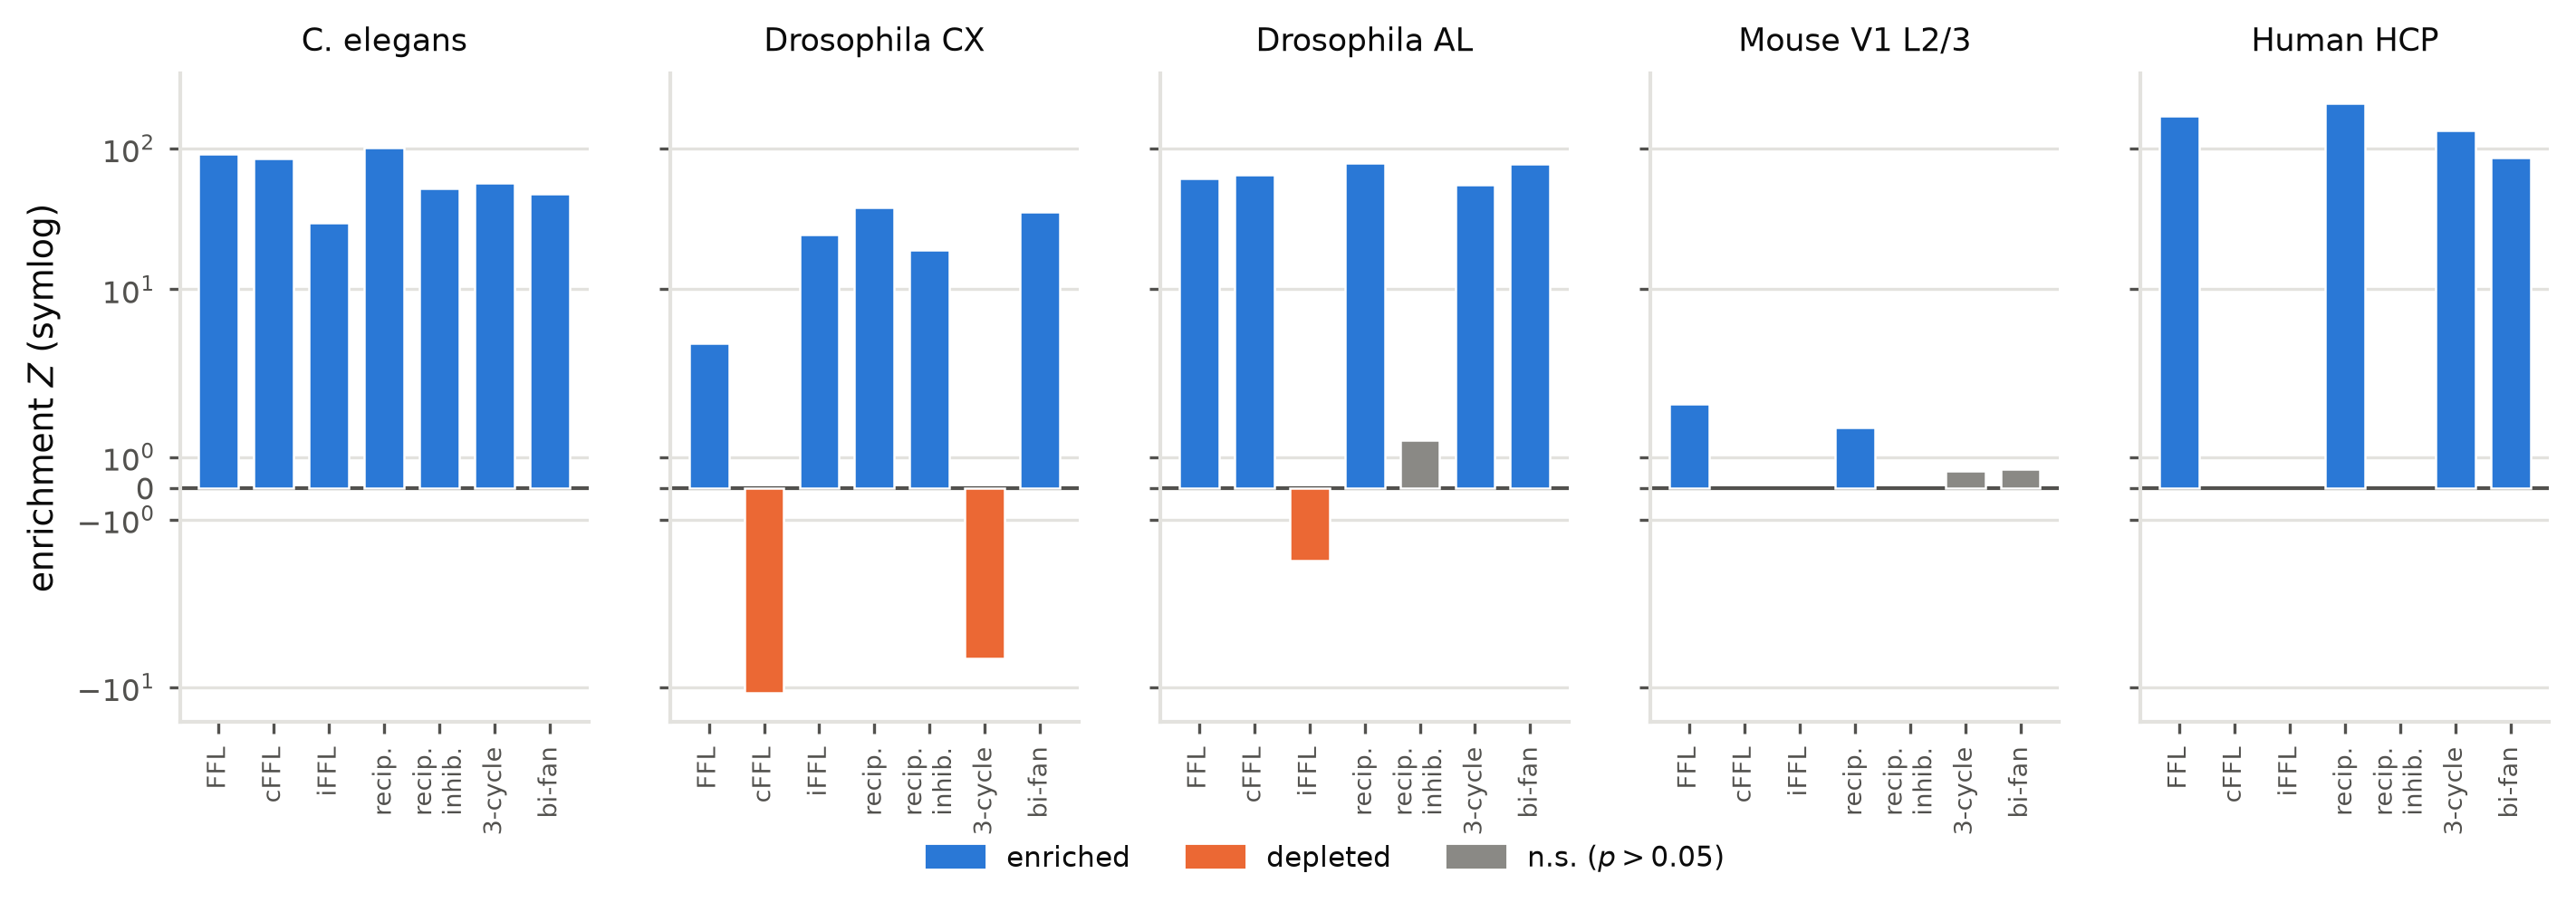
\includegraphics[width=0.95\textwidth]{figures/fig_motifs.png}
\caption{\textbf{Motif enrichment against a degree-preserving null}, $K = \NMotifNulls$
surrogates per network, exact counts, symlog axis. Colour encodes the outcome of each
test rather than the network, because the point is that the outcome differs between
networks: the \textit{Drosophila} central complex \emph{depletes} coherent feedforward
loops and directed 3-cycles, the antennal lobe depletes incoherent feedforward loops,
and mouse V1 L2/3 is close to its null throughout. Bars appear only where the dataset
supports the motif's definition --- coherent and incoherent feedforward loops require
synaptic valence, which diffusion tractography does not carry and which the mouse
release does not supply in connected form. The human column's magnitudes reflect an
almost entirely reciprocal tractography graph rather than a stronger biological effect
(see text).}
\label{fig:motifs}
\end{figure*}

Enrichment is real and often large, but it is not uniform, and the recomputation does
not support the description of these motifs as conserved across phylogeny. Of the
$\NMotifTests$ interpretable (network, motif) tests, $\NMotifEnriched$ are significantly
enriched, $\NMotifDepleted$ are significantly \emph{depleted}, and $\NMotifNull$ are
indistinguishable from the degree-preserving null.

Figure~\ref{fig:motifs} shows the pattern. In \textit{C. elegans} every motif is
strongly enriched: feedforward loops reach
$Z = \ZCeleFfl$ and reciprocal pairs $Z = \ZCeleRecip$. The \textit{Drosophila} central
complex breaks the pattern in the coordinate the motif literature cares about most ---
its coherent feedforward loops are depleted, $Z = \ZDrosCXCffl$, against an enrichment
of $\ZCeleCffl$ in the worm --- while its reciprocal pairs remain enriched
($Z = \ZDrosCXRecip$) and its directed 3-cycles are depleted ($Z = \ZDrosCXCyc$). Mouse
V1 L2/3 is the clearest case: no motif in that network is enriched by more than
$Z = \ZMouseFfl$, and directed 3-cycles ($Z = \ZMouseCyc$) and bi-fans are
indistinguishable from chance. Correspondingly, the normalised significance profiles of
the two sign-attributed fly circuits agree with each other no better than either agrees
with the worm ($\SPFlyFly$ for fly--fly, against $\SPWormFly$ and $\SPWormFlyAL$ for
worm--fly), so what is conserved is not a profile shape but the presence of some excess
somewhere.

Four qualifications belong with these numbers rather than in a footnote. First,
sign-attributed motifs are reported only for \textit{C. elegans} and \textit{Drosophila};
for the mouse and human networks the coherent and total feedforward loop counts would be
equal by construction (\S\ref{sec:data}), so quoting a coherent-FFL enrichment there
reports a topological result under a biological name. Second, the enrichment is measured
against a degree-preserving ensemble, and because Dale's principle is automatically
preserved by double-edge swaps, no part of this enrichment can be attributed to
excitatory/inhibitory organisation. Third, the very large $Z$-scores in the human row
($Z = \ZHumanFfl$ for feedforward loops) should not be read as a stronger biological
result than the invertebrate ones: HCP tractography is an essentially undirected
network, in which almost every edge is reciprocal, and a degree-preserving null of such
a graph is a poor match for it in ways that have nothing to do with computation. Fourth,
and most importantly for what follows: overrepresentation is a statement about a graph,
not about a computation. The remainder of the paper asks what, if anything, it buys.

\subsection{The motif-preserving ensemble}
\label{sec:res-null}

\begin{table*}[t]
\centering\small
\caption{\textbf{Validation of the motif-preserving ensemble.} The chain must hit its
target census, genuinely randomise, and not reproduce structure it was not asked to
preserve. Columns 2--3: worst-case relative error across the six targeted motif counts,
and the fraction of chains meeting the 2\% convergence criterion. Columns 4--5: edge
overlap with the empirical connectome for the motif-matched (L3) and degree-matched
(L2) ensembles --- L3 is close to the unconstrained level, so it is not the
connectome in disguise. Columns 6--7: mean pairwise overlap \emph{between} ensemble
members, as evidence of mixing. L3 members are somewhat less mutually distinct than L2
members, which is expected because the constrained set is a subset of the unconstrained
one; what matters is that they remain far from identical, so the chain explores the
constraint surface rather than collapsing onto one region of it. This is empirical
evidence of adequate mixing, not a proof of uniform sampling. Columns 8--10: bi-fan
counts, a 4-node motif deliberately excluded from the objective, reproduced neither in
value nor in a consistent direction, confirming the chain constrains 3-node structure
specifically rather than reconstructing the graph.}
\label{tab:nullval}
\resizebox{\textwidth}{!}{%
\begin{tabular}{lrrrrrrrrr}
\toprule
& \multicolumn{2}{c}{\textbf{Target match}} & \multicolumn{2}{c}{\textbf{Overlap w/ real (\%)}}
& \multicolumn{2}{c}{\textbf{Pairwise overlap (\%)}}
& \multicolumn{3}{c}{\textbf{Held-out bi-fan count}} \\
\cmidrule(lr){2-3}\cmidrule(lr){4-5}\cmidrule(lr){6-7}\cmidrule(lr){8-10}
\textbf{Network} & \textbf{max err (\%)} & \textbf{conv.\ (\%)} & \textbf{L3} & \textbf{L2}
& \textbf{L3} & \textbf{L2} & \textbf{empirical} & \textbf{L3} & \textbf{L2} \\
\midrule
\textit{C. elegans} & 0.3 & 100 & 13.9 & 11.6 & 21.0 & 11.1 & 118,612 & 179,732 & 65,882 \\
\textit{Drosophila} CX & 0.2 & 100 & 20.5 & 19.9 & 22.4 & 20.4 & 824,107 & 647,161 & 573,668 \\
\textit{Drosophila} AL & 0.1 & 100 & 43.9 & 40.0 & 45.6 & 38.9 & 12,622,936 & 12,038,186 & 9,058,482 \\
Mouse V1 L2/3 & 0.9 & 100 & 10.6 & 10.7 & 10.7 & 10.4 & 5,826 & 5,930 & 5,594 \\
Human HCP & 0.5 & 100 & 11.4 & 7.8 & 20.3 & 7.9 & 129,726 & 243,934 & 46,585 \\
\bottomrule
\end{tabular}}
\end{table*}


Table~\ref{tab:nullval} reports the three properties the annealed ensemble has to have
simultaneously. The chains reach the empirical census to within
$\AnnealErrCeleVal$ worst-case relative error on \textit{C. elegans} across all six
targeted motif counts, and converge on every network in the set, while retaining only
$\OverlapCele$ edge overlap with the empirical connectome --- against
$\OverlapLtwoCele$ for an unconstrained degree-preserving rewiring. The motif-matched surrogates are therefore not the
connectome in disguise: they agree with it on the motif census and are otherwise as
randomised as a standard null.

The held-out statistic confirms that the constraint is specific. Bi-fan counts, a
4-node motif deliberately excluded from the annealing objective, are not reproduced by
the L3 ensemble, and --- the point that matters --- they are not even displaced in a
consistent direction. In \textit{C. elegans} the empirical count is $\BifanRealCele$
against $\BifanLthreeCele$ for the motif-matched ensemble, an overshoot; in the
\textit{Drosophila} central complex it is $\BifanRealDrosCX$ against
$\BifanLthreeDrosCX$, an undershoot. Constraining the 3-node census therefore neither
fixes nor systematically biases 4-node structure. The chain constrains exactly the
structure whose contribution the ladder is designed to isolate and leaves higher-order
structure free, which is what distinguishes L3 from a partial reconstruction of the
connectome.

One further property is worth stating because the whole rung depends on it: the
constraint has to be \emph{binding}. If the empirical census were within ordinary
sampling range of the unconstrained ensemble, L3 would be a relabelled L2 and the
L2\,$\rightarrow$\,L3 contrast would be measuring nothing. It is not: the enrichment
$Z$-scores of \S\ref{sec:res-motifs} are the distance between exactly these two
ensembles' censuses, and they run from $Z = \ZMouseFfl$ in the least-enriched network to
$Z = \ZHumanRecip$ in the most. Except in mouse V1, where the census is close to its null
by construction and the contrast is correspondingly uninformative, L2 and L3 are
separated by tens to hundreds of null standard deviations in the coordinates the chain
constrains.

One asymmetry should be stated rather than left to the table. The L3 ensemble's members
are somewhat more similar to \emph{each other} than the unconstrained ensemble's members
are (mean pairwise edge overlap $\PairwiseLthreeCele$ against
$\PairwiseLtwoCele$ in \textit{C. elegans}), which is expected --- a constrained set is
smaller than the set that contains it --- but it means the L3 rung has less ensemble
diversity than L2 at equal instance count. We report the pairwise overlap for every
network so that this is visible, and we note that it works against detecting an L2--L3
difference only by inflating L3's variance, not by suppressing a mean difference.

\subsection{Protocol sensitivity}
\label{sec:res-protocol}

Before comparing rungs we fix what the benchmark can detect. Under an all-to-all
protocol, a reservoir with its recurrent matrix set to zero scores $\ZeroRecFull$ on
SHD while the \textit{C. elegans} connectome scores $\ZeroRecFullConn$: the recurrent
matrix is not used, and no structural comparison run in that regime can be informative.
Under the sensory/motor-disjoint protocol used throughout this paper, the same
zero-recurrence control falls to $\ZeroRecSplit$ against a chance level of
$\ChanceLevel$, while the connectome reaches $\ZeroRecSplitConn$. Task-relevant signal
must now traverse the recurrent graph, so differences between networks are attributable
to wiring.

\subsection{Decomposing performance across the ladder}
\label{sec:res-ladder}

\begin{table*}[t]
\centering\small
\caption{\textbf{SHD test accuracy (\%) by ladder rung}, mean $\pm$ 95\% CI over
15 surrogates per rung. Every rung is matched on node count, edge count, spectral
radius and input projection; adjacent rungs differ in exactly one structural
property. Chance is 5.0\%; a zero-recurrence network scores \ZeroRecSplit{} under
this protocol.}
\label{tab:ladder_acc}
\resizebox{\textwidth}{!}{%
\begin{tabular}{lrrrrr}
\toprule
\textbf{Rung} & \textit{C. elegans} & \textit{Drosophila} CX & \textit{Drosophila} AL & Mouse V1 L2/3 & Human HCP \\
\midrule
L0 density & 37.1\,$\pm$\,1.0 & 42.7\,$\pm$\,0.6 & 39.9\,$\pm$\,1.3 & 39.8\,$\pm$\,1.0 & 38.8\,$\pm$\,0.7 \\
L1 $+$degree & 36.8\,$\pm$\,1.1 & 38.0\,$\pm$\,1.3 & 31.9\,$\pm$\,1.9 & 32.1\,$\pm$\,1.9 & 39.1\,$\pm$\,1.2 \\
L2 $+$valence & 36.9\,$\pm$\,1.1 & 34.8\,$\pm$\,1.5 & 30.6\,$\pm$\,1.7 & 31.5\,$\pm$\,1.9 & 38.3\,$\pm$\,1.5 \\
L3 $+$motifs & 33.1\,$\pm$\,1.4 & 33.9\,$\pm$\,1.6 & 27.1\,$\pm$\,2.7 & 31.8\,$\pm$\,1.4 & 32.4\,$\pm$\,1.4 \\
L4 connectome & 36.3\,$\pm$\,1.7 & 26.3\,$\pm$\,2.0 & 28.2\,$\pm$\,1.6 & 31.8\,$\pm$\,1.8 & 38.6\,$\pm$\,1.0 \\
\bottomrule
\end{tabular}}
\end{table*}

\begin{table}[t]
\centering\small
\caption{\textbf{Contribution of each structural property}, as the difference between
adjacent ladder rungs in SHD accuracy (percentage points), with percentile-bootstrap
95\% CIs, Hedges' $g$, and Holm-corrected $p$-values across the whole family of
contrasts. $\ast$ marks $p_{\mathrm{Holm}} < 0.05$.}
\label{tab:contrasts}
\resizebox{\columnwidth}{!}{%
\begin{tabular}{llrlrr}
\toprule
\textbf{Network} & \textbf{Property added} & \textbf{$\Delta$ (pp)} &
\textbf{95\% CI} & \textbf{$g$} & \textbf{$p_{\mathrm{Holm}}$} \\
\midrule
\textit{C. elegans} & + degree sequence & -0.29 & [-1.78, +1.11] & -0.14 & 1.000 \\
\textit{C. elegans} & + valence placement & +0.15 & [-1.40, +1.70] & +0.07 & 1.000 \\
\textit{C. elegans} & + motif census & -3.80 & [-5.54, -2.04] & -1.46 & 0.005$\ast$ \\
\textit{C. elegans} & Empirical connectome & +3.16 & [+1.01, +5.24] & +0.99 & 0.115 \\
\textit{Drosophila} CX & + degree sequence & -4.65 & [-6.12, -3.36] & -2.31 & 0.000$\ast$ \\
\textit{Drosophila} CX & + valence placement & -3.16 & [-5.02, -1.29] & -1.14 & 0.045$\ast$ \\
\textit{Drosophila} CX & + motif census & -0.98 & [-3.13, +1.11] & -0.31 & 1.000 \\
\textit{Drosophila} CX & Empirical connectome & -7.60 & [-10.05, -5.07] & -2.04 & 0.000$\ast$ \\
\textit{Drosophila} AL & + degree sequence & -8.02 & [-10.35, -5.85] & -2.38 & 0.000$\ast$ \\
\textit{Drosophila} AL & + valence placement & -1.28 & [-3.72, +1.30] & -0.34 & 1.000 \\
\textit{Drosophila} AL & + motif census & -3.50 & [-6.70, -0.50] & -0.76 & 0.465 \\
\textit{Drosophila} AL & Empirical connectome & +1.06 & [-1.85, +4.23] & +0.24 & 1.000 \\
Mouse V1 L2/3 & + degree sequence & -7.65 & [-9.66, -5.65] & -2.51 & 0.000$\ast$ \\
Mouse V1 L2/3 & + valence placement & -0.63 & [-3.21, +1.96] & -0.16 & 1.000 \\
Mouse V1 L2/3 & + motif census & +0.30 & [-1.99, +2.59] & +0.09 & 1.000 \\
Mouse V1 L2/3 & Empirical connectome & +0.02 & [-2.21, +2.24] & +0.01 & 1.000 \\
Human HCP & + degree sequence & +0.34 & [-0.97, +1.69] & +0.18 & 1.000 \\
Human HCP & + valence placement & -0.82 & [-2.59, +1.02] & -0.31 & 1.000 \\
Human HCP & + motif census & -5.94 & [-7.96, -4.00] & -2.06 & 0.000$\ast$ \\
Human HCP & Empirical connectome & +6.25 & [+4.61, +7.90] & +2.52 & 0.000$\ast$ \\
\bottomrule
\end{tabular}}
\end{table}


\begin{figure*}[t]
\centering
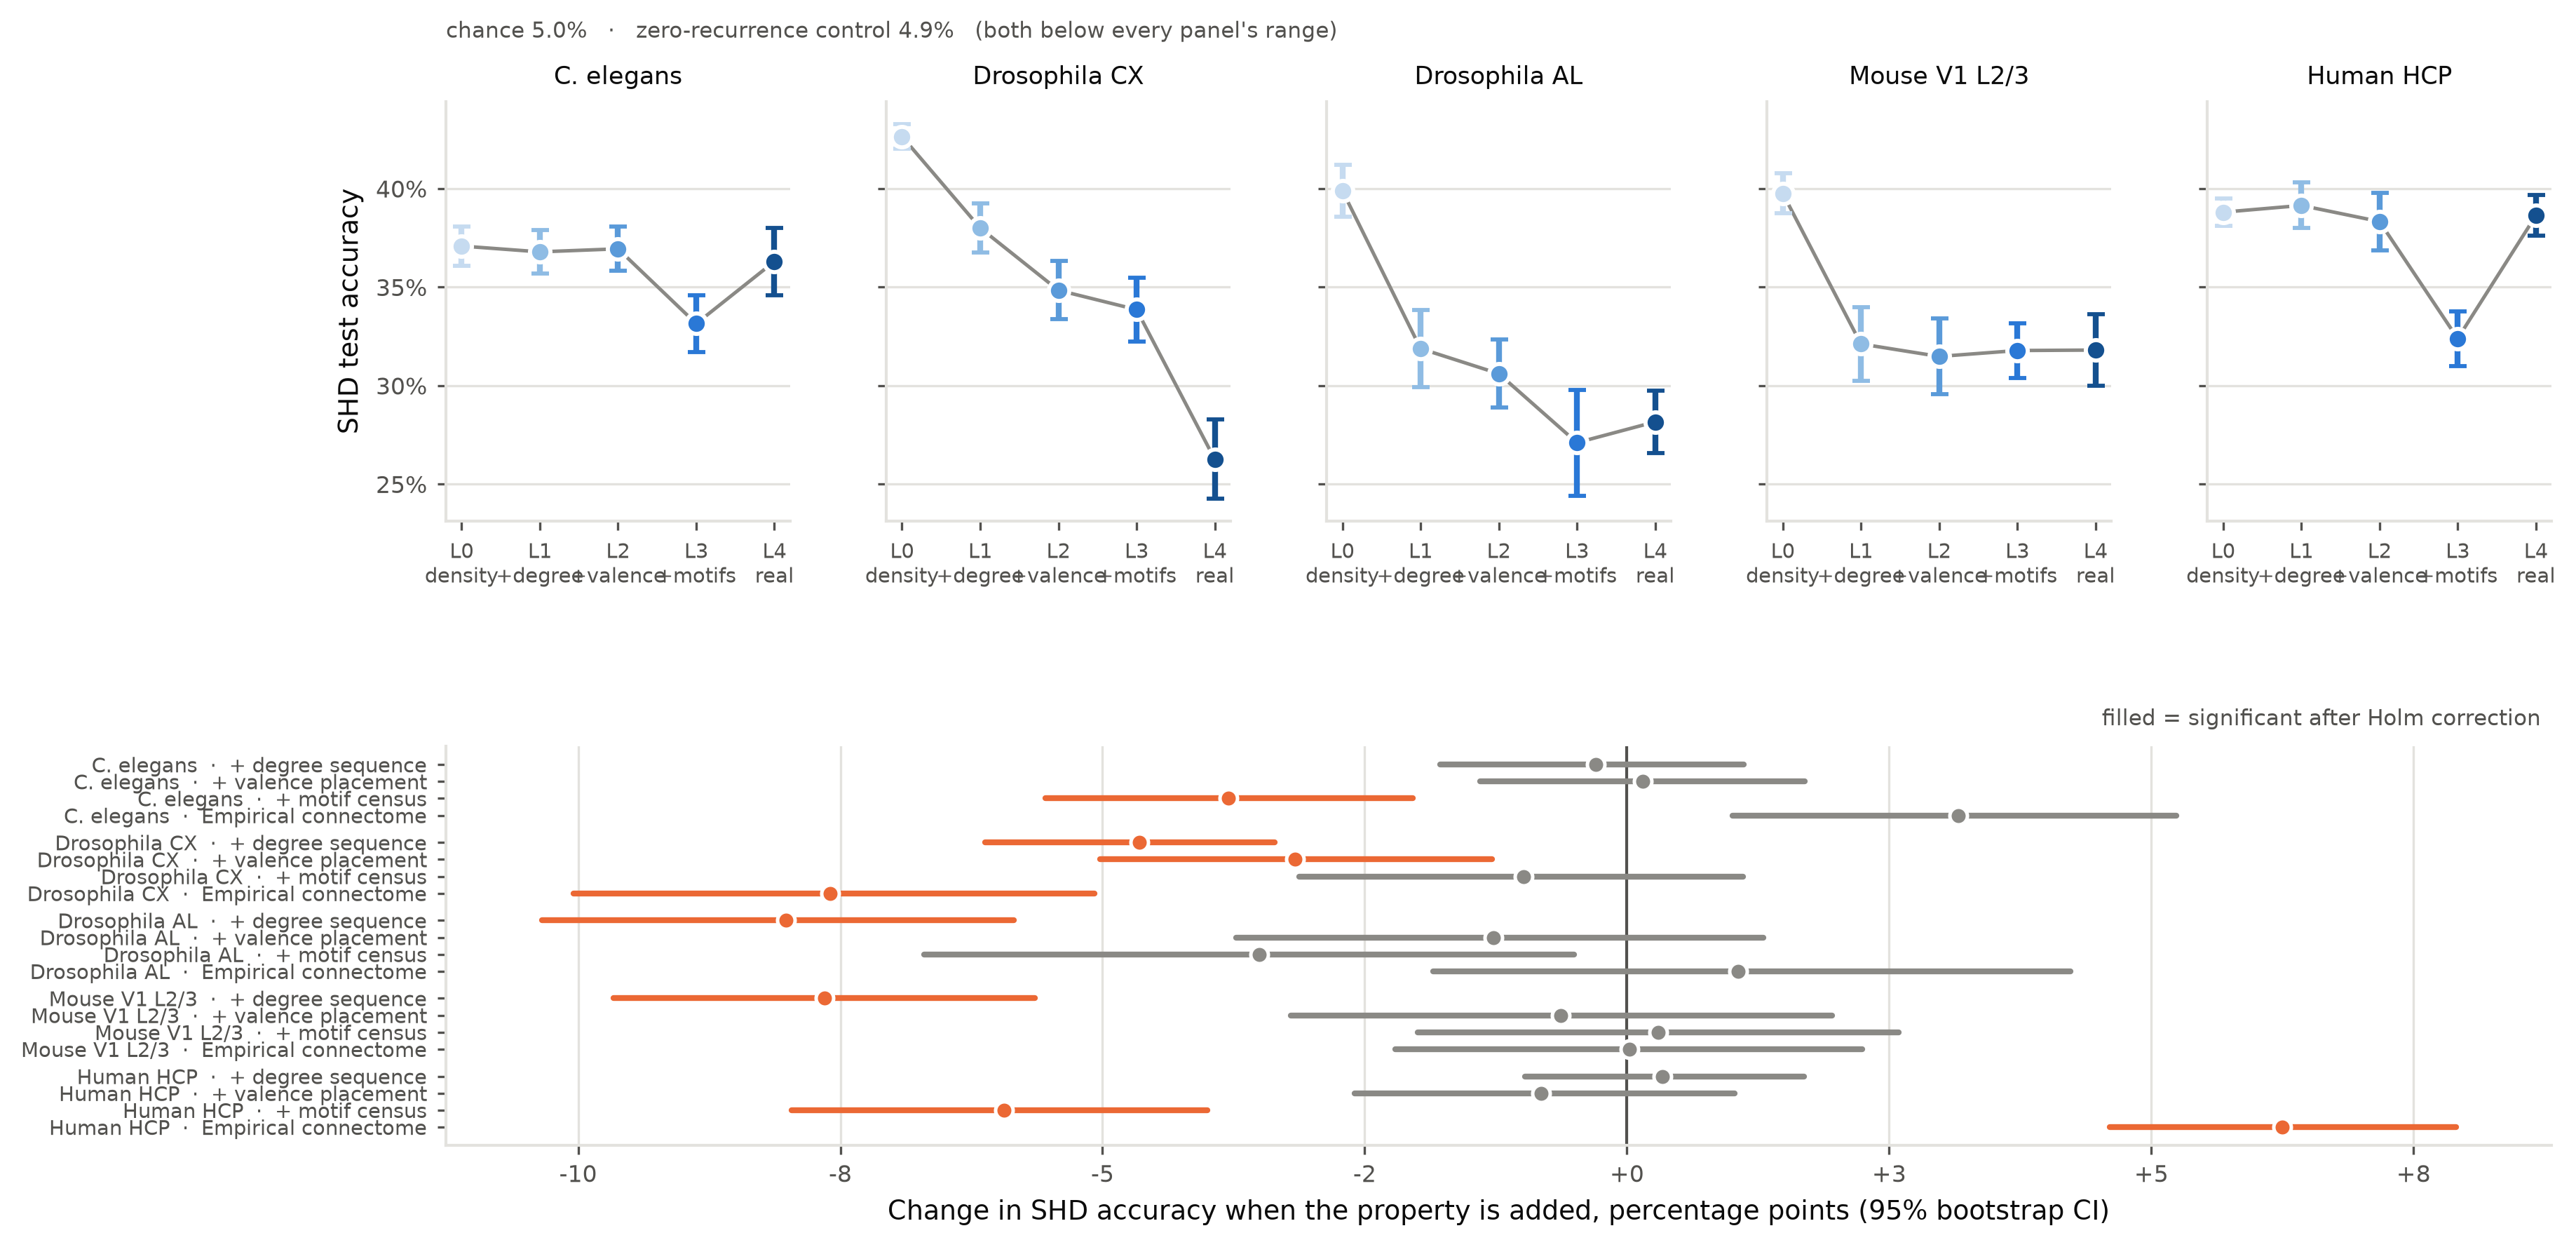
\includegraphics[width=0.95\textwidth]{figures/fig_ladder.png}
\caption{\textbf{Structural decomposition of reservoir performance on SHD.}
\textbf{Top:} mean accuracy with 95\% CIs at each ladder rung, per network. Each rung
adds one structural property to the rung on its left; all rungs are matched on node
count, edge count, spectral radius and input projection. Dotted line, chance; dashed
line, the zero-recurrence control. \textbf{Bottom:} the contribution of each property,
as the difference between adjacent rungs with bootstrap 95\% CIs; intervals spanning
zero indicate a property that does not measurably change performance.}
\label{fig:ladder}
\end{figure*}

Table~\ref{tab:ladder_acc} and Figure~\ref{fig:ladder} give the decomposition. We read it
property by property rather than as a count over the $\NLadderContrasts$ contrasts,
because the question is not how many differences reach significance but which structural
properties this benchmark is sensitive to and in which direction.

The direction is the first thing to say, because it is uniform and it is not the
direction the motif hypothesis predicts. \emph{Every} structural property that
measurably moves accuracy moves it \emph{down}. Each rung adds something the connectome
has and the rung below it does not, and at every step where the effect is resolvable the
addition makes the network a worse reservoir.

\textbf{Degree sequence} (L0\,$\rightarrow$\,L1) is the largest single contributor:
significant after Holm correction in $\NDegreeSig$ of $\NDegreeTotal$ networks, median
effect $\DegreeEffectMedian$, largest $\DegreeEffectMax$ (Hedges'
$g = \DegreeEffectMaxG$).

\textbf{The motif census} (L2\,$\rightarrow$\,L3) is the contrast this paper was built to
measure: it adds the connectome's exact 3-node motif spectrum while holding degree
sequence and valence placement fixed, using the ensemble validated in
\S\ref{sec:res-null}. It is significant in $\NMotifSig$ of $\NMotifTotal$ networks, with
median effect $\MotifEffectMedian$ and largest $\MotifEffectMax$
($g = \MotifEffectMaxG$). This is not a negligible effect and we do not report it as
one --- it is comparable in size to the degree-sequence contrast --- but its sign is
negative. Imposing a connectome's motif structure on a degree- and valence-matched
surrogate costs accuracy on this task.

\textbf{Valence placement} (L1\,$\rightarrow$\,L2) --- returning inhibitory labels to the
neurons that carry them rather than permuting them across the graph --- is significant in
$\NValenceSig$ of $\NValenceTotal$, median $\ValenceEffectMedian$.

\textbf{The residual wiring} (L3\,$\rightarrow$\,L4) adds everything else about the
empirical graph: weights aside, its exact synapse-by-synapse identity. Significant in
$\NResidualSig$ of $\NResidualTotal$, median $\ResidualEffectMedian$, and it is the one
property whose sign is not consistent --- it helps in some networks and hurts in others.

\paragraph{What the design could have detected.}
A small measured effect and an underpowered design look identical in a table, so we state
the bound. With $\NinstancesLadder$ surrogates per rung and $\NLadderContrasts$ contrasts
in the family, the design has $\PowerLevel$ power to resolve a standardised effect of
$d = \MDEUncorrected$ uncorrected and $d = \MDEHolm$ at the Holm worst case. The
significant contrasts reported above sit at or beyond that bound; the non-significant
ones do not exclude moderate effects, and we do not claim they do.

\paragraph{The reading.}
The motif hypothesis, as we stated it in \S\ref{sec:intro} and as our own earlier work
asserted it, is that connectome motif structure confers a computational advantage over
matched controls. On this benchmark, in the fixed-reservoir regime, at matched size,
density, spectral radius and input projection, it does not. The measured effect of adding
the empirical motif census has the opposite sign, and it is large enough to detect in two
of five networks.

We are careful about what this licenses, because the uniform negative sign across
properties is itself informative about the probe. A reservoir with a linear decoder
rewards distributed, high-dimensional state. Connectome structure --- heavy-tailed degrees,
excess feedforward loops and reciprocal pairs --- concentrates and correlates activity,
which spends the dimensions such a decoder needs. That is a property of this probe as
much as of these graphs, and a different task with a different readout could order them
differently. What it does establish is that an Erd\H{o}s--R\'enyi comparison cannot be
used to argue the motif hypothesis on this benchmark, because that comparison comes out
against it.

\subsection{The ladder at a matched operating point}
\label{sec:res-rate}

\begin{table*}[t]
\centering\small
\caption{\textbf{The ladder at a matched operating point.} Each network is calibrated
individually, by bisection on its own spectral radius, to a common mean firing rate of
0.07; 10 surrogates per rung.
\textbf{Top:} SHD test accuracy (\%), mean $\pm$ 95\% CI, over the surrogates that
reached the target. \textbf{Bottom:} the spectral radius each topology required, averaged
over all surrogates including those that did not. 27 of
250 surrogates never reached the target rate: the bisection
saturates at the top of its bracket and the network still fires below target.
$^{\ast}$ marks a cell where some surrogates were excluded on that ground and
$\dagger$ one where all were --- the \textit{Drosophila} central complex is 66\%
inhibitory, so raising its gain raises its inhibition and its attainable rate is capped.
Accuracy differences that survive in Table~\ref{tab:ladder_acc} but not here were
differences in activity level rather than in wiring.}
\label{tab:rate_matched}
\resizebox{\textwidth}{!}{%
\begin{tabular}{lrrrrr}
\toprule
\textbf{Rung} & \textit{C. elegans} & \textit{Drosophila} CX & \textit{Drosophila} AL & Mouse V1 L2/3 & Human HCP \\
\midrule
\multicolumn{6}{l}{\emph{Test accuracy (\%)}} \\
L0 density & 39.0\,$\pm$\,1.2 & 41.9\,$\pm$\,0.6 & 42.0\,$\pm$\,0.8 & 41.0\,$\pm$\,0.9 & 41.0\,$\pm$\,1.2 \\
L1 $+$degree & 37.1\,$\pm$\,1.6 & 37.9\,$\pm$\,1.3 & 32.7\,$\pm$\,2.8 & 32.8\,$\pm$\,1.9 & 38.2\,$\pm$\,0.8 \\
L2 $+$valence & 36.1\,$\pm$\,1.3 & 35.1\,$\pm$\,1.9$^{\ast}$ & 31.0\,$\pm$\,1.7 & 32.4\,$\pm$\,1.9 & 38.6\,$\pm$\,1.1 \\
L3 $+$motifs & 35.0\,$\pm$\,1.4$^{\ast}$ & 39.0\,$\pm$\,5.0$^{\ast}$ & 28.6\,$\pm$\,2.2 & 32.8\,$\pm$\,1.8 & 34.3\,$\pm$\,1.4$^{\ast}$ \\
L4 connectome & 35.9\,$\pm$\,1.9 & $\dagger$ & 28.1\,$\pm$\,1.9 & 32.0\,$\pm$\,2.3 & 38.9\,$\pm$\,0.8 \\
\midrule
\multicolumn{6}{l}{\emph{Calibrated spectral radius $\rho$}} \\
L0 density & 1.22 & 1.15 & 1.12 & 1.15 & 1.17 \\
L1 $+$degree & 1.28 & 1.62 & 1.26 & 1.25 & 1.28 \\
L2 $+$valence & 1.26 & 5.96 & 1.36 & 1.23 & 1.28 \\
L3 $+$motifs & 1.41 & 5.79 & 1.38 & 1.21 & 1.46 \\
L4 connectome & 1.30 & 6.00 & 1.35 & 1.25 & 1.31 \\
\bottomrule
\end{tabular}}
\end{table*}


\begin{figure*}[t]
\centering
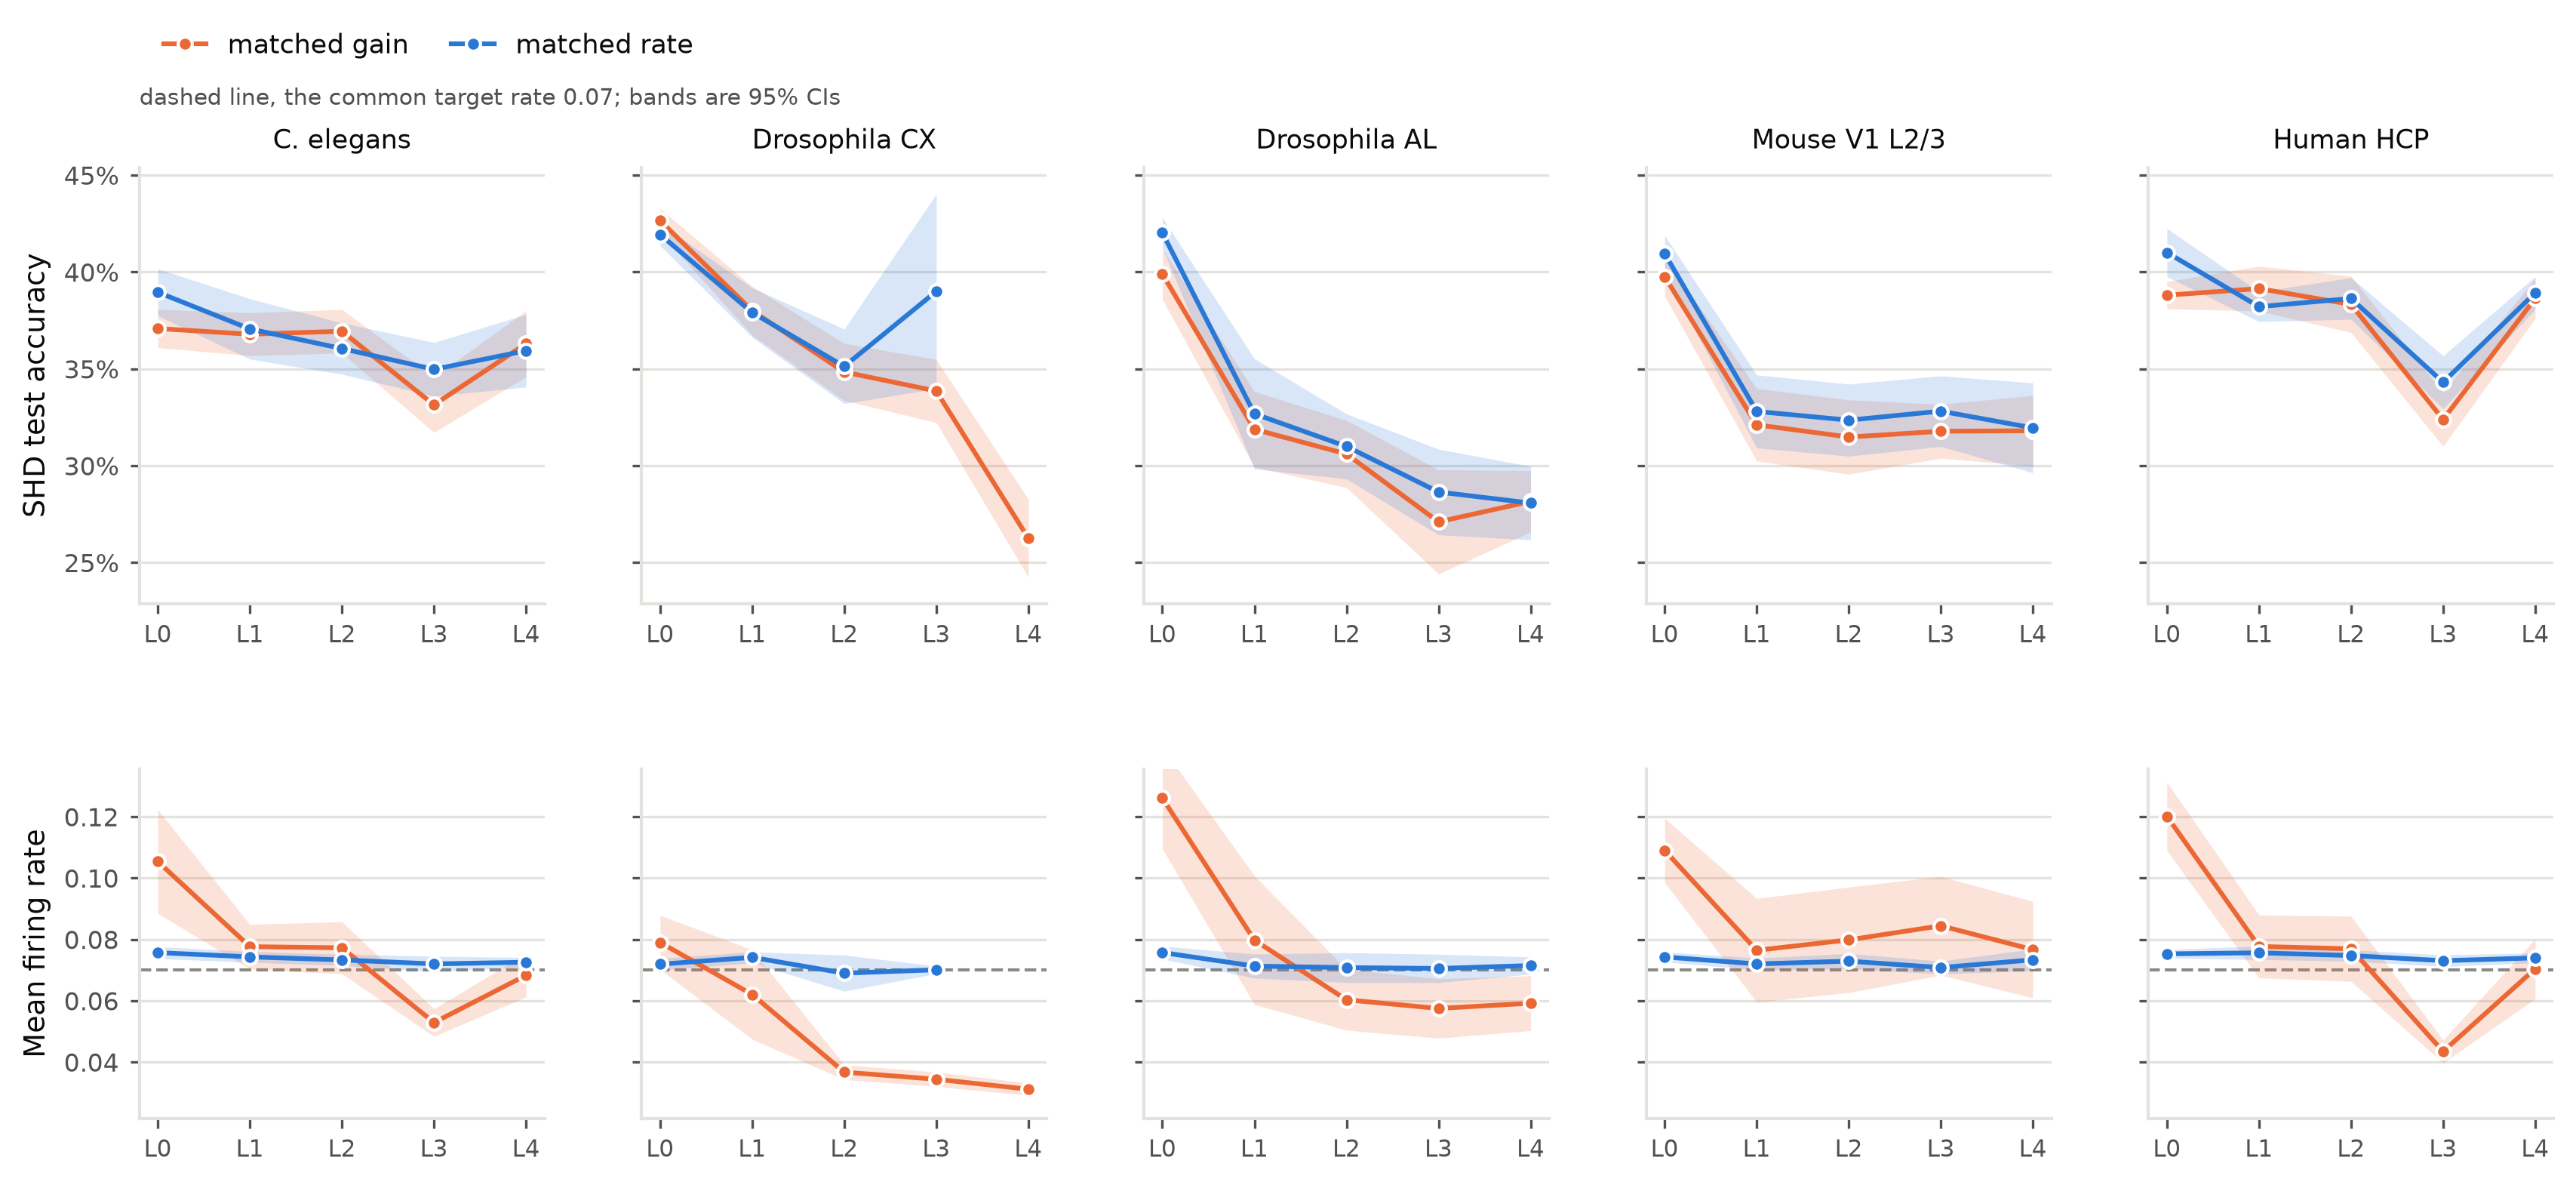
\includegraphics[width=0.95\textwidth]{figures/fig_rate_matched.png}
\caption{\textbf{The ladder at matched gain and at a matched operating point.} Colour
encodes the matching regime rather than the network, because the comparison is within a
network. Rungs are L0 density, L1 $+$degree, L2 $+$valence, L3 $+$motifs, L4 the
empirical connectome. \textbf{Top:} SHD test accuracy by rung under each regime.
\textbf{Bottom:}
mean firing rate. At a fixed spectral radius (orange) the rungs run at different rates,
and the accuracy ordering tracks the rate; calibrating each network individually to the
common rate (blue, dashed line) holds every network on the target. The accuracy decline
from L0 to L4 survives that correction. Cells whose calibration never reached the target
are omitted from the matched-rate series, which is why the \textit{Drosophila} CX panel
has no L4 point. Bands are 95\% CIs.}
\label{fig:rate_matched}
\end{figure*}

One asymmetry in Table~\ref{tab:ladder_acc} needs separating out before any of it can
be read as a statement about topology. The rungs are matched on spectral radius, but
they do not fire at the same rate: averaged over networks the Erd\H{o}s--R\'enyi rung
settles at $\RateLzero$ mean rate against $\RateLfour$ for the empirical connectome, a
factor of $\RateRatioLzeroLfour$. Across all runs firing rate is correlated with accuracy
($r = \RateAccCorr$), and it determines the synaptic-operation count outright. A
comparison at matched gain therefore confounds topology with operating point, in the
direction that flatters the unstructured control.

Recalibrating each network individually to a common mean rate of $\TargetRate$ removes
the confound, at the cost of letting spectral radius vary. Table~\ref{tab:rate_matched}
and Figure~\ref{fig:rate_matched} give the result, and it is not the one we expected.

\paragraph{Where the calibration fails, and why that is a result.}
Of $\NRateCells$ calibrated surrogates, $\NRateUnmatched$ never reach the target rate at
all: the bisection saturates at the top of its bracket and the network still fires below
target, in the worst case at $\RateUnmatchedWorst$ of it. $\NRateUnmatchedThere$ of the
$\NRateUnmatched$ are in one network, $\RateUnmatchedWhere$, whose edges are 66\%
inhibitory --- raising the gain in such a circuit raises its inhibition too, so its
attainable firing rate is bounded above by its own valence organisation. The effect
strengthens down the rungs, from none at L0 and L1 to every surrogate at L4, which
places the ceiling squarely on the empirical valence placement rather than on density. We exclude those cells from every matched-rate
statistic rather than averaging them in, since a cell that was not calibrated is not
rate-matched, and we report the exclusion because the ceiling is a property of the
network worth stating. That leaves $\NRateCompleteNetworks$ networks in which every rung
is fully matched, and the contrasts below are computed on those.

\paragraph{The operating point does not explain the gap.}
At a matched operating point the Erd\H{o}s--R\'enyi rung still outperforms the empirical
connectome, by $\RmLzeroMinusLfourMin$ to $\RmLzeroMinusLfour$ of accuracy in
percentage points, against
$\MgLzeroMinusLfourMin$ to $\MgLzeroMinusLfour$ for the same networks at matched gain.
The gap does not shrink; it is marginally larger. Firing rate is therefore a real
confound in the matched-gain comparison --- it is why we report both --- but it is not
what produces the unstructured control's advantage, and we were wrong to expect that it
would.

What the two versions together establish is narrower and firmer than either alone. On
this task, in this regime, connectome wiring is not merely no better than an
unstructured graph of the same size and density: it is measurably worse, and that
remains true when the networks are compared at the same activity level. Reading down the
rungs shows where the cost is incurred. The step that imposes the empirical degree
sequence, L0\,$\rightarrow$\,L1, accounts for $\RmDegreeShareMin$ to
$\RmDegreeShareMax$ of the whole decline; the three steps that follow --- adding valence
placement, the motif census and the remaining wiring --- divide the rest between them and
are individually small. Degree heterogeneity, not motif structure, is the
structural property this benchmark is sensitive to --- and its effect has the opposite
sign to the one the motif literature would predict for connectome structure as a whole.

We are explicit about what this does not show. It does not show that connectome wiring
is bad for computation, but that a degree-heterogeneous graph is a poor fixed reservoir
for a 20-class classification with a linear readout, which is one task in one regime and
not the objective any nervous system is under selection for. It does show that a
comparison against an Erd\H{o}s--R\'enyi control cannot be used to argue that connectome
structure confers a computational advantage, because on this benchmark that comparison
comes out the other way.

\subsection{Which rewiring counts as the null}
\label{sec:res-nullchoice}

This section and the three that follow it vary one argument of Eq.~\ref{eq:coupling} at a
time, holding the rest fixed, and report what that argument alone is worth. We begin with
$\mathcal{N}$, because it is the argument whose specification is least determinate and,
as it turns out, the one worth the most.

\begin{figure*}[t]
\centering
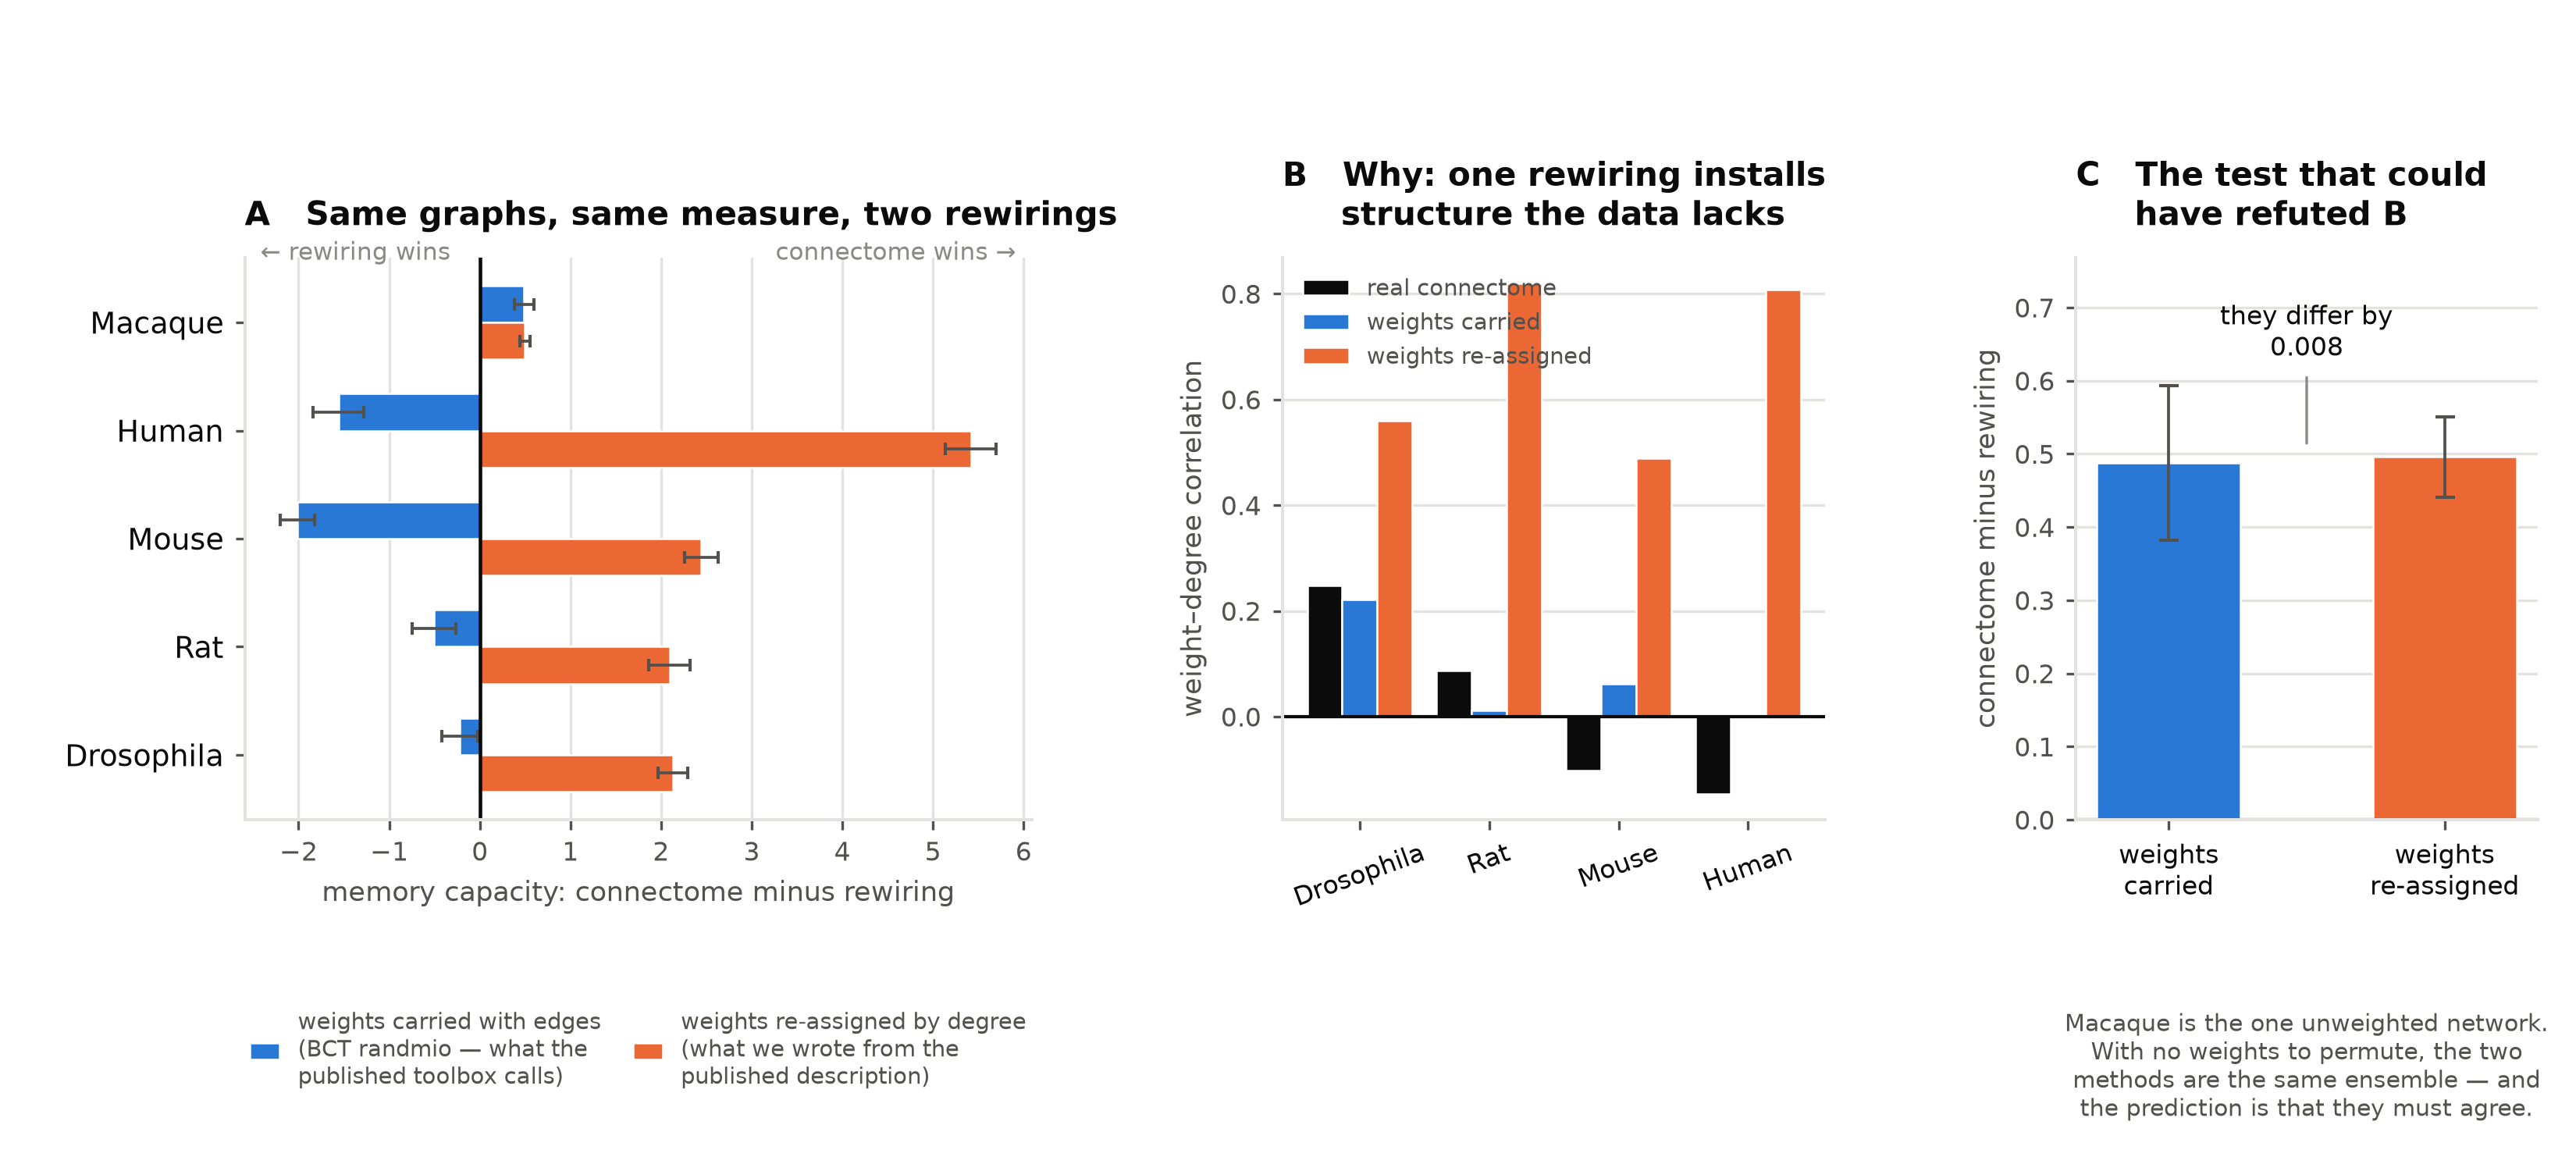
\includegraphics[width=0.98\textwidth]{figures/fig_null_choice.png}
\caption{\textbf{Two rewirings that answer to the same description, and the answers they
give.} \textbf{(A)} The empirical connectome's memory-capacity advantage over each of two
degree-preserving rewirings, at $\rho = 1$, with graded units. Same graphs, same inputs,
same delays, same readout, ten paired instances, 95\% confidence intervals. The only thing
that differs between a blue bar and the orange bar beside it is what happened to the edge
weights during randomisation: carried along with their edges, or re-assigned to the
rewired graph by endpoint-degree rank. Both procedures preserve the degree sequence and
the weight distribution exactly, and both are described in the literature as
``degree-preserving randomisation''. In four of five networks the pair points in opposite
directions. \textbf{(B)} The reason. Rank-reassignment does not only randomise: it
installs an association between an edge's weight and its endpoints' degrees that the
empirical graphs do not have (black) and that weight-carrying rewiring does not create
(blue). A reservoir whose largest weights sit on hub-to-hub edges is a poor one, so the
connectome's measured advantage over it is inflated. \textbf{(C)} The observation that
makes (B) an explanation rather than a story, because it could have come out the other
way. If the difference arises from permuting weights, then on a network with no weight
variation the two procedures are the same ensemble and must agree. Macaque is unweighted.
There the two measured advantages differ by $0.008$ capacity units, against a median
disagreement of $\NullDisagreeMedian$ across the rest of the set.}
\label{fig:nullchoice}
\end{figure*}

\begin{table*}[t]
\centering\small
\caption{\textbf{The connectome advantage depends on which rewiring it is compared
against, and on what a unit is.} Empirical connectome against two degree-preserving
rewiring ensembles at $\rho = 1$, the operating point of the published comparison, on the
five regional connectomes distributed with \texttt{conn2res}. \texttt{randmio} carries
each weight along with its edge; rank-reassignment rewires the topology and then
re-assigns the same multiset of weights by endpoint-degree rank. Both satisfy
``degree-preserving randomisation''. Identical graphs, inputs, delays and readout; ten
paired instances; paired $t$-test, $\ast$ marks $p < 0.05$. Absolute capacities are shown
because they establish whether a cell is informative: the human spiking row sits at the
floor and carries nothing, the other four do not.}
\label{tab:unitmodel}
\resizebox{\textwidth}{!}{%
\begin{tabular}{lrrrrr}
\toprule
& \textbf{Connectome} & \multicolumn{2}{c}{\textbf{BCT} \texttt{randmio}} & \multicolumn{2}{c}{\textbf{Rank-reassigned}} \\
\cmidrule(lr){3-6}
\textbf{Network} & \textbf{Capacity} & \textbf{Capacity} & \textbf{Difference} & \textbf{Capacity} & \textbf{Difference} \\
\midrule
\multicolumn{6}{l}{\emph{Graded-rate units} (\texttt{tanh})} \\
\quad Human & 11.46 & 13.02 & -1.56\,$\pm$\,0.28$^{\ast}$ & 6.04 & +5.42\,$\pm$\,0.28$^{\ast}$ \\
\quad Macaque & 8.67 & 8.19 & +0.49\,$\pm$\,0.11$^{\ast}$ & 8.18 & +0.50\,$\pm$\,0.06$^{\ast}$ \\
\quad Mouse & 7.19 & 9.20 & -2.01\,$\pm$\,0.19$^{\ast}$ & 4.75 & +2.44\,$\pm$\,0.19$^{\ast}$ \\
\quad Rat & 7.46 & 7.97 & -0.51\,$\pm$\,0.24$^{\ast}$ & 5.37 & +2.09\,$\pm$\,0.22$^{\ast}$ \\
\quad \textit{Drosophila} & 5.92 & 6.14 & -0.22\,$\pm$\,0.20 & 3.79 & +2.13\,$\pm$\,0.16$^{\ast}$ \\
\multicolumn{6}{l}{\emph{Spiking units} (LIF)} \\
\quad Human & 0.05 & 1.36 & -1.31\,$\pm$\,1.29 & 0.02 & +0.03\,$\pm$\,0.05 \\
\quad Macaque & 1.93 & 1.88 & +0.04\,$\pm$\,0.07 & 1.94 & -0.01\,$\pm$\,0.04 \\
\quad Mouse & 1.34 & 1.61 & -0.27\,$\pm$\,0.08$^{\ast}$ & 1.56 & -0.23\,$\pm$\,0.11$^{\ast}$ \\
\quad Rat & 1.22 & 1.20 & +0.02\,$\pm$\,0.05 & 1.16 & +0.06\,$\pm$\,0.07 \\
\quad \textit{Drosophila} & 1.09 & 1.09 & +0.00\,$\pm$\,0.01 & 0.97 & +0.12\,$\pm$\,0.25 \\
\bottomrule
\end{tabular}}
\end{table*}


Every comparison in this literature is a comparison against a rewiring, and the rewiring
is almost always specified in a phrase: \emph{degree-preserving randomisation}, or
\emph{randomised while preserving density and degree sequence}. That phrase does not
determine an ensemble. At least two constructions satisfy it, and they differ in what
happens to the weights:

\begin{itemize}[leftmargin=1.2em,itemsep=2pt,topsep=3pt]
\item \textbf{Weight-carrying rewiring.} Double-edge swaps move edges, and each weight
travels with the edge that carries it. The Brain Connectivity Toolbox routine
\texttt{randmio\_und\_connected} / \texttt{randmio\_dir\_connected}
\cite{rubinov2010complex,maslov2002specificity} does this, additionally rejecting swaps
that disconnect the graph. This is what \texttt{conn2res} calls, and therefore what the
published result was measured against.
\item \textbf{Rank-reassigned rewiring.} The binary topology is randomised by the same
swaps, and the original multiset of weight values is then re-assigned to the new edges in
order of endpoint-degree product. This preserves the degree sequence and the weight
\emph{distribution} exactly, and destroys the association between a weight and the edge
carrying it.
\end{itemize}

Both are defensible nulls and both answer to the published phrase. We wrote the second
one, believing we had written the first, and the error is instructive enough that we ran
both rather than deleting it: it preserves every marginal the description names, it
produced a clean and highly significant result, and nothing about its output indicated
that it was answering a different question. It was caught by reading the toolbox source,
not by anything in the numbers.

\paragraph{The two ensembles do not agree.}
Figure~\ref{fig:nullchoice}A shows the result and Table~\ref{tab:unitmodel} the full
design against both. Of $\NNullCells$ (network,
unit model) cells, the two nulls give the connectome's advantage \emph{opposite signs} in
$\NNullSignFlip$, and opposite \emph{significant} verdicts --- one says the connectome
leads, the other says it trails, both at $p < 0.05$ --- in $\NNullVerdictFlip$. The median
absolute disagreement between the advantage measured against one null and against the
other is $\NullDisagreeMedian$ capacity units, and the largest is $\NullDisagreeMax$. For
scale, these are differences of the same order as the effects the literature reports.

\paragraph{Which one reproduces the published direction.}
Against the weight-carrying ensemble --- the one the original toolbox builds --- the
graded-rate reservoir puts the connectome ahead in $\NBctRateLeads$ of
$\NBctRateNetworks$ networks and behind in $\NBctRateTrails$, median
$\BctRateMedian$. Against the rank-reassigned ensemble the same graphs, the same unit
model and the same operating point put it ahead in $\NRankRateLeads$ of
$\NRankRateNetworks$, median $\RankRateMedian$. The direction of the headline result in
this design is set by a choice that the method sentence does not record.

\paragraph{Why they differ, and a prediction that could have refuted it.}
The disagreement is not noise, and it has a structural cause specific enough to be
checked in advance (Fig.~\ref{fig:nullchoice}B,C). Sorting the weight multiset onto rewired edges by endpoint-degree
product does not merely randomise: it \emph{installs} an association between an edge's
weight and its endpoints' degrees. Across the $\NNullWeighted$ weighted networks,
carrying weights with their edges shifts the weight--degree correlation by a median of
$\NullShiftBct$ relative to the empirical graph, and never by more than
$\NullShiftBctMax$; rank-reassignment shifts it by $\NullShiftRank$. In mouse the
empirical association is slightly \emph{negative} ($\WDegMouseEmp$), \texttt{randmio}
returns $\WDegMouseBct$, and rank-reassignment returns $\WDegMouseRank$; in rat the
corresponding figures are $\WDegRatEmp$, $\WDegRatBct$ and $\WDegRatRank$. A null that
adds a property the data lacks is not a control for the absence of that property, and a
reservoir whose largest weights are concentrated on hub-to-hub edges is a poor one --- so
the connectome's advantage over it is inflated, in the direction and roughly the
magnitude we observed.

This account makes a prediction that would have falsified it cheaply: if the difference
comes from permuting weights, then on a network with no weight variation the two
constructions are the same ensemble and must agree exactly. One network in the set is
binary. On macaque the two nulls shift the weight--degree association by
$\WDegMacaqueBct$ and $\WDegMacaqueRank$ respectively --- that is, by nothing --- and
the connectome's measured advantage against them differs by $0.008$ capacity units,
against a median disagreement of $\NullDisagreeMedian$ elsewhere. It is the one cell in
Table~\ref{tab:unitmodel} where the choice of null provably cannot matter, and it is the
one cell where it does not.

\paragraph{What this does and does not establish.}
It does not show that either null is wrong. Rank-reassignment is a coherent ensemble and
a comparison against it is a coherent question --- it asks whether the \emph{placement} of
a connectome's weights matters given its degree sequence, which is a narrower and in some
ways sharper question than the one weight-carrying rewiring asks. What it shows is that
the two questions have different answers, that the phrase in general use does not
distinguish them, and that a reader cannot recover which was asked from the reported
number. A replication that constructs its own null from the published description is
therefore not a replication, and we include ours as an instance of that failure rather
than a warning about it.

\subsection{What a firing threshold does to the comparison}
\label{sec:res-unit}

The disagreement of \S\ref{sec:res-operating} has a candidate explanation that does not
involve the operating point at all, and it is checkable in one experiment.
\cite{suarez2024connectome} evaluate an echo state network of $\tanh$ units. We evaluate
a spiking leaky integrate-and-fire network. Those are not two implementations of one
model. A $\tanh$ unit responds to any input however small and is never silent; a LIF unit
below threshold emits nothing and contributes no variance to the readout at all.

We therefore ran both unit models over identical graphs, identical rewirings, identical
inputs, identical delays and an identical readout, on the five regional connectomes
distributed with \texttt{conn2res} --- the networks the published claim is made on, so
that the comparison inherits neither our subgraph extraction nor our binarisation.
$\NUnitEvaluations$ evaluations: $\NUnitNetworks$ networks $\times$ $\NUnitInstances$
paired instances $\times$ $\NUnitGains$ gains $\times$ two unit models.

All numbers in this subsection are measured against \texttt{randmio}, the ensemble the
published toolbox builds, for the reasons given in \S\ref{sec:res-nullchoice}.

\paragraph{With graded units, against the published null, we do not recover the published
direction.}
The empirical connectome leads its rewiring in $\NBctRateLeads$ of $\NBctRateNetworks$
networks at $\rho = 1$ and \emph{trails} significantly in $\NBctRateTrails$, median
$\BctRateMedian$ capacity units. Against the rank-reassigned ensemble, on the same graphs
at the same operating point in the same unit model, it leads in $\NRankRateLeads$ of
$\NRankRateNetworks$, median $\RankRateMedian$.

We do not read this as a refutation of \cite{suarez2024connectome}. Our harness differs
from theirs in the input projection, the delay set and the ridge solver as well as the
null, and any of those could account for a reproduction failure. What it does establish
is narrower and, we think, more useful: the choice of null \emph{alone} moves the result
by more than the effect being reported, which makes it a sufficient explanation for a
disagreement of this size without anything else having to be wrong. A reproduction
attempt that differs from the original in its null is not evidence against the original.

\paragraph{With spiking units the comparison is weaker still.}
On the same graphs the connectome leads significantly in $\NUnitSpkLeads$ of
$\NUnitSpkNetworks$ networks at $\rho = 1$ and trails significantly in
$\NUnitSpkTrails$; the median difference is $\UnitSpkMedianDiff$. Across the gain axis it
leads in $\UnitSpkFracLeadsAllGains$ of cells. Capacity itself falls by a factor of
$\UnitCapRatio$, from $\UnitCapRate$ to $\UnitCapSpiking$, so part of the weakening is
simply that there is less signal to resolve --- and the next paragraph asks whether the
rest is a fact about spiking units or about our choice of constants.

\paragraph{Is the spiking model simply untuned?}
The obvious objection is that we ran the spiking reservoir at one threshold, one leak and
one input scale, none of them tuned, and that a quiet network is a misconfigured one
rather than an informative one. That objection deserves an experiment rather than a
paragraph, and it gets one designed to refute us: we swept input gain from $\TuneGainLo$
to $\TuneGainHi$, threshold from $\TuneThreshLo$ to $\TuneThreshHi$ and two leaks ---
$\NTuneConfigs$ configurations, $\NTuneEvaluations$ evaluations --- and asked whether the
connectome advantage appears \emph{anywhere} the network is computing.

It does, in a few places, and not enough of them to sustain the strong claim. Of
$\NTuneCells$ (network, configuration) cells, $\NTuneHealthy$ are healthy by the
pre-stated criterion that the rewired control retains capacity above $0.5$ with fewer
than 80\% of units silent. Among those, the connectome leads significantly in
$\NTuneLeads$ and \emph{trails} significantly in $\NTuneTrails$, with a median difference
of $\TuneMedianDiff$. The configuration used in Table~\ref{tab:unitmodel} is not a
pathological corner: it sits within 20\% of the best capacity the sweep found.

So the accurate statement is not that the advantage is absent under spiking units but
that it is \emph{sporadic and inconsistent in sign} --- present in $\NTuneLeads$ of
$\NTuneHealthy$ well-conditioned settings, reversed in more of them, and negative at the
median. That is a weaker claim than the one we set out to make, and it is weaker in the
same direction as everything else in this section: once the null is the published one,
the unit model is no longer carrying a clean reversal, because there is no longer a clean
effect in either model for it to reverse.

\paragraph{The silencing mechanism, which we had previously reported as refuted.}
We predicted the mechanism before running it: a heavy-tailed degree sequence should leave
a connectome's low-degree neurons below threshold, silencing them, while no $\tanh$ unit
can be silent. The silencing is real and large --- $\UnitDeadSpiking$ of spiking units
never fire, against $\UnitDeadRate$ of rate units. Whether it is also \emph{differential}
is a question the choice of null decides, and we have had both answers. Against the
rank-reassigned ensemble the silencing gap did not predict the capacity gap and we
reported the prediction as failed. Against \texttt{randmio} it does: across
$\UnitSilenceGapN$ (network, gain) cells, the amount by which a connectome silences more
than its rewiring predicts the amount by which it loses capacity,
$r = \UnitSilenceGapR$, $p = \UnitSilenceGapP$.

We report the sign change rather than only the surviving result, because the two
conclusions were drawn from the same code and the same graphs and differ only in the
control. The supported version is the one measured against the published ensemble, and it
is a modest claim: differential silencing accounts for part of the spiking arm's
behaviour, in the predicted direction, leaving most of the variance unexplained.
Thresholding also compresses the measurement for every topology alike --- mean capacity
falls from $\UnitCapRate$ to $\UnitCapSpiking$, a factor of $\UnitCapRatio$ --- and that
compression is not differential at all.

\paragraph{A floor, declared.}
For the human network the spiking capacities are $0.049$ against $0.019$ --- both
effectively zero, so that network is uninformative in the spiking arm whatever it shows.
The remaining four retain capacities between $1.0$ and $1.9$ and do carry information.
The claim rests on those four.

\paragraph{What this licenses.}
Less than we hoped, and something worth saying anyway. We cannot claim a clean reversal
between unit models, because against the published null there is no clean effect in the
graded model to reverse. What we can claim is that the two model classes do not give the
same answer on identical graphs, that capacity in the spiking model is compressed by a
factor of $\UnitCapRatio$ so that effects of the reported size are near the resolution of
the measurement there, and that part of the difference tracks differential silencing. The
practical consequence is unchanged by the weakening: the connectome-reservoir result is
routinely invoked as motivation for neuromorphic architectures, neuromorphic hardware is
spiking, and the evidence that the property survives the transfer does not exist in
either direction yet.

\subsection{The contrast changes sign along the gain axis}
\label{sec:res-operating}

\begin{figure*}[t]
\centering
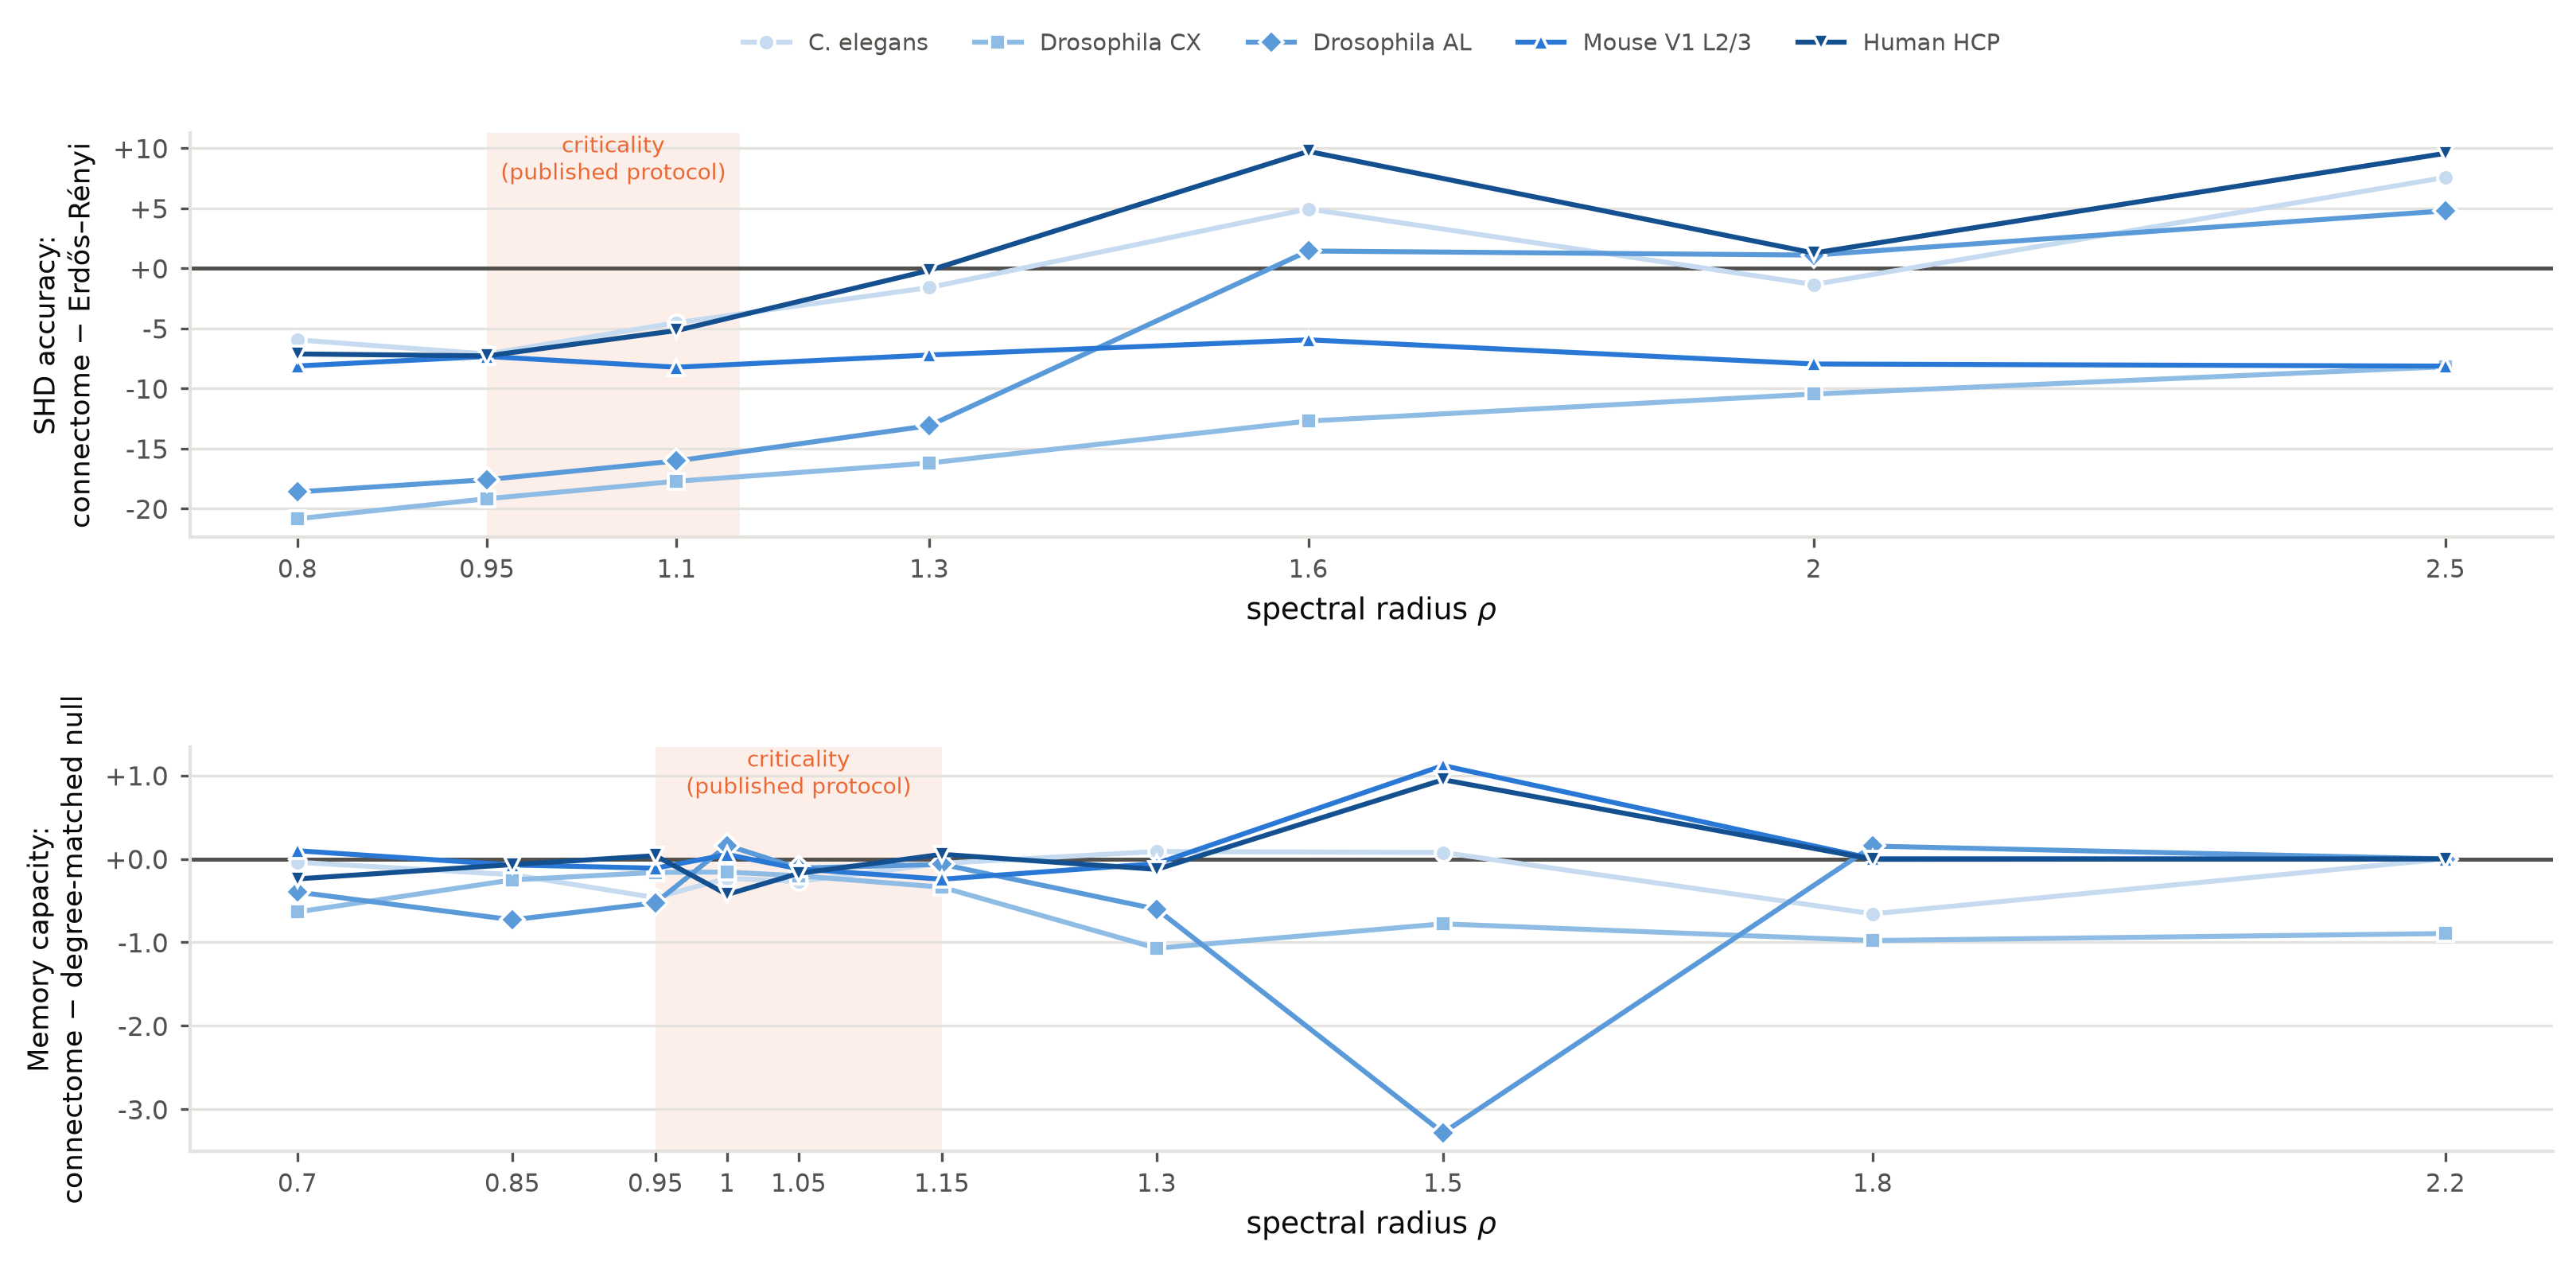
\includegraphics[width=0.95\textwidth]{figures/fig_operating_point.png}
\caption{\textbf{Where the comparison is made decides what it finds.} Both panels plot a
\emph{contrast}, not a performance curve, so that zero is the line that matters: below it
the connectome leads, above it the null does. \textbf{Top:} SHD accuracy, empirical
connectome minus the Erd\H{o}s--R\'enyi rung. \textbf{Bottom:} linear memory capacity,
empirical connectome minus the degree-preserving null --- the quantity and the control
used by \cite{suarez2024connectome}. The shaded band marks the critical region
($\rho \approx 1$) at which that comparison is reported. A published result of this kind
is a single point on one of these curves.}
\label{fig:operating}
\end{figure*}

Everything reported so far was measured at one operating point. \S\ref{sec:res-rate}
showed that the choice of operating point is not innocuous even when spectral radius is
held fixed. The question this raises is sharper than a robustness check, because the
literature reaches the opposite conclusion to ours on closely related measurements, and
does so at a different point on the same axis.

Su\'arez et al.~\cite{suarez2024connectome} report that empirical connectomes have significantly greater
linear memory capacity than degree-preserving rewirings, and report it \emph{at
criticality}, at a spectral radius of $1$. Our ladder is evaluated at
$\rho = \SpectralRadius$ and finds the opposite, on that same probe
(\S\ref{sec:res-dynamics}). Both measurements can be right, and we show that they are: the
contrast is not a fixed property of the pair of graphs being compared. It changes sign
along the gain axis.

\paragraph{Sweeping the axis.}
We re-ran the full ladder across $\NGainPoints$ spectral radii from $\GainGridLo$ to
$\GainGridHi$, $\NinstancesGain$ surrogates per rung per gain, each surrogate swept across
the whole axis so that curvature in $\rho$ is not confounded with surrogate-to-surrogate
variation. Of $\NGainCells$ evaluations $\NGainCellsFailed$ failed and are excluded and
counted rather than averaged in.

Two things follow, and the first is not what we expected to find.

\emph{On task accuracy the published direction does not appear, at any operating point we
tested including criticality.} At $\rho = \RhoCritical$ the Erd\H{o}s--R\'enyi rung leads
the empirical connectome in $\NGainNullLeadsAtCritical$ of $\NGainNetworks$ networks, with
every one of those differences significant against its own paired instance variation;
the median gap is $\GapAtCritical$. At $\rho = \RhoOurs$ it is $\GapAtOurs$. Whatever
advantage connectome topology has at criticality, it is not visible in the accuracy of a
linear readout on this task.

This is consistent with what has recently been reported from a hyperparameter sweep of
the \textit{C.\ elegans} connectome against Erd\H{o}s--R\'enyi, Watts--Strogatz and
shuffled controls \cite{hyperparam2026determinants}, which finds the connectome in a
lower-peak-performance, lower-sensitivity regime and notes that the
connectome-versus-null contrast varies with raw spectral radius. Our contribution on this
point is not the variation, which that work identifies, but its extent.

\emph{The contrast is not merely gain-dependent; it is not a constant of the pair being
compared.} It changes sign
along the axis in $\NGainSignFlip$ of $\NGainNetworks$ networks, with the contrast
significant on both sides of the crossing in each case, and the largest within-network
swing is $\GapSwingMax$ of accuracy --- several times the size of any structural effect in
\S\ref{sec:res-ladder}. In those networks the connectome catches the unstructured rung and
overtakes it above $\rho \approx 1.3$. In the remaining two the unstructured rung leads
significantly at every gain on the grid. We note the disagreement plainly:
\cite{hyperparam2026determinants} reports the connectome-versus-null relationship as
consistent across the regimes it tests, and we find a reversal. The two are not
straightforwardly comparable --- that work sweeps one connectome on task-agnostic probes,
ours sweeps five on task accuracy, and our own probe-based sweep is underpowered
(below) --- so we record this as a discrepancy to be resolved rather than as a
correction. The direction of the comparison is therefore a
joint property of the topology \emph{and} the regime, and a single number reported for it
is a number about both.

\paragraph{Attempting the published comparison directly, and failing to resolve it.}
The bottom panel of Figure~\ref{fig:operating} repeats the measurement the published claim
rests on: linear memory capacity, empirical connectome against a degree-preserving null,
across $\NMemGainPoints$ gains from $\MemGridLo$ to $\MemGridHi$, ten surrogates per rung
per gain, paired by instance.

We do not detect the reported advantage. At $\rho = \MemRhoCritical$ --- the published
operating point --- the connectome leads in $\NMemAdvPosAtCritical$ of $\NMemNetworks$
networks by the sign of the mean, and in $\NMemAdvSigAtCritical$ of $\NMemNetworks$ once
the paired confidence interval is taken into account. The median difference is
$\MemAdvAtCritical$ capacity units, against the null.

\emph{This is a non-detection and not a refutation, and the distinction is the whole of
it.} Our design at this operating point resolves a median effect of $\MemMDEMedian$
capacity units at $\PowerLevel$ power --- $\MemMDEFracMedian$ of the null network's own
capacity. An advantage of the size that would be scientifically interesting here is
comfortably inside our confidence intervals. On $\NMemPowered$ of $\NMemNetworks$
networks the variance is low enough to resolve $\MemMDEFracMin$ of capacity, and there
the difference is $+0.05 \pm 0.11$; on the other four the attempt is uninformative, and we
say so rather than reporting four null results as though they were evidence.

Several differences from the original could account for a real effect going undetected
here, and we have not isolated which. Our networks are size-matched induced subgraphs of
$\NnodesTarget$ nodes rather than whole released connectomes; our spiking reservoir is a
binary-weight LIF network rather than a rate model; and our memory-capacity estimator,
input scaling and washout are our own. We report the attempt because a reader deciding
what to believe about the published result should know that an independent implementation
did not see it, and should equally know that this implementation could not have seen it
unless it were very large.

\paragraph{Against an unstructured graph the direction is consistent.}
One asymmetry survives the power problem, because it is large. The published comparison
is against a \emph{degree-preserving} null. Against the Erd\H{o}s--R\'enyi rung the
connectome's memory capacity is lower at essentially every gain and in every network, by
margins that reach several capacity units --- far outside the intervals above. Whatever
the degree sequence and the wiring buy relative to each other, they do not recover what
is lost relative to an unstructured graph of the same size and density. This is the same
ordering the accuracy sweep gives, and the same one the ladder gives at a fixed gain.

\paragraph{Where the sweep stops being a comparison.}
A gain axis has an end, and past it the question dissolves. As $\rho$ grows the reservoir
saturates: every neuron fires at every step, the readout features stop varying, and the
state carries no information about the input regardless of how it is wired. We record the
effective rank of the readout features for every cell as a fraction of their number, so
that regime is identifiable by a number rather than inferred from a surprising accuracy.
It falls from $\FeatureRankAtOurs$ at $\rho = \RhoOurs$ to $\FeatureRankAtMaxGain$ at the
top of the grid. Of $\NGainCells$ evaluations, $\NGainCellsFailed$ failed outright and are
excluded and counted rather than averaged in as missing values.

We therefore do not rest the sign change on the saturated end of the axis. The crossing
reported above occurs between the critical region and $\rho = \RhoOurs$, where the state
is still high-rank in every network, and the far end of the sweep is shown for
completeness rather than used as evidence.

\paragraph{Two protocols, two questions.}
Neither way of choosing an operating point is wrong, and the difference between them is
not a matter of care. Comparing each network at its own optimum asks how good a topology
can be made to look when the rest of the model is tuned for it; comparing at a common
point asks what the topology does to a network held otherwise fixed. Under the first
protocol the rungs peak at different gains --- median $\BestRhoLzero$ for the
Erd\H{o}s--R\'enyi rung against $\BestRhoLfour$ for the connectome --- and the contrast at
each rung's own best gain is $\GapAtOwnOptimum$, negative in
$\NGapAtOwnOptimumNeg$ of $\NGainNetworks$ networks.

We draw a methodological conclusion rather than a biological one. A single-operating-point
comparison between a connectome and a null establishes a fact about that operating point.
Reported without the curve, it is indistinguishable from a fact about the topology, and
the two differ by a sign over a range of $\rho$ that any two groups might reasonably
choose differently. This applies to our own matched-gain and matched-rate results in
\S\ref{sec:res-ladder} and \S\ref{sec:res-rate} exactly as it applies to the literature's,
and it is the reason we report the axis rather than a point.

\subsection{The null result is not an artefact of the sampler}
\label{sec:res-robust}

Because L3 is produced by an annealed chain rather than by a construction with a proof
behind it, two objections have to be answered before a null L2--L3 contrast can be read
as a statement about motifs. Neither is addressed by the ensemble validation of
\S\ref{sec:res-null}, which establishes only that the chain hits its target,
randomises, and does not reproduce held-out structure.

The first is mixing. If the chain has not moved far enough, its surrogates retain memory
of where they started and a null contrast means only that the chain was too short. We
therefore re-ran the L3 rung over chain lengths from $\SweepGridLo$ to $\SweepGridHi$
sweeps, a factor of eight around the value used throughout. Mean accuracy moves by a
median of $\SweepMedianSpread$ across that range, and at most $\SweepMaxSpread$ on any
network ($\SweepMaxSpreadWhere$). The reference to judge that against is the
surrogate-to-surrogate standard deviation at a \emph{single} chain length, which has a
median of $\SweepWithinSD$: the variation attributable to an eightfold change in chain
length is of the same size as the variation between surrogates drawn at one setting. It
is also not a drift --- accuracy is non-monotonic in chain length in
$\NSweepNonMonotone$ of $\NSweepNetworks$ networks, which is the signature of a chain
that has stopped moving rather than one still travelling. Both are far below the degree-sequence effect the
ladder resolves. We read this as showing the result is not chain-length limited, not as
showing the chain has provably mixed.

The second is the starting point. The chain we use begins at the empirical connectome
and walks under the census constraint; the opposite construction begins at a fully
rewired graph and anneals towards the census. The two guarantee opposite things, and
where both reach the target they should agree. Of the $\NRandomStartTotal$ networks, the
random start converges on $\NRandomStartConverged$; restricted to those, the two
constructions differ in mean accuracy by at most $\InitMaxGap$. Where the random start
fails it fails by not reaching the census at all, which is the reason the empirical start
is used in the main text rather than a preference between two equally good options.

\subsection{The same decomposition on intrinsic dynamics}
\label{sec:res-dynamics}

A result read off a task metric invites the objection that the readout, not the
reservoir, is what is being measured. We therefore repeated the decomposition on three
task-independent probes of the reservoir itself --- linear memory capacity, kernel rank
and generalisation rank --- which are the standard measures of a reservoir's
computational capability and do not involve the benchmark at all. These were run at
$\NinstancesDyn$ surrogates per rung rather than $\NinstancesLadder$, so Holm correction
across the same $\NDynMemTotal$-contrast family is correspondingly harsher and the
significance counts are not comparable with those of \S\ref{sec:res-ladder}; the effect
sizes and the signs are.

\begin{figure}[t]
\centering
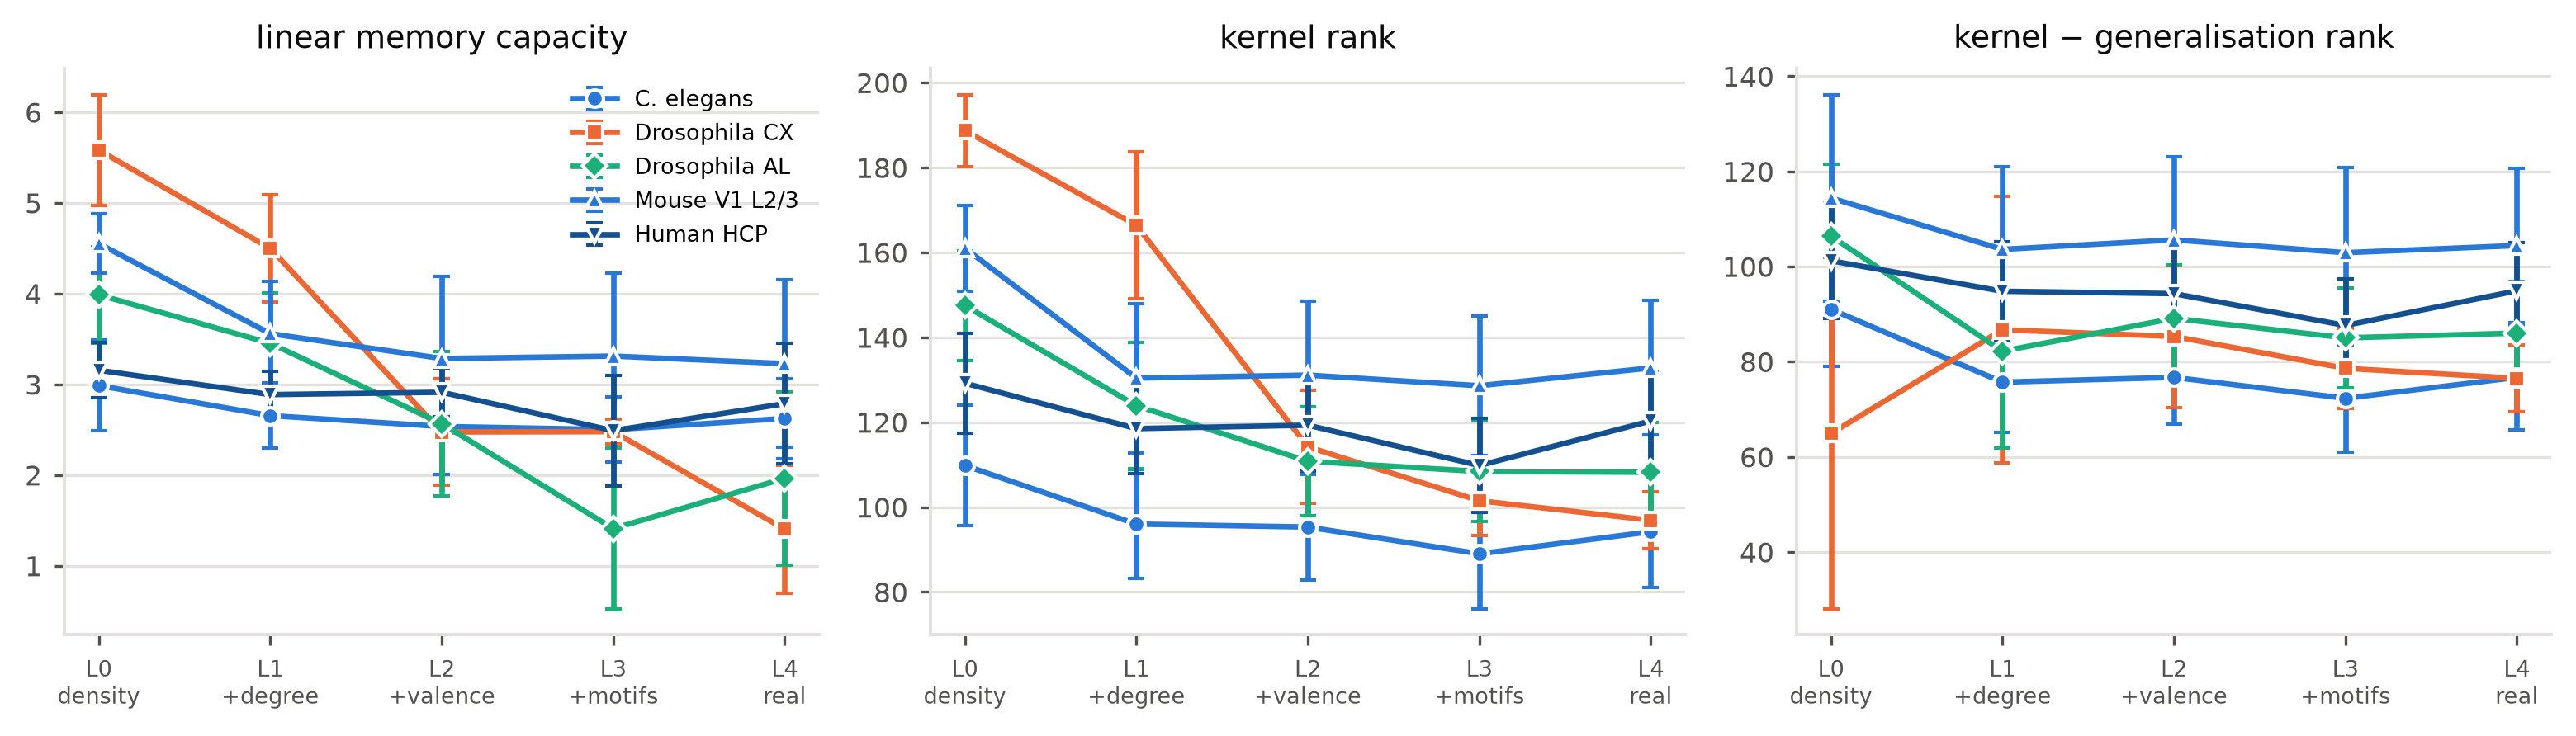
\includegraphics[width=\columnwidth]{figures/fig_dynamics.png}
\caption{\textbf{Dynamical probes across the ladder.} Memory capacity, kernel rank and
the capability index (kernel $-$ generalisation rank) as a function of ladder rung. The
probes are independent of the benchmark, and they reproduce its ordering: the
unstructured rung leads, and the decline is concentrated in the early rungs.}
\label{fig:dynamics}
\end{figure}

The probes reproduce the task result, including the part of it we did not expect
(Figure~\ref{fig:dynamics}). The Erd\H{o}s--R\'enyi rung has the higher memory capacity
in $\NDynMemLzeroHigher$ of $\NDynMemNetworks$ networks, by a median factor of
$\DynMemLzeroOverLfour$, and the higher kernel rank in $\NDynKernLzeroHigher$ of
$\NDynKernNetworks$, by $\DynKernLzeroOverLfour$. So the connectomes are not trading
task accuracy for some capability the benchmark fails to reward; they have less of the
capability the probes measure.

The ordering of properties also carries over. Imposing the degree sequence lowers memory
capacity in $\NDynMemDegreeNeg$ of $\NDynMemNetworks$ networks (median Hedges'
$g = \DynMemDegreeMedG$) and kernel rank in $\NDynKernDegreeNeg$ of
$\NDynKernNetworks$ ($g = \DynKernDegreeMedG$), while the motif census moves them least
of any rung ($g = \DynMemMotifMedG$ and $\DynKernMotifMedG$). After Holm correction
$\NDynMemSig$ of $\NDynMemTotal$ contrasts survive in memory capacity and
$\NDynKernSig$ of $\NDynKernTotal$ in kernel rank --- in both cases the same one, valence
placement in the \textit{Drosophila} central complex, the network whose edges are
two-thirds inhibitory.

The two classes of measurement agree on the direction --- every resolvable effect is
negative, and the unstructured rung leads --- and they agree that the degree sequence
carries the largest share. They do \emph{not} agree on the motif rung. On task accuracy
the motif census produces an effect comparable to the degree sequence's
($\MotifEffectMedian$ against $\DegreeEffectMedian$); on the dynamical probes it is the
smallest contrast in the ladder. We do not have an account of that divergence and do not
want to manufacture one. The most likely reading is that the probes measure properties of
the state ensemble that the ridge readout does not fully exploit, so a structural change
can cost task accuracy without costing measured capacity --- but that is a conjecture, and
the honest summary is that the benchmark and the probes concur on the headline ordering
and part company on one rung of it.

\subsection{Degeneracy is a property of directions}
\label{sec:res-degeneracy}

\begin{figure*}[t]
\centering
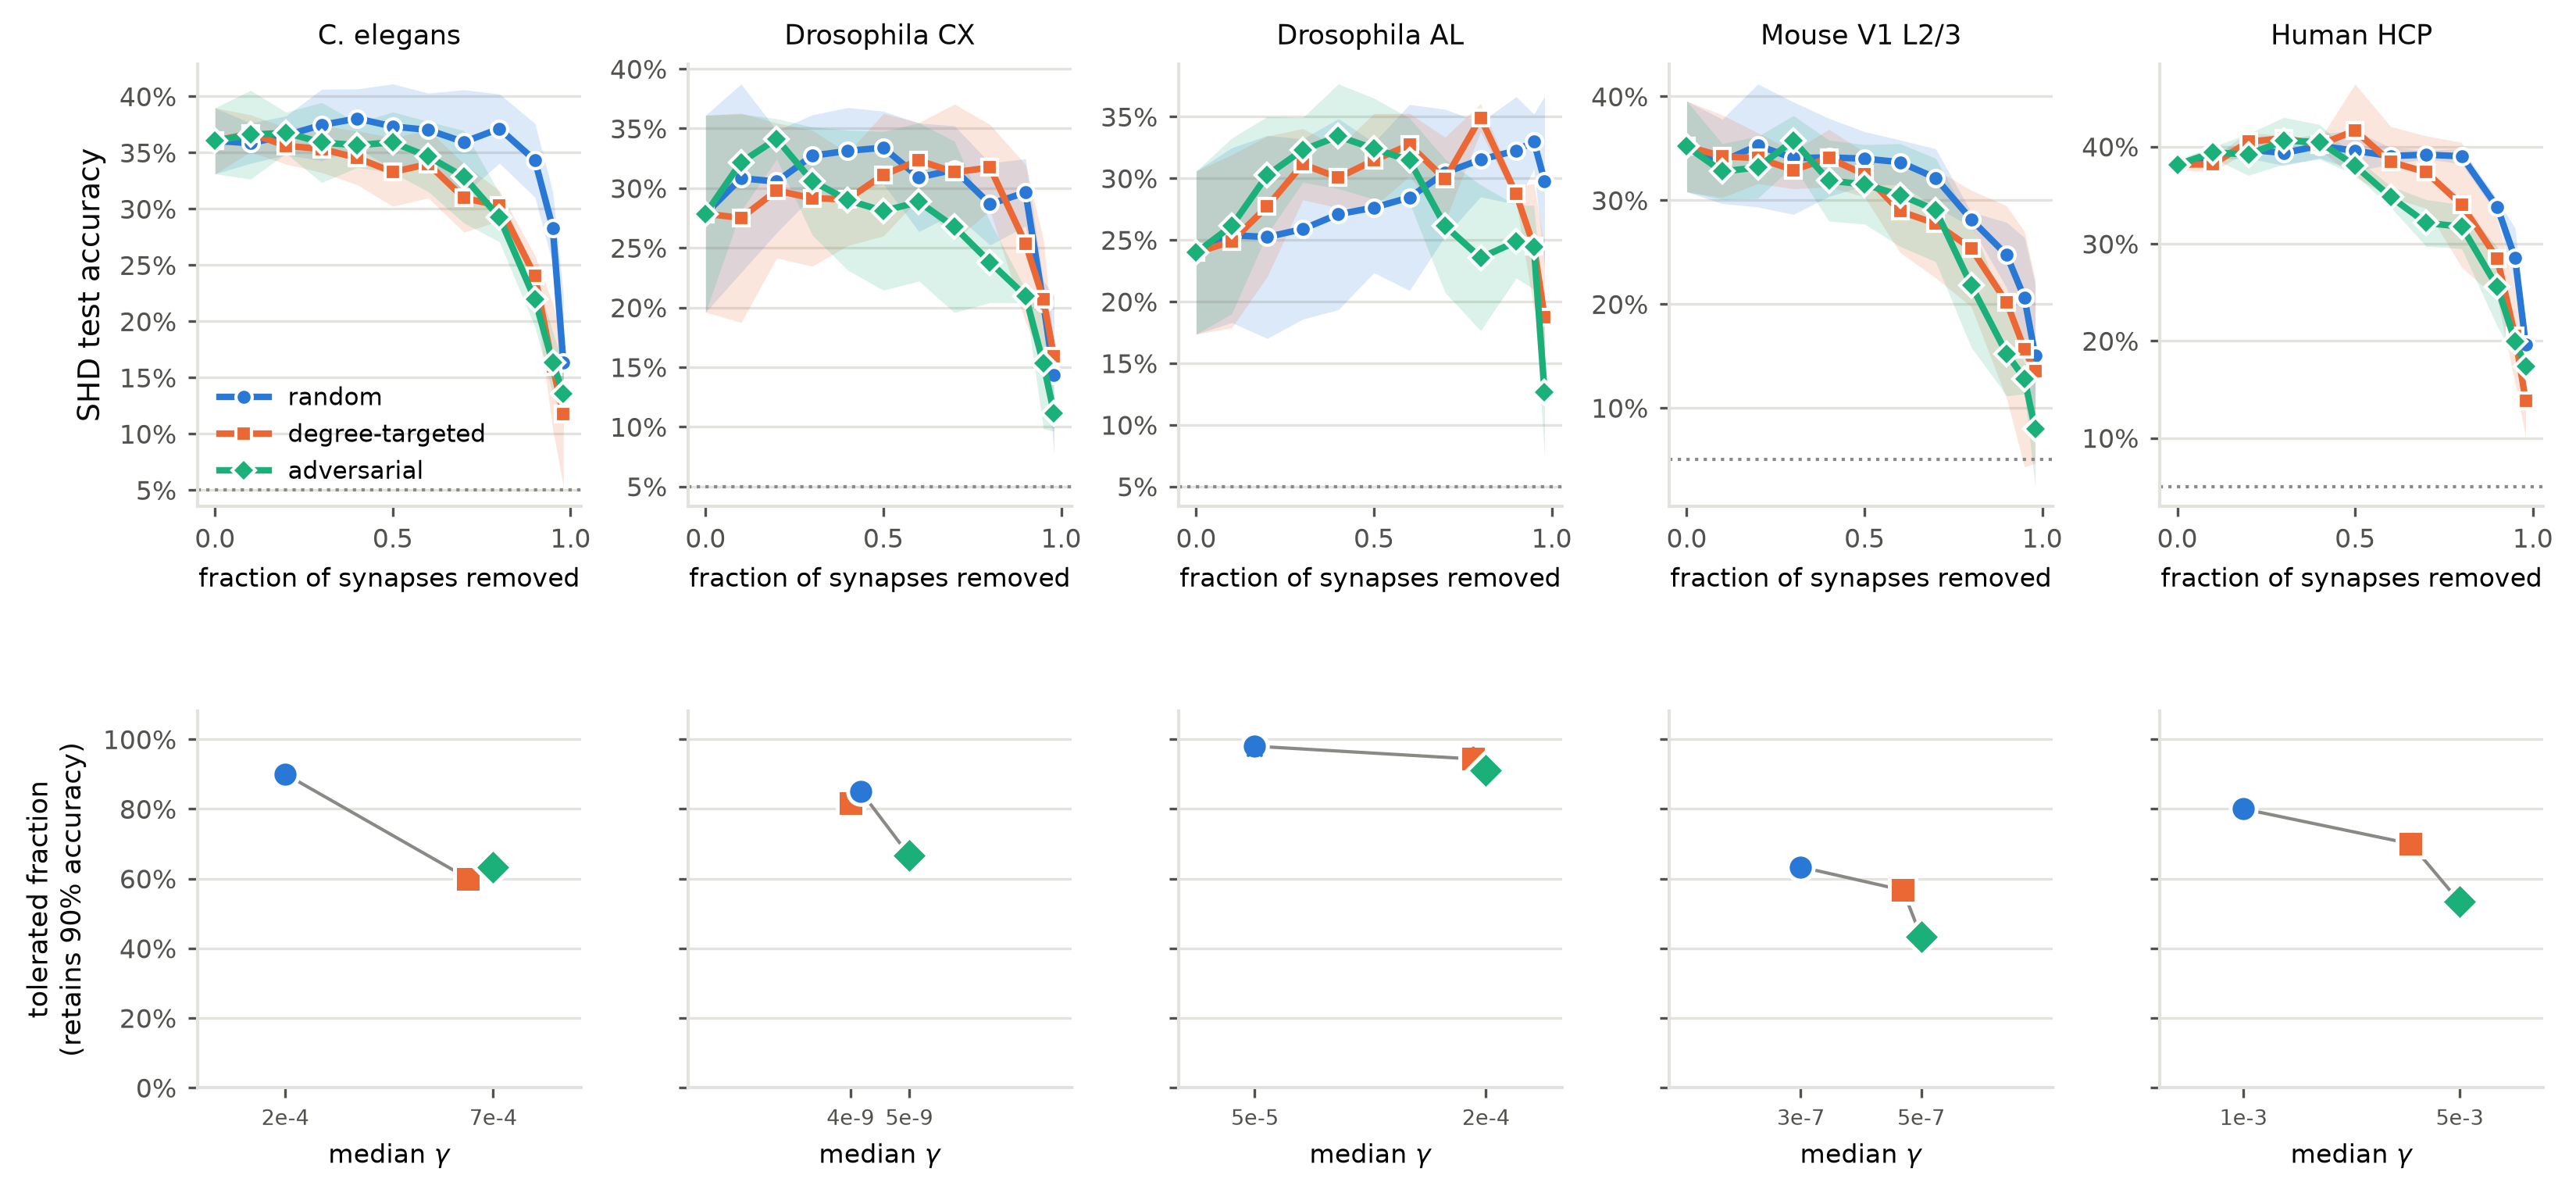
\includegraphics[width=0.95\textwidth]{figures/fig_pruning.png}
\caption{\textbf{Tolerance to synaptic removal depends on direction, not magnitude.}
\textbf{Top:} accuracy against the fraction of synapses removed, for uniformly random
pruning, degree-targeted pruning, and the first-order maximally damaging ranking, all at
matched spectral radius. \textbf{Bottom:} the ordinal prediction, tested within each network --- tolerated
fraction against median $\gamma$, one point per strategy. If tolerance falls with
$\gamma$ the three points descend left to right, which they do in
$\NGammaOrdered$ of $\NGammaNetworks$ networks. Note the $x$ ranges: $\gamma$ differs
between networks by five orders of magnitude, because it is normalised by a
network-specific worst-case constant, so these panels cannot be merged into one and
a pooled $\gamma$ axis would show nothing. Weight-magnitude
pruning is not shown because it is undefined on these graphs: the connectomes are
unweighted, so every edge has the same magnitude and a ``weakest-first'' schedule is an
index ordering in disguise.}
\label{fig:pruning}
\end{figure*}

The measured spectral gaps of these networks are as small as $\MinSpectralGap$, so the
Davis--Kahan bound admits perturbations of norm at most $\MaxDKAdmissible$ --- far below
any perturbation that a single synapse removal produces. The classical bound is not
loose here; it is inapplicable, and the ratio between empirical tolerance and that bound,
which an earlier revision of this work reported as evidence of biological robustness, is
a property of eigenvector conditioning.

Proposition~\ref{prop:tolerance} instead predicts that tolerance scales inversely with
the operational alignment $\gamma$ of the perturbation direction. We tested that in two
forms, and they do not give the same answer.

\paragraph{The ordinal prediction holds, mostly.}
Within each network, $\gamma$ is larger for the structured directions than for the
random one: relative to uniformly random removal, degree-targeted removal realises
$\GammaRelHub\times$ the worst case and the first-order maximally damaging ranking
$\GammaRelAdv\times$. The tolerated fractions run in the opposite order, as predicted ---
$\RNinetyRand$ for random removal, $\RNinetyHub$ for degree-targeted and $\RNinetyAdv$
for adversarial, a factor of $\RNinetyRatio$ between the extremes at identical
cardinality (Figure~\ref{fig:pruning}). Taken network by network, $\gamma$ orders the
three strategies correctly in $\NGammaOrdered$ of $\NGammaNetworks$.

\paragraph{The quantitative prediction does not.}
The proposition says more than an ordering: it says the tolerated magnitude scales as
$1/\gamma$, so the product $\gamma \cdot \|E\|_F^{\max}$ should be constant across
directions within a network. It is not. That product still varies by a median factor of
$\GammaProductSpread$ between strategies --- a reduction on the $\GammaRelAdv\times$
spread in $\gamma$ alone, but not the collapse the proposition predicts. We report this
as a partial failure of our own prediction rather than restricting the claim to the
ordering after the fact: $\gamma$ identifies which direction is more damaging, and does
not correctly predict by how much.

\paragraph{$\gamma$ is not comparable between networks.}
One property of $\gamma$ deserves emphasis because it is easy to misuse, including by
us. It is a realised fraction of a worst-case constant $C(T,a)$ that depends on
$\|A\|_2^{\,T}$, and across our five networks the median $\gamma$ spans a factor of
$\GammaSpanAcrossNetworks$. Absolute $\gamma$ values are therefore meaningful only
within a network, and pooled medians across networks --- which an earlier version of
this analysis reported --- are not a quantity at all. Every comparison above is made
within a network and then aggregated.

\paragraph{An unexpected feature of the survival curves.}
All three strategies \emph{improve} accuracy at low pruning fractions, peaking around
$40$--$60\%$ of synapses removed before declining (Figure~\ref{fig:pruning}). These
reservoirs are over-connected for the task, and the improvement is consistent with the
ladder's main finding: removing synapses attenuates exactly the degree heterogeneity
that the L0\,$\rightarrow$\,L1 contrast shows to be costly here. It also means the
tolerated fraction is a conservative summary, and that several random-pruning runs still
retain 90\% of unpruned accuracy at the largest fraction we tested, so $\RNinetyRand$ is
a lower bound.

This is the substantive point, and it survives the partial failure above. Robustness to
randomly chosen ablation is close to generic for large recurrent systems, because a
random direction is nearly orthogonal to any fixed functional subspace. Reporting it as
evidence of biological degeneracy overstates what has been shown: the same networks are
markedly more fragile to a perturbation of identical cardinality chosen along a damaging
direction. A degeneracy claim is only as strong as the worst direction it has been
tested against, and that conclusion needs only the ordering, which holds.

\subsection{What the accompanying hardware actually costs}
\label{sec:res-hardware}

\begin{table}[t]
\centering\small
\caption{\textbf{Logic synthesis of the accompanying RTL} with Yosys and ABC onto the
Nangate45 Open Cell Library (typical corner). These are the quantities this flow can
establish. No die area, power or energy-per-operation figure is reported: the flow
performs no placement, routing, clock-tree synthesis or parasitic extraction. No clock
frequency is reported either, because the toolchain ships no static timing analyser. The
commercial-process figures reported in earlier revisions of this project were never
measured and are withdrawn.}
\label{tab:synthesis}
\resizebox{\columnwidth}{!}{%
\begin{tabular}{lrrr}
\toprule
\textbf{Module} & \textbf{Cells} & \textbf{Flip-flops} &
\textbf{Cell area ($\mu$m$^2$)} \\
\midrule
\texttt{dendritic\_lif\_core} & 4,401 & 70 & 5,301 \\
\texttt{synaptic\_accumulator} & 19,649 & 8,192 & 63,361 \\
\texttt{aer\_crossbar\_router} & 39 & 17 & 124 \\
\texttt{cen\_accelerator\_top} & 590,116 & 25,644 & 749,263 \\
\bottomrule
\end{tabular}}
\end{table}


Table~\ref{tab:synthesis} reports logic synthesis of the accompanying RTL onto an open
cell library. We report gate count, flip-flop count and mapped pre-layout cell area, and
nothing else: this flow performs no placement, routing or parasitic extraction, so die
area and switching power are not determined by it, and it ships no static timing
analyser, so no clock frequency is claimed either. The commercial-process figures quoted in earlier revisions of this project --- a
28\,nm node, a die area, a picojoule-per-operation efficiency --- were produced by a
Python model with those values written in as constants, not by any synthesis flow, and
are withdrawn.

\section{Discussion}

\subsection{What the ladder does and does not license}

The decomposition reported in \S\ref{sec:res-ladder} is a statement about one class of
models: fixed recurrent reservoirs with a trained linear readout, evaluated on one
spike-based classification task at matched size, density and spectral radius. Within
that class, the attribution is clean, because adjacent rungs differ in exactly one
structural property and nothing else. Outside it, five caveats apply, and only one of them
can be resolved by more instances of the same experiment.

First, the readout is linear and the recurrent weights are untrained. A structural
property might matter for \emph{learnability} -- how readily a network is shaped by a
learning rule -- while being invisible to a fixed-reservoir probe. Motif structure has
been argued to act as an inductive bias, and an inductive bias is by definition a claim
about learning trajectories, not about the function computed by a frozen network. Our
result does not test that claim, and the natural next experiment is to run the same
ladder with the recurrent weights trained by surrogate-gradient descent
\cite{neftci2019surrogate,zenke2021remarkable}, where the rungs would differ in
initialisation rather than in final connectivity. We flag one trap in that experiment,
having walked into it: with only a fraction of neurons driven, a firing-rate penalty
strong enough to be useful in an all-to-all network makes total silence the global
optimum, and a collapsed network returns a perfectly flat ladder that is
indistinguishable from the result reported here. A trained ladder should therefore
report its zero-recurrence control and its mean firing rate before it reports anything
else.

Second, all weights are binary up to valence. Real synapses have graded strengths that
correlate with topological position, and a motif census computed on the binarised graph
discards that correlation. A weighted motif-preserving null is a natural extension; the
annealed chain generalises to weighted targets without modification, but the
degree-preserving move set does not.

Third, the motif-preserving chain is annealed, and annealing is not proven to sample
uniformly over the constraint set. We report mean pairwise overlap between ensemble
members as evidence that the chain explores that set rather than collapsing onto one
region of it (Table~\ref{tab:nullval}), and we show in \S\ref{sec:res-robust} that the
conclusion survives an eightfold variation in chain length and does not depend on which
of the two possible starting points the chain uses. Those checks rule out the two
specific ways an annealed sampler could manufacture a null contrast; they are not a
uniformity guarantee, and a formally exact sampler for a census-constrained
degree-preserving ensemble remains open. We note what would be at stake if the ensemble
were meaningfully non-uniform: the bias would have to correlate with reservoir accuracy
to produce the flat ladder we observe, and the chain's objective makes no reference to
the task, the input projection or the readout.

Fourth, the null contrasts are bounded by power rather than by measurement: at
$\NinstancesLadder$ surrogates per rung the design resolves $d = \MDEHolm$ at the Holm
worst case, so a moderate motif effect would not have been detected. We report the bound
in \S\ref{sec:res-ladder} rather than presenting the null as though it excluded any
effect at all.

Fifth, the benchmark is a 20-class classification with a one-second horizon. Tasks that
demand memory beyond the intrinsic time constants, or that require a specific dynamical
regime, might be more sensitive to recurrent structure. We partly address this with
task-independent dynamical probes (\S\ref{sec:res-dynamics}), which agree with the task
result, but agreement across two measures is not agreement across all of them.

A further objection applies specifically to the degree-sequence result, and we checked
it rather than argued it. Three of the five networks are induced subgraphs grown by
breadth-first expansion from an above-median-degree seed, and growing outward from a hub
is exactly the sampling that could concentrate high-degree nodes and so inflate the
property the effect is attributed to. Measured as the coefficient of variation of total
degree, extraction does not concentrate it: the ratio of subgraph to full-release
heterogeneity is at most $\MaxCVRatio$ across all five networks, and as low as
$\MinCVRatio$ among the $\NExtractedNetworks$ that are genuinely subsampled, with the
remaining $\NWholeNetworks$ used whole. If the extraction biases the degree result at
all, it does so against it.

\subsection{What a unit model decides}

The result of \S\ref{sec:res-unit} is the one we would most like to be wrong about, so we
have tried to state it at exactly its strength and no further.

What it establishes is narrower than the draft of this section that preceded
\S\ref{sec:res-nullchoice}, and we have rewritten it rather than leaving the stronger
phrasing standing. That draft said an advantage unambiguous in graded units was absent in
spiking ones. Against the published null there is no unambiguous advantage in graded units
to be absent: what remains is that the two model classes do not give the same answer on
identical graphs, and that capacity in the spiking model is compressed by a factor of
$\UnitCapRatio$, so effects of the reported size sit near the resolution of the
measurement there. It does not establish that connectome topology is useless in spiking
systems --- one network in our set is at the capacity floor and carries no information
either way --- nor that memory capacity is the right currency.

The mechanism is the one claim in this paper that the null correction moved in our favour,
and it is worth saying so explicitly because we had already published the opposite.
Measured against the ensemble we first built, differential silencing did not predict the
capacity gap and we wrote it up as a failed prediction. Measured against the published
ensemble it does ($r = \UnitSilenceGapR$, $p = \UnitSilenceGapP$, $n =
\UnitSilenceGapN$). We hold the surviving version to the same standard as the discarded
one: it accounts for part of the spiking arm's behaviour in the predicted direction and
leaves most of the variance unexplained.

What we think it does establish is a constraint on how the result should be used. The
connectome-reservoir finding is cited as evidence that biological wiring is computationally
special, and that inference is doing work in proposals for neuromorphic hardware built on
connectome-derived connectivity. Neuromorphic hardware is spiking. Whatever the advantage
measured in $\tanh$ units is worth, the inference from it to a spiking substrate needs its
own evidence --- and on our measurements that evidence does not exist in either direction
yet, because the comparison is weaker in the spiking model rather than resolved there.

We would put the general form of this more plainly than the specific result. A reservoir
result is a statement about a triple: a graph, a unit model and an operating point. Two of
those three are usually chosen once and reported as fixed --- and the null, a fourth, is
usually named rather than specified. We varied all four and the conclusion turns on each.
The methodological recommendation is unglamorous and cheap: report the unit model as a
variable rather than an implementation detail, sweep the gain rather than picking a point
on it, and ship the null-generating code.

\subsection{What the gain axis does to a literature}

The result of \S\ref{sec:res-operating} is uncomfortable in a specific way, and we want to
state the discomfort precisely rather than soften it.

It is not that the published connectome advantage is wrong. It is that the quantity being
reported is a point on a curve whose sign changes, and the curve has not been shown. Our
own attempt to recover the published direction at the published operating point succeeds
against one null ensemble and fails against the other (\S\ref{sec:res-nullchoice}), which
is a reason to doubt our replication rather than the original --- and which makes the
point of this section sharper, not weaker: a single evaluation carries no information
about where on the curve, or against which ensemble, it was taken. Nothing in a
single-operating-point comparison indicates which side of the crossing it falls on, and
nothing in the reported statistics --- ours or anyone's --- carries that information,
because the statistics are computed conditional on the choice.

We think the reason this has gone unremarked is that criticality is a principled choice.
There are good arguments that a reservoir computes best near the edge of chaos
\cite{bertschinger2004real,legenstein2007edge,boedecker2012information}, and if biological
networks operate there, comparing at criticality is comparing where it matters. The
difficulty is that the argument licenses the operating point but not the inference: a
topology can be better at criticality and worse elsewhere without either fact being the
more fundamental one, and ``connectome topology confers computational function'' is a
claim of the second kind stated on evidence of the first.

There is also an asymmetry in the direction of the effect that we think is the more
interesting result. The published comparison is against a \emph{degree-preserving} null.
Against a fully unstructured graph of the same size and density, the connectome does not
lead at any gain we tested. So the advantage that appears at criticality is an advantage
over graphs that share the connectome's degree sequence --- and the degree sequence is,
by our ladder, the single most costly structural property on this task. The narrow win
at criticality sits on top of a large loss that the degree-preserving control holds
constant and therefore hides.

What we would ask of a future comparison of this kind is small: report the contrast across
a range of gains, and state the range over which the sign is stable. That is one sweep
rather than one evaluation, and it converts a claim about a point into a claim about a
regime. We have tried to hold our own results to it.

\subsection{Why matched controls change the conclusion}

The reason a control ladder matters here is arithmetic rather than philosophical. An
Erd\H{o}s--R\'enyi comparison bundles every structural difference into a single contrast,
so whatever it finds gets attributed to whichever property the authors were already
interested in. In our measurements that bundled effect is not small --- the
Erd\H{o}s--R\'enyi rung leads the connectome by up to $\RmLzeroMinusLfour$ of accuracy
in percentage points at
a matched operating point --- which makes the attribution question sharper rather than
moot. Separating the properties shows that the largest single share is spent at the step that
imposes the degree sequence, and that the motif census contributes a further effect of
comparable size --- in the same, negative direction. An Erd\H{o}s--R\'enyi comparison on
this benchmark delivers a large, significant, correctly-signed aggregate effect that a
motif-focused reading would have assigned to motifs. Part of it is indeed the motif
census; most of it is not, and none of it points the way that reading would require. That
is the concrete cost of the bundled control, and it is why we regard the ladder as the
contribution here rather than the result it produces.

This is also where the protocol control in \S\ref{sec:task} does the most work. A
reservoir comparison in which a zeroed recurrent matrix performs as well as a connectome
is not a weak experiment; it is a measurement of the input projection. We report both
protocols precisely because the difference between them dwarfs every structural effect we
measure, and because the failure is silent: nothing in the naive protocol's output
announces that recurrence is unused. We would encourage the same control in any
study comparing connectome-derived reservoirs.

\subsection{Degeneracy is a statement about directions, not magnitudes}

The pruning results in \S\ref{sec:res-degeneracy} make a point that we think is
under-appreciated. Robustness to random ablation is routinely reported as evidence that
biological circuits are degenerate, redundant or gracefully degrading. But a randomly
chosen perturbation direction in a high-dimensional space is nearly orthogonal to any
fixed functional subspace, so tolerance to random damage is close to a generic property
of large recurrent systems rather than a distinguishing property of brains. The
operational alignment $\gamma$ makes part of this quantitative: the same perturbation
cardinality can be almost harmless or markedly damaging depending only on its direction,
and $\gamma$ ranks the directions correctly. It does not deliver the scaling
Proposition~\ref{prop:tolerance} predicts --- the product $\gamma\cdot\|E\|_F^{\max}$
should be constant across directions and instead varies by a factor of
$\GammaProductSpread$ (\S\ref{sec:res-degeneracy}) --- so $\gamma$ should be read as a
diagnostic of which directions are dangerous rather than as a calibrated predictor of how
much damage they do. A degeneracy claim is nonetheless only as strong as the worst
direction it has been tested against, and that conclusion needs only the ordering.

We also note what replacing Davis--Kahan buys. The eigenvector bound is not merely loose
on these networks; it is inapplicable, because the spectra are near-degenerate and the
eigenvectors it bounds are themselves ill-conditioned. Quoting the ratio between an
empirical tolerance and a vacuous bound as a measure of biological robustness -- as an
earlier revision of this work did -- attributes to the system a property of the tool.
The transfer-map bound is weaker in the usual sense (it is first-order and
horizon-limited) but it is about a quantity that task performance actually depends on,
and it requires no gap.

\subsection{A method sentence is not a method}
\label{sec:disc-null}

The single most consequential finding in this paper is also the least glamorous: the
phrase ``randomised while preserving density and degree sequence'', which appears in some
form in nearly every paper in this literature, does not specify an ensemble. Two
constructions satisfying it gave the connectome's advantage opposite significant verdicts
in $\NNullVerdictFlip$ of $\NNullCells$ cells (\S\ref{sec:res-nullchoice}). The ambiguity
is not exotic. It is whether a weight is a property of an edge or a property of the
network's weight distribution, and both readings are natural enough that the phrase has
carried them both for two decades.

We are the demonstration and not the auditor here. Our first implementation was the
rank-reassigning one, written from the published description without reading the toolbox
source, and it produced a result that was clean, large, significant in every network and
in the direction we expected. Nothing about it looked wrong, because nothing about it was
wrong except the question it was answering. Had the two ensembles happened to agree, we
would have reported the number and moved on, and the paper would have contained an
undetectable error of exactly the kind we spent the rest of it cataloguing.

Two consequences follow, and neither is a matter of care. The first is that a replication
which constructs its null from a published description is testing a different hypothesis
from the original, and cannot tell which of the two it has tested. The second is that the
remedy is not more careful prose --- we do not think a longer sentence would have saved
us --- but the null-generating code as an artefact, cited and versioned the way a dataset
is. Where the original code exists, as it does here, calling it is not a courtesy to the
original authors; it is the only way to know what was compared.

This generalises past reservoir computing. Motif enrichment, small-worldness, rich-club
coefficients and every other statistic in network neuroscience defined as a deviation from
a null inherit whatever ambiguity the null's description carries. The $Z$-scores we report
in \S\ref{sec:res-motifs} are no exception, and we state the construction we used in the
methods for that reason.

\subsection{On correcting the record}

A substantial part of this work consisted of removing claims from our own earlier
manuscript: fabricated commercial-process silicon figures, a human microscale tier built
on a connectivity graph that was empty, sign-attributed motif results for datasets with
no usable inhibition, p-values below the resolution of the null ensemble that produced
them, and an ablation table whose own control row contradicted the conclusion drawn from
it. We report these in full in the accompanying audit rather than quietly omitting them,
because the corrected analysis is only interpretable against the record of what it
replaces, and because several of the errors are of kinds that are easy to reproduce:
a silently swallowed exception in a loader, a null model believed to impose a constraint
that it does not, and a benchmark protocol under which the object of study makes no
difference to the result.

The replacement analysis produced four more of the same kind, and we record those too.
The largest is the null-ensemble substitution discussed above, which is not a coding
error at all --- the code did exactly what it was written to do --- but a
misreading of a method sentence that no test could have caught.
Our annealing energy was normalised by a quantity several times larger than the one the
methods described, which left the chain unable to hold its census on the most reciprocal
network in the set. Our ``weakest-first'' pruning arm was executing as whole-neuron
ablation in index order, because these graphs are unweighted and every edge magnitude is
therefore equal. And the first version of Proposition~\ref{prop:gapfree} was stated in
the spectral radius rather than the operator norm, an inequality that holds only for
normal matrices --- in a paper whose central argument is that eigenvalue-based reasoning
fails on these networks. Each was caught by checking a diagnostic that the code already
recorded, or by checking the code against the prose; none was caught by the result
looking wrong, because in every case it did not. We take that to be the substantive
methodological point, and it is why the convergence diagnostics, the protocol control
and the held-out statistic are reported in the paper rather than kept in the
repository.

\subsection{Coupling is a relation, not a property}
\label{sec:disc-coupling}

It is worth stating plainly what the four results have in common, because it is the
thing the title names. Computational coupling --- the degree to which what a network
computes is attributable to how it is wired --- reads like a property of the network, and
is written down that way: one connectome, one number, one verdict. Definition~\ref{def:coupling}
makes explicit that it is nothing of the kind. $\kappa$ takes four arguments besides $W$,
and this paper is an empirical demonstration that none of them is inert. Change
$\mathcal{N}$ and the sign flips in $\NNullVerdictFlip$ of $\NNullCells$ cells with
significance on both sides. Change $U$ and the whole capacity scale compresses by
$\UnitCapRatio\times$, taking the contrast with it. Move along $\rho$ and the sign flips
again, in $\NGainSignFlip$ of $\NGainNetworks$ networks. Choose $R$ badly and the coupling
is identically zero: deleting the recurrent matrix costs nothing
($\ZeroRecFull$ against $\ZeroRecFullConn$), which is to say the measurement was never
touching $W$.

The practical consequence is a reporting standard rather than a new experiment. A
coupling is quotable only with its protocol attached --- and, given
\S\ref{sec:res-nullchoice}, with the null-generating code attached rather than a
description of it, since the description does not determine the ensemble. Where a claim
is meant to be about the connectome rather than about one cell of the design, the
defensible object is not a number but a surface: $\kappa$ over the ranges of
$\mathcal{N}$, $U$, $\rho$ and $R$ that the claim is supposed to survive. That is
why we report axes rather than points throughout, including for our own null results,
and it is why a non-detection here is reported as a non-detection rather than as a
refutation.

We do not claim the four are exhaustive. They are the four our design happened to vary,
and the honest reading of Definition~\ref{def:coupling} is that any further argument
smuggled into $C$ --- the task, the horizon, the delay structure, the regularisation of
the readout --- is a further candidate for the same treatment. The claim we do make is
narrower and, we think, secure: a connectome-versus-null result reported as a single
signed number is under-determined by its own methods section, and on our data the
under-determination is large enough to reverse the conclusion.

\subsection{Outlook}

The motif-preserving ensemble is not specific to neuroscience. Any field that infers
function from subgraph overrepresentation -- gene regulatory networks, food webs,
software dependency graphs -- faces the same attribution problem, and the same annealed
construction applies wherever a motif census admits incremental evaluation. The
immediate extensions we regard as most informative are the trained ladder described above,
applying $\gamma$ to measured biological perturbations --- where the prediction is that
developmental and activity-dependent rewiring occupies the low-$\gamma$ regime that makes
degeneracy cheap --- and extending the null-sensitivity analysis of
\S\ref{sec:res-nullchoice} beyond the two constructions we happened to write. We suspect
the two we compared are not the only pair in circulation under that description, and the
cheapest useful contribution anyone could make to this literature is an inventory of
which published results were measured against which ensemble.


\section*{Data and code availability}
All connectome data used here are public releases, cited at first use. The Spiking
Heidelberg Digits dataset is distributed by the Zenke laboratory. Analysis code,
null-model implementations, experiment drivers and the synthesis flow are in the
accompanying repository; every figure and table in this paper is regenerated from
raw result files by \texttt{src/analysis/rebuild\_paper.sh}, and every number in the
text is drawn from a machine-generated macro file rather than transcribed by hand ---
a missing result appears in the compiled PDF as a visible placeholder rather than as a
stale value, and the build reports unresolved placeholders, undefined references and
\LaTeX{} errors rather than relying on the build exiting cleanly.

The repository also carries \texttt{AUDIT.md}, which records every claim withdrawn from
the previous version of this project and the evidence against it, together with the
defects found in the replacement analysis while preparing this one. The retracted
manuscript, its figures, its result files and the executive pitch dossier built on them
are kept under \texttt{paper/superseded\_v4/} and \texttt{results/superseded\_v4/},
labelled as withdrawn, so that the retraction can be checked against what was actually
claimed.

\section*{Author contributions}
A.R.P. designed the study, implemented the methods, ran the experiments and wrote the
manuscript. S.G. contributed to the null-ensemble and ladder experiments, the audit of
the withdrawn claims, and the revision of the manuscript. The work was carried out under
the guidance of J.J.P., who supervised the project and revised the manuscript.

\section*{Competing interests}
The authors declare no competing interests.

\bibliographystyle{unsrt}
\bibliography{../sources/bib/sources}

\end{document}
